\PassOptionsToPackage{quiet}{fontspec}
\documentclass[oneside]{ctexbook}
\usepackage{amsthm,amssymb,amsmath}
\usepackage{fancyhdr}
\usepackage{enumerate}
%\usepackage{biblatex}
\usepackage{biblatex}
\usepackage{graphicx}
\usepackage{picinpar}
\usepackage{subfig}
%\usepackage{epstopdf}
\usepackage{epsfig}
\usepackage{etoolbox}
\usepackage{showidx}
\usepackage{imakeidx}
\usepackage[colorlinks=true]{hyperref}
%\usepackage[yyyymmdd,hhmmss]{datetime}
\setlength{\headheight}{13pt}
\pagestyle{fancy}
%\rfoot{编译时间:  \today\  \currenttime}
%\cfoot{}
%\lfoot{页码:\thepage}
\newcommand{\norm}[1]{{\left | \left |  #1  \right | \right |}}
\newcommand{\inner}[2]{{\left < #1, #2 \right >}}
\newcommand{\abs}[1]{{\left | #1 \right |}}
\newcommand{\parallelsum}{{\mathbin{\!/\mkern-5mu/\!}}} %斜的平行线
\newcommand{\Hn}{{\mathbb{H}^n}}
\newcommand{\Sn}{{\mathbb{S}^n}}
\newcommand{\En}[1]{{\mathbb{R}^{#1}}}
\newcommand{\area}[1]{{\mathcal{A}({#1})}}
\newcommand{\areap}{{\mathcal{A}_{+}}}
\newcommand{\arean}{{\mathcal{A}_{-}}}
\renewcommand{\div}{{\text{div}}}
\newcommand{\spt}{{\text{spt}}}
\newcommand{\tr}{{\text{tr}}}
\newcommand{\sing}{\mathcal{S}}
\newcommand{\proj}{\text{Proj}}
\newcommand{\diam}{\text{diam}}
\newcommand{\Tr}{\text{Tr}}
\newcommand{\XX}{{\vec{X}}}
\newcommand{\cl}[1]{\overline{#1}}
\newcommand{\eq}{\equiv}
%\newcommand{\C}{\mathbb{C}}
\newcommand{\R}{\mathbb{R}}
\newcommand{\nullset}{\emptyset}
\renewcommand{\H}{\mathbb{H}}
\newcommand{\N}{\mathbb{N}}
%\newcommand{\G}{\mathcal{G}}
\renewcommand{\abs}[1]{\left | #1 \right |}
\newcommand{\subsub}{{\subset \subset}}
\newcommand{\OR}{{\Omega \times \mathbb{R}}}
\newcommand{\OL}{{\Omega_L}}
\renewcommand{\epsilon}{\varepsilon}
\renewcommand{\phi}{\varphi}

\renewcommand{\l}{{\lambda}}
%\renewcommand{\L}{{\Lambda}}
\newcommand{\e}{{\epsilon}}
\newcommand{\E}{{\Epsilon}}
\renewcommand{\d}{{\delta}}
\newcommand{\D}{{\Delta}}
\newcommand{\g}{{\gamma}}
\newcommand{\G}{{\Gamma}}
\renewcommand{\a}{{\alpha}}
\newcommand{\A}{{\Alpha}}
\renewcommand{\b}{{\beta}}
\newcommand{\B}{{\Beta}}
\renewcommand{\u}{{\mu}}
%\newcommand{\U}{{\Mu}}
\renewcommand{\v}{{\nu}}
\newcommand{\V}{{\Vu}}
\newcommand{\x}{{\times}}
\newcommand{\s}{{\quad}}
\renewcommand{\ss}{{\qquad}}
\newcommand{\sss}{{\qqquad}}
\renewcommand{\L}{\mathcal{L}}
\renewcommand{\D}{{D}}
\newcommand{\aij}{{a^{ij}}}
\newcommand{\dij}{{D_{ij}}}
\newcommand{\tto}[1]{{{\xrightarrow{#1}}}}
\renewcommand{\P}{{\partial}}
\newcommand{\PT}{{\partial_t}}
\newcommand{\PTF}{{\partial_t F}}
\newcommand{\PI}{{\partial_i}}
\newcommand{\PJ}{{\partial_j}}
\newcommand{\PIF}{{\partial_i F}}
\newcommand{\PJF}{{\partial_j F}}
\newcommand{\vt}{{d\mu_t}}
\newcommand{\vv}{{d\mu}}

\newcommand{\GG}{{\mathfrak{G}}}
\newcommand{\BR}{{B_r(x)}}
\newcommand{\GR}{{\GG \times \mathbb{R}}}
\newcommand{\EG}{{\mathfrak{E}}}
\newcommand{\HH}{{\tilde{H}}}
\newcommand{\BVG}{{BV(\GG,\psi)}}
\newcommand{\BVO}{{BV(\Omega)}}
\newcommand{\PO}{{\partial \Omega}}
\newcommand{\overl}[1]{{\overline{#1}}}
\newcommand{\ol}[1]{{\overline{#1}}}
\newcommand{\oo}{{\infty}}
\renewcommand{\O}{\Omega}
\newcommand{\Poincare}{\text{Poincar\'e}}
\newcommand{\Holder}{\text{{H\"older}}}
\newcommand{\reciprocal}[1]{{\frac{1}{#1}}}
\newcommand{\rec}[1]{{\reciprocal{#1}}}
\renewcommand{\e}{\text{e}}
\newcommand{\iin}{\text{ in }}
\newcommand{\supp}{\text{supp}}
\newcommand{\osc}{\mathop{\text{osc}}}
\newcommand{\loc}{\text{loc}}
\newcommand{\SSP}[1]{{\S^+(\lambda,\Lambda,#1)}}
\newcommand{\SSN}[1]{{\S^-(\lambda,\Lambda,#1)}}
\renewcommand{\SS}[1]{{\S(\lambda,\Lambda,#1)}}
\renewcommand{\S}{\mathbb{S}}
\renewcommand{\N}{{N}}
\newcommand{\Hull}{{\text{Conv}}}
\newcommand{\MN}[1]{{\mathcal{M}^-(\lambda,\Lambda,#1)}}
\newcommand{\MP}[1]{{\mathcal{M}^+(\lambda,\Lambda,#1)}}
%\renewcommand{\iff}{\Leftrightarrow}
\renewcommand{\iff}{\Longleftrightarrow}
\newcommand{\semiholder}[1]{{[#1]}}
\newcommand{\lsc}[1]{{\text{LSC}(#1)}}
\newcommand{\usc}[1]{{\text{USC}(#1)}}
\renewcommand{\G}{\text{Graph}}
\newcommand{\CC}{{C^\infty_0}}
\newcommand{\ddt}{\frac{d}{dt}}
\newcommand{\ddtt}{\frac{d^2}{dt^2}}
\newcommand{\ddr}{\frac{d}{dr}}
\newcommand{\ppt}{\frac{\partial}{\partial_t}}
\newcommand{\Area}{\text{Area}}
\newcommand{\MM}{{\tilde{\mathcal{M}}}}
\newcommand{\M}{{\mathcal{M}}}
\newcommand{\tangent}{{\text{T}}}
\newcommand{\Laplace}{{\Delta}}
\newcommand{\T}{{\perp}}
\newcommand{\DD}{{\tilde{\nabla}}}
\renewcommand{\D}{{\nabla}}
\newcommand{\barpartial}{{\bar{\partial}}}
\newcommand{\Haus}{{\mathcal{H}}}
\newcommand{\Res}{{\text{Res}}}
\renewcommand{\Re}{{\mathfrak{Re}}}
\renewcommand{\Im}{{\mathfrak{Im}}}
\newcommand{\II}{{\Pi}}
\newcommand{\HLaplace}{{\Delta}}
\newcommand{\CLaplace}{{\underline{\Delta}}}
\newcommand{\TS}{{\tilde{\Sigma}}}
\newcommand{\CV}{{C^\infty_0}}
\renewcommand{\CC}{{C^\infty_c}}
\newcommand{\NT}{{\nabla}}



\newtheorem{theorem}{定理}[chapter]
\newtheorem{assumptions}{假设}
\newtheorem{lemma}[theorem]{引理}
\newtheorem{proposition}[theorem]{命题}
\newtheorem{exercise}[theorem]{习题}
\newtheorem{corollary}[theorem]{推论}
\newtheorem{definition}[theorem]{定义}
\newtheorem{question}[theorem]{问题}
\newtheorem*{question*}{问题}
\newtheorem{example}[theorem]{例}
\newtheorem*{example*}{例}
\newtheorem*{proposition*}{命题}
\theoremstyle{plain}
\newtheorem{remark}[theorem]{注}
%\newtheorem{claim}[theorem]{断言}
\newtheorem*{claim*}{断言}

\newenvironment{subproof}[1][\proofname]{%
  \renewcommand{\qedsymbol}{$\diamond$}%
  \begin{proof}[#1]%
}{%
  \end{proof}%
}



\usepackage{enumitem,xparse}
\newlist{Claim}{description}{2}
\setlist[Claim]{labelindent=2em,leftmargin=*}
\newif\ifInsideClaim
\newcounter{claim}[theorem]
\newcounter{cclaim}[claim]
\renewcommand\theclaim{\arabic{claim}}
\renewcommand\thecclaim{\arabic{claim}.\arabic{cclaim}}
\let\originalqedsymbol\qedsymbol
\newenvironment{claim}{%
	% disable qed symbol if there is no star
	%\let\qedsymbol\relax%
	%\let\qedsymbol$\diamond$
	\ifInsideClaim% we have a nested environment
	\refstepcounter{cclaim}%
	\let\theclaimcounter\thecclaim%
	\else%
	\refstepcounter{claim}%
	\let\theclaimcounter\theclaim%
	\InsideClaimtrue%
	\fi%
	\Claim\item[\textbf{断言 \theclaimcounter:}]%
}{\endClaim\InsideClaimfalse\let\qedsymbol\originalqedsymbol}



\DeclareSourcemap{
  \maps[datatype=bibtex]{
    \map{
       \step[fieldset=URL, null]
       \step[fieldset=DOI, null]
       \step[fieldset=MRREVIERER, null]
       \step[fieldset=ISBN, null]
       \step[fieldset=ISSN, null]
       \step[fieldset=SERIES, null]
    }
  }
}

%\renewcommand\appendix{\par
%    \setcounter{section}{0}
%    \setcounter{subsection}{0}
%    \gdef\thesection{附录 \Alph{section}}}
%
\addbibresource{minisurf.bib}

\newif\ifshow
%\showtrue % comment out to hide answers

\newif\ifsee
\seetrue

%\def \noperron {}

%\defbibheading{bibliography}[参考文献]{\chapter*{#1}}
\begin{document}
\title{课程:极小曲面}
%\author{主讲:高强}
\author{draft version}
\date{修改日期: {\today}}
%\date{2022年秋季学期}
\maketitle
\tableofcontents
\input{Chapter01}
\chapter{曲率估计}
\section{逐点估计}
设$\Sigma^{n-1} \subset \M^n$是光滑子流形. $\vec{n}$是 $\Sigma$的单位法向. 设$T$是$(0,2)$型张量, $T=T_{ij}dx^idx^j$. 记号约定如下.
\begin{equation}
    (\nabla^2_{XY}T)(Z,W)=\nabla^2T(Z,W,Y,X).
\end{equation}
在局部坐标下,
\begin{equation}
    \nabla^2_{lk}T_{ij}=(\nabla^2_{\partial l,\partial k}T)(\PI,\PJ)=\nabla^2T(\PI,\PJ, \partial k,\partial l)=T_{ijkl}.
\end{equation}
Codazzi方程.
\begin{equation}
    R^\M(X,Y,W,\vec{n}) = \nabla \II(W,Y,X) - \nabla \II (W,X,Y).
\end{equation}
Gauss方程
\begin{equation}
    R^\M(X,Y,Z,W) = R^\Sigma(X,Y,Z,W)-\II(X,W)\II(Y,Z)+\II(X,Z)\II(Y,W).
\end{equation}
求导交换次序.
\begin{equation}
    \nabla^2_{X,Y}T(Z,W) = \nabla^2_{Y,X}T(Z,W)-T(R(X,Y)Z,W)-T(Z,R(X,Y)W).
\end{equation}
在局部坐标下,
\begin{equation}
    T_{ijkl}=T_{ijlk}-R_{lki}^pT_{pj}-R_{lkj}^pT_{ip}.
\end{equation}
求导交换次序的结果可以参考\cite[定理7.14]{lee}. 需要注意, $T_{ijkl}=(\nabla^2_{lk}T)(\PI,\PJ)$.  
\begin{proposition}
    设$\Sigma^{n-1} \subset \R^n$是光滑曲面. $\nabla, \Delta$为$\Sigma$上的算子. $\II$为其第二基本型, $H$是平均曲率. 则
    \begin{equation} \label{simon1}
        \Delta \II_{ij}=\nabla^2_{ij}H + Hg^{kl}\II_{ik}\II_{jl}-\abs{\II}^2\II_{ij}.
    \end{equation}
\end{proposition}
\begin{proof}
    固定点$p$, 选取$p$点附近的测地坐标, 则有
    \begin{equation}
        \Delta \II_{ij}=\II_{ij;kk}=\II_{ik;jk}=\II_{ik;kj}-R_{kji}^p\II_{pk}-R_{kjk}^p\II_{ip}.
    \end{equation}
    而
    \begin{equation}
        \II_{ik;kj}=\II_{kk;ij}=H_{ij}.
    \end{equation}
    \begin{equation}
        \begin{split}
            R_{kji}^p\II_{pk}+R_{kjk}^p\II_{ip} &= R_{kjip}\II_{pk}+R_{kjkp}\II_{ip}\\
            &=\II_{kp}\II_{ji}\II_{kp}-\II_{ki}\II_{jp}\II_{pk}+\II_{kp}\II_{jk}\II_{ip}-\II_{kk}\II_{jp}\II_{ip} \\
            &=\abs{\II}^2\II_{ij}-Hg^{pq}\II_{jp}\II_{iq}
        \end{split}
    \end{equation}
\end{proof}
\begin{proposition}[Simons等式] \label{simon_equation}
    设$\Sigma^{n-1}$是极小曲面, 则有
    \begin{equation}
        \Delta\abs{\II}^2 = 2(\abs{\nabla \II}^2-\abs{\II}^4).
    \end{equation}
\end{proposition}
\begin{proof}
    将等式\eqref{simon1}写成坐标无关的形式, 又因$\Sigma$是极小曲面, 则有
    \begin{equation}
        \Delta \II = -\abs{\II}^2 \II
    \end{equation}
    由于$\Tr$与联络导数可交换, 则
    \begin{equation}
        \begin{split}
            \Delta \abs{\II}^2 = \Delta (\Tr^2(\II\otimes\II)) &= \Tr^2(\Delta \II \otimes\II + \II \otimes \Delta \II + 2 \Tr(\nabla \II, \nabla \II)) \\
            &=\Tr^2(-2\abs{\II}^2 \II\otimes\II+2\Tr(\nabla \II \otimes \nabla \II)) \\
            &=-2\abs{\II}^4+2\abs{\nabla \II}^2.
        \end{split}
    \end{equation}
\end{proof}
\begin{proposition}[Simons不等式]
    设$\Sigma^{n-1}$是极小曲面, $\nabla,\Delta$为$\Sigma$上的算子. 则
    \begin{equation} \label{simon_inequality}
        \Delta \abs{\II}^2 \ge -2\abs{\II}^4+2(1+\frac{2}{n-1})\abs{\nabla \abs{\II}}^2.
    \end{equation}
\end{proposition}
\begin{proof}
    证明与命题\eqref{kato}类似. 我们首先来计算 $\abs{\nabla \abs{\II}}^2$. 固定点$p$, 取$p$点处的测地坐标使得$\II=diag(\lambda_i)$.
    \begin{equation} \label{s11}
        \begin{split}
            \abs{\nabla \abs{\II}}^2 = \frac{\abs{\inner{\nabla \II}{\II}}^2}{\abs{\II}} &= \frac{\sum_j(\sum_i\lambda_i\II_{iij})^2}{\sum_i\lambda_i^2} \\
            &\le \sum_{ji}\II_{iij}^2
        \end{split}
    \end{equation}
    而
    \begin{equation} \label{s12}
        \begin{split}
            \sum_{ji}\II_{iij}^2 &= \sum_{j\ne i}\II_{iij}^2+ \sum_{i}\II_{iii}^2 \\
            &= \sum_{j\ne i}\II_{iij}^2+ \sum_{i}(-\sum^{n-1}_{j \ne i}\II_{jji})^2\\
            &\le \sum_{j\ne i}\II_{iij}^2+ \sum_{i}(n-2)\sum_{j\ne i}\II_{jji}^2\\
            &\le (n-1)\sum_{j\ne i}\II_{iij}^2\\
            &= \frac{n-1}{2}(\sum_{j\ne i}\II_{iji}^2 +\sum_{j\ne i}\II_{jii}^2)
        \end{split}
    \end{equation}
    \eqref{s12}两侧同乘以$\frac{2}{n-1}$后与\eqref{s11}相加可得,
    \begin{equation}
        \begin{split}
            \abs{\nabla \abs{\II}}^2+\frac{2}{n-1} \abs{\nabla \abs{\II}}^2 &\le \sum_{ji}\II_{iij}^2 + \sum_{j\ne i}\II_{iji}^2 +\sum_{j\ne i}\II_{jii}^2 \\
            &\le \sum_{ijk}\II^2_{ijk}
        \end{split}
    \end{equation}
    再由Simon等式\eqref{simon_equation}即可得到不等式\eqref{simon_inequality}.
\end{proof}
\begin{theorem}\label{choi_schoen}
    设$\Sigma^2 \subset \R^3$是极小曲面.  则存在常数$\epsilon, \rho>0$, 使得 $\forall p \in \Sigma, r_0 < \rho$, 如果
    \begin{enumerate}
        \item $\partial \Sigma \cap B_{r_0}(p)=\emptyset$.
        \item $\int_{\Sigma \cap B_{r_0}} \abs{\II}^2\le \epsilon$.
    \end{enumerate}
    那么$\forall  0 < \sigma \le r_0$及$y \in B_{r_0-\sigma}$, 成立
    \begin{equation}
        \sigma^2 \abs{\II}^2(y) \le \delta, \text{ here }\delta= \frac{\int_{\Sigma \cap B_{r_0}}\abs{\II}^2}{\epsilon}.
    \end{equation}
\end{theorem}
\begin{proof}
    将$B_{r_0}$简写为$B$. 只需要证明$F(x)=d^2(x,\P B)\abs{\II}^2(x) \le \delta$即可. 我们用反证法. 设$F$在$q$点处取到最大值$\max_{x \in B}F(x)$. 注意到在$\partial B$上, $F(x) \eq 0$. 则$q$是内点.  设$F(q) > \delta$, 我们将证明当$\epsilon$足够小时, 会推出一个矛盾. 取 $\sigma$使得
    \begin{equation}
        \sigma^2\abs{\II}^2(q)=\frac{\delta}{4} \le \frac{1}{4} d^2(q,\P B)\abs{\II}^2(q).
    \end{equation}
    因此, 有
    \begin{equation}
        \sigma \le \frac{1}{2}d(q,\P B).
    \end{equation}
    由三角不等式可知,  $\forall y \in B_\sigma(q)$,
    \begin{equation}
        \frac{1}{2} \le \frac{d(y,\P B)}{d(q,\P B)} \le 2.
    \end{equation}
    于是
    \begin{equation}
        \begin{split}
            \sup_{y\in B_\sigma(q)} d^2(q,\P B) \abs{\II}^2(y) \le &4\sup_{y\in B_\sigma(q)}d^2(y,\P B)\abs{\II}^2(y) \\
            =& 4d^2(q,\P B) \abs{\II}^2(q).
        \end{split}
    \end{equation}
    因此,
    \begin{equation}
        \sup_{y \in B_\sigma(q)} \abs{\II}^2(y) \le 4\abs{\II}^2(q)=\frac{\delta}{\sigma^2}.
    \end{equation}
    通过变换$x\to \sigma x$, 上面的不等式变为
    \begin{equation} \label{ii_sup}
        \sup_{y \in B_1(q)} \abs{\II}^2(y) \le 4\abs{\II}^2(q)=\delta \le 1.
    \end{equation}
    由Simons不等式, 我们得到
    \begin{equation}
        \Delta \abs{\II}^2 \ge -2\abs{\II}^4 \ge -2 \abs{\II}^2.
    \end{equation}
    由推论\eqref{sub_harmonic}(取$s=1,\lambda=2$)可知,
    \begin{equation}
        \frac{\delta}{4}=\abs{\II}^2(q) \le C \int_{B_1} \abs{\II}^2 \le C\delta\epsilon.
    \end{equation}
    则当$\epsilon$足够小时, 显然是不可能的.
\end{proof}
把定理\eqref{choi_schoen}写成下面形式往往是方便的.
\begin{theorem*}\label{choi_schoen_cor}
    设$\Sigma^2 \subset \R^3$是极小曲面.  则存在常数$\epsilon, \rho>0$, 使得 $\forall r_0 < \rho$, 如果
    \begin{enumerate}
        \item $\partial \Sigma \cap B_{r_0}(p)=\emptyset$.
        \item $\int_{\Sigma \cap B_{r_0}} \abs{\II}^2\le \epsilon$.
    \end{enumerate}
    那么
    \begin{equation}
        \mathop{\sup}_{B_{\frac{r_0}{2}}}\abs{\II(x)} \le \frac{C}{r_0}.
    \end{equation}
\end{theorem*}

\begin{lemma}[一致图像引理] \label{uniform_graph}
    设$\Omega \subset \R^3$是具有光滑边界的开集. 设$\Sigma^2 \subset \Omega$是嵌入的光滑曲面, 并且$\Sigma$在$\Omega$中是闭的. 设$\abs{\II} \le C$. 则$\Sigma$可以局部一致地表示成函数图像的形式. 确切地说, $\forall p \in \Sigma$, $R\in (0,R_0)$. 这里, 
    \begin{equation}
        R_0=\min\{\frac{1}{4C}, \frac{1}{2}d(p,\partial \Omega)\}.
    \end{equation}
    设$D(p,R)$为$T_p\Sigma$上以$p$为中心, 半径为$R$ 圆盘, $W(p,R)=D(p,R)\times \R$. 
    \begin{align}
        &D(p,R)= \{p+\vec{v}\mid v \in T_p\Sigma, \abs{v} < R\}.  \\
        &W(p,R)= \{q+t\vec{n}(p)\mid q \in D(p,R), t \in \R\}.
    \end{align}
    则存在函数$u: D(p,R)\to \R$ 使得$u(p)=0$, 并且$\Sigma$可以写成$u$的在$D(p,R)$上的图像的形式. 并且, 给定$q \in D(p,R)$,
    \begin{enumerate}
        \item $\abs{u(p)-u(q)} \le 8C\abs{p-q}$.
        \item $\abs{\nabla u}(q) \le 8C\abs{p-q}$.
        \item $\abs{\nabla^2 u}(q) \le 16C$.
    \end{enumerate}
\end{lemma}
\begin{remark}
    一致图像引理不要求曲面是极小的.
\end{remark}
\begin{proof}
    设$\Sigma_{p,r}$是$\Sigma \cap W(p,r)$的包含$p$点的连通分支.  经过旋转平移之后, 设$p =0, T_p\Sigma = \{z=0\}$. 设$R \in \R$满足以下条件, 并且取上界: $\Sigma_{p,R}$可以表示为某个函数$u \in C^\infty(D(p,R))$的图像, $u(0)=0, \nabla u(p)=0$ 且 $\abs{\nabla u} \le 1$. 注意, $\abs{\nabla u} \le 1$等价于$N_3=\inner{\vec{n}}{e_3}=\frac{1}{\sqrt{1+\abs{Du}^2}} \ge \frac{1}{2}$. 现在, 当$R$变得更大一点时, 有两种情况可能发生:
    \begin{enumerate}
        \item 函数$u$可以光滑地延拓到$D(p,R)$的邻域内, 但是会导致$N_3< \frac{1}{2}$. \label{case1}
        \item 函数$u$不能继续延拓, 这表明$\G(u)$碰到了$\Omega$的边界. \label{case2}
    \end{enumerate}
    直接计算可知, 我们有如下的比较关系
    \begin{equation}
        \frac{\abs{\nabla^2 u}^2}{(1+\abs{\nabla u}^2)^3} \le \abs{\II}^2 \le 2 \frac{\abs{\nabla^2 u}^2}{1+\abs{\nabla u}^2}.
    \end{equation}
    在$D(p,R)$上, 由于$\abs{Du} \le 1$, 则
    \begin{equation}
        C^2 \le \abs{\nabla^2 u} \le 8C^2.
    \end{equation}
    现在, 设情况\eqref{case1}发生, 设$q \in \partial D(p,R)$使得$\abs{\nabla u(q)}=\frac{1}{2}$. 则
    \begin{equation}
        1=\abs{\nabla u(0)-\nabla u(q)} \le \abs{\nabla^2 u}\abs{q}\le 4CR.
    \end{equation}
    因此, $R \ge \frac{1}{4C}$.
    若情况\eqref{case2}发生,  设$Q=(q,u(q))\in \partial \Omega, q \in \partial D(p,R)$. 设$\alpha$是连接 $p,q$的线段, 则
    \begin{equation}
        d(p,Q) \le \sup \sqrt{1+\abs{\nabla u}}l_\alpha \le 2R.
    \end{equation}
    即有$R \ge \frac{1}{2}{d(p,\partial \Omega)}$.  其余性质均可由中值定理得到.
\end{proof}
\begin{corollary} \label{choi_schoen_intrinsic}
    定理\eqref{choi_schoen}中的$B_r$可以换成$B^\Sigma_r$.
\end{corollary}
\begin{proof}
    在定理\eqref{choi_schoen}的证明中, 有了不等式\eqref{ii_sup}(欧氏度量换成内蕴度量后, 直到这里的推导都是正确的), 我们就可以用应用一致图像引理. 由于此时$\abs{\nabla u}$一致有界, 那么$\Sigma$上的内蕴度量与外蕴度量实际上是局部可比较的. 最后在$B_\frac{1}{4}$(引理\eqref{uniform_graph}中, $C=1$)上应用推论\eqref{sub_harmonic}.
\end{proof}

\begin{theorem} \label{compactness}
    设$\{\Sigma_i \} \subset \R^3$是完备极小曲面. 设$p_i \in \Sigma_i$且$p_i \to p$.  设存在常数$C$使得$\forall i$,
    \begin{equation}
        \abs{\II_{\Sigma_i}} \le C.
    \end{equation}
    则存在子列$\Sigma_{i_k}$及极小曲面$\Sigma$使得$\Sigma_{i_k} \overset{C^\infty}{\longrightarrow} \Sigma$.
\end{theorem}
\begin{proof}
    在$p$点处, (选取子列)设$T_{p_k}\Sigma_k \to \{z=0\}$.  设$B_\delta(0)=\{(x,y,z)\mid z=0, x^2+y^2 \le \delta^2\}$. 由一致图像引理, 存在$\delta=\delta(C)>0$使得$\Sigma_k$可以表示成为$B_\delta(0)$上的函数$u_k$的图像, 且在$B_\delta$上, $Du_k$一致有界. 则存在函数$u$使得 $u_k \to u$. 由Schauder估计可知, $u_k \overset{C^\infty}{\longrightarrow} u$.  
    \par 取$p \in \P B_\delta(0)$, 则在$p$点的$\delta$邻域中,  重复上面的过程. 我们可以得到在更大区域上的收敛子列.  此过程可以一直继续下去, 直到我们得到完备的极小曲面.
\end{proof}
在后面的曲率估计中, 下面的引理将会被频繁用到.
\begin{lemma}
    设$\Sigma \subset \R^3$是嵌入的光滑曲面. 则
    \begin{equation}
        d(x,\P \Sigma)\abs{\II(x)},\s  \int_\Sigma \abs{\II}^2dv_g
    \end{equation}
    是在伸缩变换下的不变量.
\end{lemma}
\begin{theorem}
    存在常数$C>0$使得对于任意定向的稳定极小曲面$\Sigma^2 \subset \R^3$, 成立
    \begin{equation}
        d_\Sigma(x,\P \Sigma)\abs{\II}(x)  \le C.
    \end{equation}
\end{theorem}
\begin{proof}
    反证法. 设存在稳定极小曲面$\Sigma_k$及$p_k \in \Sigma_k$使得
    \begin{equation}
        d(p_k, \P \Sigma_k)\abs{\II_k(p_k)}  \to \infty.
    \end{equation}
    如果$\Sigma_k$是无界的, 则截断$\Sigma_k$使其是带有光滑边界的紧集. 不失一般性, 设$p_k$取到$d(x,\P \Sigma_k)\abs{\II_k(x)}$的最大值. 经过平移旋转后, 设 $p_k$在0点处. 对$\Sigma_k$做伸缩变换$ x \to \abs{\II_k(p_k)}x$, 得到新的极小曲面列, 仍记为 $\Sigma_k$. 这些新的极小曲面仍然满足: $\Sigma_k$是稳定的, 并且$d(0, \P \Sigma_k)\abs{\II_k(0)} \to \infty$. 另外,  $\abs{\II_k(0)}=1$. 因此, $d(0, \P \Sigma_k) \to \infty$. 根据$p_k$的选取, $\forall x \in \Sigma_k$,
    \begin{equation}
        d(x,\P \Sigma_k)\abs{\II_k(x)} \le d(0,\P \Sigma_k).
    \end{equation}
    设$x \in B_r$. 则
    \begin{equation}
        \abs{\II_k(x)} \le \frac{d(0,\P \Sigma_k)}{d(x,\P \Sigma_k)} \to 1.
    \end{equation}
    因此, $\abs{\II_k}$局部一致有界. 根据定理\eqref{compactness}, 存在极小曲面$\Sigma$使得$\Sigma_k \overset{C^\infty}{\longrightarrow} \Sigma$. 显然$\Sigma$是完备的, 且$\abs{\II(0)}=1$. 下面我们说明$\Sigma$是稳定的.  否则的话, 存在$\Omega \subsub \Sigma$使得$\lambda_1(\L_\Sigma,\Omega) < 0$. 而由于$\Sigma_k \overset{C^\infty}{\longrightarrow} \Sigma$, $\L_{\Sigma_k} \to \L_\Sigma$, 则$\Sigma$是稳定的. 而由定理\eqref{stable_flat}可知, $\Sigma$是平面, 而这与$\abs{\II(0)}=1$矛盾.
\end{proof}
%\begin{proof}
%    记$r_0=d(x,\partial \Sigma)$. 由命题\eqref{mc_area}可知, $\forall 0<r < r_0$, 
%    \begin{equation}
%        \Area(B^\Sigma_r) \le Cr^2.
%    \end{equation}
%    (这里如果$B^\Sigma_r$不是嵌入圆盘, 我们就在万有覆盖中来做). 固定$x$, 设$r=d(y,x)$, 定义截断函数
%    \begin{equation}
%        \eta(y)=\left\{
%            \begin{aligned}
%                & 1, r\le e^{-N}r_0, \\
%                & \frac{\log r_0-\log r}{N}, e^{-N}r_0 < r < r_0, \\
%                & 0, r>r_0.
%            \end{aligned}
%        \right.
%    \end{equation}
%    由于$\abs{\nabla r}=1$, 则$\abs{\nabla \eta} \le \frac{1}{Nr}$. 将$\eta$代入到稳定性不等式中, 得到
%    \begin{equation}
%        \begin{split}
%            \int_{B^\Sigma_{e^-Nr_0}}\abs{\II}^2 \le \int_\Sigma \eta^2 \abs{\II}^2 &\le \int_\Sigma \abs{\nabla \eta}^2  \\
%            &\le \frac{1}{N^2}\sum_{i=-n}^{-1}\int_{B_{e^{i+1}r_0}^\Sigma-B_{e^ir_0}^\Sigma}\frac{1}{r^2} \\
%            &\le \frac{4\pi e^2}{3N}.
%        \end{split}
%    \end{equation}
%    $N$取足够大时就可以应用定理\eqref{choi_schoen}(推论\eqref{choi_schoen_intrinsic}).
%\end{proof}
\begin{theorem} \label{curvature_estimate_4pi}
    设$C \in (0,8\pi)$. 则存在常数$C_0=C_0(C)$使得: 如果$\Sigma \subset \R^3$是定向极小曲面, 并且
    \begin{equation}
        \int_\Sigma \abs{\II}^2 dv_g \le C.
    \end{equation}
    则$\forall x \in \Sigma$,
    \begin{equation}
        d(x,\P \Sigma)\abs{\II(x)} \le C_0.
    \end{equation}
\end{theorem}
定理\eqref{curvature_estimate_4pi}的证明需要下面的定理\eqref{total_curvature}.
\begin{theorem}\label{total_curvature}
    设$\Sigma^2$是非紧, 可定向, 完备的2维黎曼流形, 并且
    \begin{equation}
        \int_\Sigma K^- < +\infty. 
    \end{equation}
    这里, $K^-=-\min(K,0)$, $K$是Gauss曲率. 则有
    \begin{enumerate}
        \item $\int_\Sigma \abs{K} dv_g < +\infty$.
        \item 存在闭黎曼面$\mathcal{S}$及$\{p_1,p_2\cdots p_k\} \subset \mathcal{S}$使得$\Sigma$共形同构于$\mathcal{S}-\{p_i\}$.
    \end{enumerate}
    如果$\Sigma \subset \R^3$是极小曲面, 则
    \begin{enumerate}
        \item[3.] 存在$m \le 0$使得 $\int_\Sigma K dv_g = 4m\pi$.
    \end{enumerate}
\end{theorem}
\begin{proof}
    设$p \in \Sigma$. 记$D_r=D(p,r)=\{x\in \Sigma \mid d_\Sigma(p,x) \le r\}$, 则$\P D_r$是分段光滑曲线. 设$\{\theta^r_i\}$是$\P D$上的非光滑点处的外角, 如是图所示.
    \begin{figure}[ht]
        \centering
        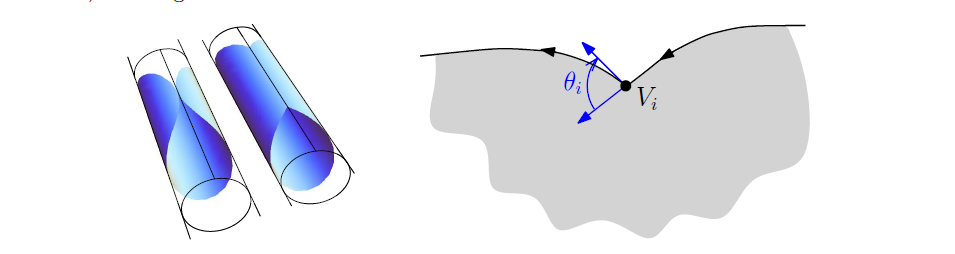
\includegraphics[scale=0.8]{images/angle.png}
        \caption{区域$D_r$的边界.}
        \label{angle}
    \end{figure}
    我们这里选取的定向使得$-\pi \le \theta_i \le 0$.  记$l(r)=l(\P D_r)$. 则由第一变分公式(非光滑点附近需要单独处理, 参考\cite{White}及\cite{Perez}),
    \begin{equation}
        l'(r)=\int_{\P D_r}K_{\P D}ds+2\sum \tan(\frac{\theta_i}{2}).
    \end{equation}
    而由于$\tan(\frac{\theta_i}{2}) \le \frac{\theta_i}{2}$, 及Gauss-Bonnet公式(分段光滑区域上的Gauss-Bonnet公式参考\cite{lee}),
    \begin{equation}
        l'(r)\le \int_{\P D_r}K_{\P D}ds+\sum \theta_i = 2\pi\chi(D_r)-\int_{D_r}Kdv_g.
    \end{equation}
    由于$\mathop{\limsup} l'(r) \ge 0$(若$ \mathop{\limsup l'(r)} \le \alpha <0$, 则存在$r$足够大使得$l(r) < 0$, 这是不可能的), 则有
    \begin{equation} \label{basic_inequality}
        \begin{split}
            0 &\le \limsup_{r\to \infty} l'(r) \le \limsup(2\pi \chi(D_r) - \int_{D_r}Kdv_g) \\
            & \le \limsup (2\pi(2-2p(D_r)-(\P D_r)^\#)-\int_{D_r}K^+dv_g+\int_{D_r}K^-dv_g)
        \end{split}
    \end{equation}
    其中, $p$为$D_r$的亏格, $(\P D_r)^\#$为$D_r$的边界的连通分支数. 上述不等式意味着, 存在常数$C$使得
    \begin{enumerate}
        \item $p(D_r), (\P D_r)^\#, \int_{D_r}K^+dv_g \le C(\int_\Sigma K^-dv_g +1)$. \label{finite}
        \item 存在$r_0>0$使得$\forall r > r_0$, $p(D_r) = p(D_{r_0})$. \label{genus}
    \end{enumerate}
    结论\eqref{finite}由\eqref{basic_inequality}取极限直接得到. 结论\eqref{genus}是因为$p(D_r)$是有上界的, 且$p(D_r)$只取整数值且关于$r$是非减的. 现在, 对于$\Sigma - D_r$,我们证明
    \begin{claim}
        设$r > r_0$, 则$\Sigma - D_r$的每一个紧的连通分支都是单连通的.
        \begin{subproof}
            设$\Omega$是$\Sigma - D_r$的一个连通分支. 若$\P \Omega$至少包含两个边界, 由于$\P \Omega \subset \P D_r$, 则$p(D_r \cup \Omega) > p(D_r)$, 这与结论\eqref{genus}矛盾. 断言证毕.
        \end{subproof}
    \end{claim}
    \par 现在, 记$A_r=D_r\cup \{\Sigma - D_r\text{的所有紧连通分支}\}$. 同时取$r_i$使得\eqref{basic_inequality}成立并且
    \begin{equation} \label{boundary_constant}
        (\P D_{r_i})^\# = (\P D_{r_{i+1}})^\#=c.
    \end{equation}
    $(\P D_{r})^\#$总是取整数值并且有上界, \eqref{boundary_constant}是可以取到的. 由于$(\P A_{r_i})^\# \le (\P D_{r_i})^\#$, 可设
    \begin{equation}
        (\P A_{r_i})^\# = (\P A_{r_{i+1}})^\#=c'.
    \end{equation}
    此时, $A_{r_i} \subset A_{r_{i+1}}$并且 $A_{r_i}$与$A_{r_{i+1}}$同胚, 则$A_{r_{i+1}}$是由$A_{r_i}$在边界处添加annulus而得到. 由于$\Sigma = \cup A_{r_i}$, 则$\Sigma$与 $A_{r_i}$具有相同的拓扑型. 现在可以在不等式\eqref{basic_inequality}可以得到,
    \begin{equation}
        \begin{split}
            0 & \le \limsup (2\pi(2-2p(D_r)-(\P D_r)^\#)-\int_{D_r}K^+dv_g+\int_{D_r}K^-dv_g) \\
            &\le  \limsup (2\pi(2-2p(A_r)-(\P A_r)^\#)-\int_{A_r}Kdv_g) \\
            & \to  2\pi \chi(\Sigma) - \int_\Sigma K dv_g.
        \end{split}
    \end{equation}
    至此, 我们已经证明了$\Sigma$是有限型曲面, 即同胚于闭区曲面去掉有限个点.
    \par 设$E$为$\Sigma$的一个末端 (end, 即$\Sigma-D_{r_0}$的一个连通分支, $r_0$取足够大). 则$E$是annulus. 
    \begin{claim}
        $E$共形同构于$\{1 < \abs{z} < +\infty\}$.
        \begin{subproof}
            记$\Gamma_r=\P D_r \cap E$. 设$\phi: E \to \{ 1 < \abs{z} < R\}$是共形等价. 我们需要证明$R=+\infty$. 设$\Gamma_r(s)$是其弧长参数化. 则
            \begin{equation}
                2\pi = l_{\S^1} \le l_{\phi\circ \Gamma_r} = \int_{\Gamma_r} \abs{d \phi(\Gamma_r)\Gamma'_r}ds.
            \end{equation}
            由Cauchy不等式, 则有
            \begin{equation}
                \begin{split}
                    4\pi^2 \le (\int_{\Gamma_r} \abs{d\phi(\Gamma_r)\Gamma'_r}ds)^2 & \le l_{\Gamma_r}\int_{\Gamma_r}\abs{D\phi(\Gamma_r)}^2ds \\
                    & =l(\Gamma_r)\int_{\Gamma_r}\det \phi ds.
                \end{split}
            \end{equation}
            (最后一个等式中, 我们用到了对于全纯函数$\phi$, $\abs{d\phi}^2 = \abs{\phi'}^2= \det \phi$). 由于
            \begin{equation}
                l'(r) \le 2\pi\chi(D_r) - \int_{D_r}Kdv_g \to 2\pi\chi(\Sigma) - \int_\Sigma K dv_g,
            \end{equation}
            则存在常数$C$使得 
            \begin{equation}
                l(r) \le Cr.
            \end{equation}
            综合以上几个不等式, 我们得到
            \begin{equation}
                \frac{4\pi^2}{Cr} \le \frac{4\pi^2}{l(r)} \le \frac{4\pi^2}{l_{\Gamma_r}} \le \int_{\Gamma_r}\det\phi ds.
            \end{equation}
            对$r$积分, 则有
            \begin{equation}
                \begin{split}
                    +\infty = \int^\infty_{r_0} \frac{4\pi^2}{Cr} &\le \int^\infty_{r_0}\int_{\Gamma_r} \det\phi dsdr  \\
                    &=\Area(\phi(E)) \\
                    &= \Area(\{1<\abs{z}< R\}) 
                \end{split}
            \end{equation}
            因此, $R=+\infty$, 断言证毕.
        \end{subproof}
    \end{claim}
    现在设$\Sigma$是极小曲面, 我们计算$\Sigma$的全曲率.  由命题\eqref{pullback_gauss}可知,
    \begin{equation}
        \int_\Sigma K dv_g = - \Area(N(\Sigma)).
    \end{equation}
    $N$为Gauss映射. 等式右侧面积的计算需要计象集中每个点的重数. 现在, 我们需要说明存在一个整数重数. 
    \begin{claim}
        设$\Sigma$共形等价于$\mathcal{S}-\{p_i\}$, $\mathcal{S}$是闭黎曼曲面.  则其Gauss映射$g: \Sigma\to \overline{\mathbb{C}}$可以延拓为$\mathcal{S}$上的亚纯函数.
        \begin{subproof}
            取$p \in \{p_i\}$, 并取$p$点的邻域, 设这个领域共形等价于$\D^*=\D - \{0\}$. 现在, 可以将$g$看作$g: \D^* \to \overline{\mathbb{C}}$. 设$\gamma_\rho=\{\abs{z}=\rho\}$, 并取$\gamma_\rho$的弧长参数化. 则有
            \begin{equation}
                \abs{l_{g(\gamma_\rho)}}^2 = (\int_{\gamma_\rho} \abs{dg(\gamma_\rho) \gamma'_\rho(s) ds})^2 \le 2\pi\rho \int_{\gamma_\rho}\abs{dg(\gamma_\rho)}^2ds.
            \end{equation}
            两侧同时除以$\frac{1}{2\pi\rho}$并对$\rho$积分, 则有
            \begin{equation}
                \begin{split}
                    \int^1_0 \frac{l^2(g(\gamma_\rho))}{2\pi\rho} d\rho \le \int^1_0 \int_{\gamma_\rho} \abs{dg(\gamma_\rho)}^2dsd\rho &= 2\Area(g(\D^*))  \\
                    &\le -2\int_\Sigma Kdv_g<\infty.
                \end{split}
            \end{equation}
            最后一个不等式是因为命题\eqref{pullback_gauss}. 由于$\frac{1}{\rho}$不可积, 则存在$\rho_i \to 0$使得  $l(g(\rho_i)) \to 0$. 这意味着$g$在0点的邻域内有界. 因此, $g$可以延拓为$\mathbb{D}$上的亚纯函数. 断言得证.
        \end{subproof}
    \end{claim}
    \par  由于黎曼面之间的共形映射是覆盖映射(除去有限个分歧点), 则
    \begin{equation}\label{total_curvature_degree}
        \int_\Sigma Kdv_g = - \text{deg}(g) \Area(\S^2) = -\text{deg}(g)4\pi.
    \end{equation}
\end{proof}
\begin{remark}
    上面等式\eqref{total_curvature_degree}实际上提供了一种计算完备极小曲面全曲率的方法: 只需要知道Gauss映射下$\S^2$上任意一个点的原像的个数, 乘以$4\pi$即可.
\end{remark}
\begin{corollary}\label{flatness_4pi}
    设$\Sigma$是完备的定向极小曲面, 且$-4\pi < \int_\Sigma K dv_g \le 0$, 则$\Sigma$是平面.
\end{corollary}
\begin{proof}[定理\eqref{curvature_estimate_4pi}的证明]
    所有的计算都是在曲面的内蕴度量下进行的. 假设结论不成立. 设$\forall k$, 存在$\Sigma_k$使得$\int_\Sigma \abs{\II_k}^2dv_g \le C$并且存在$p_k \subset \Sigma_k$使得$d(p_k,\P \Sigma_k)\abs{\II_k(p_k)} \to +\infty$. 不失一般性, 我们选择$p_k$使得
    \begin{equation}
        d(p_k, \P \Sigma_k)\abs{\II(p_k)} \ge d(x,\P \Sigma_k)\abs{\II(x)} \s \forall x \in \Sigma_k.
    \end{equation}
    将$p_k$平移到0点处, 将作伸缩$x \to \II_k(p_k)x$, 得到的新的曲面仍记为$\Sigma_k$. 在绅缩变换下,  $\int_{\Sigma_k}\abs{\II}^2dv_g, d(p_k,\P \Sigma)\abs{\II}(p_k)$都是不变的.  因此,这些新的曲面满足
    \begin{equation} \label{iikk0}
        \int_{\Sigma_k} \abs{\II_k}^2 \le C, \s \II_k(0) =1.
    \end{equation}
    特别地, 有$d(0,\P \Sigma_k) \to \infty$以及$d(x,\P \Sigma_k) \abs{\II(x)} \le d(0,\P \Sigma_k)$. 设$x \in B(0,r)$, 则有
    \begin{equation}
        \abs{\II_k(x)} \le \frac{d(0,\P \Sigma_k)}{d(x,\P \Sigma_k)} \le \frac{d(0,\P \Sigma_k)}{d(0,\P \Sigma_k) - d(0,x)} \to 1.
    \end{equation}
    因此, $\abs{\II_k}$局部一致有界. 由定理\eqref{compactness}, 存在极小曲面$\Sigma$, 使得$\Sigma_k \to \Sigma$. 显然地, $\Sigma$是完备的.  并且
    \begin{equation} \label{II01}
        \abs{\II_\Sigma(0)}=1.
    \end{equation}
    另外, 有
    \begin{equation}
        \int_\Sigma \abs{\II_\Sigma}^2dv_g \le \liminf \int_{\Sigma_k} \abs{\II_k}^2dv_g \le C < 8\pi.
    \end{equation}
    这等价于$-\int_\Sigma K dv_g < 4\pi$. 由推论\eqref{flatness_4pi}可知, $\Sigma$是平面, 而这与\eqref{II01}矛盾.
\end{proof}
对于极小曲面$\Sigma^{n-1} \subset \R^n$, 记$\theta(\Sigma,p,R)=\frac{\Area(B(p,R))\cap \Sigma}{\pi R^2}$. 由单调性公式可知, $\theta$关于$R$单调递增且$\mathop{\lim}_{R\to 0} \theta=1$.
\begin{lemma}\label{theta_flat}
    设$\Sigma^{2}\subset \R^3$是极小曲面. 则$\theta \eq 1$当且仅当$\Sigma$是平面.
\end{lemma}
\begin{theorem}
    存在$\lambda >1, \epsilon>0$及$C< \infty$使得如果$\Sigma^2\subset \R^3$是极小曲面, $p\in \Sigma$, $B(p,R) \cap \P \Sigma = \emptyset$且$\theta(\Sigma, p, R) \le \lambda$, 则$\forall x\in  B(p, \epsilon R)$,
    \begin{equation}
        \abs{\II(x)}d(x,\P B(p,\epsilon R)) \le C.
    \end{equation}
\end{theorem}
\begin{proof}
    设论不成立. 取$\lambda_k \to 1, \epsilon_k \to 0$, 则$\forall k$, 存在$\Sigma_k$及$p_k \subset \Sigma_k$, $R_k >0$使得
    \begin{equation}
        \mathop{\sup}_{x \in B(p_k,\epsilon_k R_k)}\abs{\II_k(x)} d(x, \P B(p_k,\epsilon_k R_k)) \to \infty.
    \end{equation}
    设$\abs{\II_k(x)}d(x, \P B(p_k,\epsilon_k R_k))$在$q_k$处取到最大, 则$q_k$是$B(p_k, \epsilon_k R_k)$的内点. 将$q_k$平移到原点处, 并做绅缩$x \to \abs{\II_k(q_k)}d(q_k,\P B(p_k, \epsilon_k R_k))x$. 绅缩变换后得到的极小曲面仍记为$\Sigma_k$. 则
    \begin{equation}
        \abs{\II_k(0)}=1,\s d(0, \P B(p_k, \epsilon_k R_k)) \to \infty.
    \end{equation}
    特别地, 有$R_k \to \infty$.  而$\abs{\II_k(x)} \le \frac{d(0, \P B(p_k, \epsilon_k R_k))}{d(x, \P B(p_k, \epsilon_k R_k))} \to 1$, 则$\abs{\II_k}$局部一致有界. 因此, 存在子列, 仍记为$\Sigma_k$及完备极小曲面$\Sigma$使得$\Sigma_k \to \Sigma$. 而对于任意$R>0$, 由单调性公式,
    \begin{equation}\label{II011}
        \theta(\Sigma,0, R)= \lim_{k \to \infty} \theta(\Sigma_k,0,R) \le \lim_{k\to \infty} \theta(\Sigma_k,0,\frac{1}{1+\epsilon_k}R_k).
    \end{equation}
    另外, 由于$p_k \in B(0, \epsilon_k R_k)$,
    \begin{equation}
        \begin{split}
            \theta(\Sigma_k,0,\frac{1}{1+\epsilon_k}R_k) &=\frac{(1+\epsilon_k)^2}{\pi R_k^2}\Area(B(0,\frac{1}{1+\epsilon_k}R_k)\cap \Sigma_k) \\
            &\le \frac{(1+\epsilon_k)^2}{\pi R_k^2}\Area(B(p_k,R_k)\cap \Sigma_k) \\
            &\le (1+\epsilon_k)^2\lambda_k \to 1.
        \end{split}
    \end{equation}
    则$\theta(\Sigma,0, R) =1$. 由引理 \eqref{theta_flat}可知, $\Sigma$是平面,这与 \eqref{II011}矛盾.
\end{proof}
\section{$L^p$估计}
\begin{theorem} \label{ssy}
    设$\Sigma^{n-1}\subset \R^n$是定向的稳定极小曲面. 则$\forall p \in [2, 2+\sqrt{\frac{2}{n-1}})$, 存在$C=C(n,p)$使得$\forall \phi \in C^1_0(\Sigma), \phi \ge 0$, 成立 
    \begin{equation}
        \int_\Sigma \abs{\II}^{2p}\phi^{2p}dv_g \le C(n,p) \int_\Sigma \abs{\nabla_\Sigma \phi}^{2p}dv_g.
    \end{equation}
\end{theorem}
\begin{proof}
    $\forall f \in C^1_0(\Sigma)$, 取$\eta=\abs{\II}^{1+q}f$代入到稳定性不等式中, 则有
    \begin{equation} \label{ssy1}
        \begin{split}
            \int \abs{\II}^{4+2q}f^2  \le& \int \abs{\nabla_\Sigma (\abs{\II}^{1+q}f)}^2 \\
            =& \int \abs{\II}^{2+2q} \abs{\nabla_\Sigma f} + (1+q)^2 \abs{\II}^{2q}f^2 \abs{\nabla \abs{\II}}^2  \\
            &+ 2(1+q)\abs{\II}^{2q+1}f\inner{\nabla_\Sigma \abs{\II}}{\nabla_\Sigma f}.
        \end{split}
    \end{equation}
    由Simons不等式,
    \begin{equation}
        \abs{\II}\Delta_\Sigma\abs{\II} + \abs{\II}^4 \ge \frac{2}{n-1}\abs{\nabla_\Sigma \abs{\II}}^2.
    \end{equation}
    两侧同时乘以$\abs{\II}^{2q}f^2$并积分后应用散度定理, 则有
    \begin{equation} \label{ssy2}
        \begin{split}
            \frac{2}{n-1}\int \abs{\nabla_\Sigma \abs{\II}}^2 \abs{\II}^{2q}f^2 \le&  \int \abs{\II}^{2q+4}f^2 + \Delta_\Sigma \abs{\II} \abs{\II}^{2q+1}f^2 \\
            =&\int \abs{\II}^{2q+4}f^2-\inner{\nabla_\Sigma \abs{\II}}{\nabla_\Sigma}\\
            =&\int \abs{\II}^{2q+4}f^2-2f\abs{\II}^{2q+1}\inner{\nabla_\Sigma \abs{\II}}{\nabla_\Sigma f}\\
            &-(2q+1)f^2\abs{\II}^{2q} \abs{\nabla_\Sigma\abs{\II}}^2.
        \end{split}
    \end{equation}
    将不等式\eqref{ssy1}与\eqref{ssy2}相加后, 得到
    \begin{equation}
        \begin{split}
            &(\frac{2}{n-1}-q^2)\int\abs{\nabla_\Sigma \abs{\II}}^{2q} \abs{\II}^2 f^2 \\
            \le & \int \abs{\II}^{2+2q}+2q\abs{\II}^{2q+1}f\inner{\nabla_\Sigma \abs{\II}}{\nabla_\Sigma f} \\
            \le& \int \abs{\II}^{2+2q}\abs{\nabla_\Sigma f}^2 + 2q(\frac{1}{\epsilon}q^2 \abs{\nabla_\Sigma f}^2 + \epsilon f^2 \abs{\nabla_\Sigma \abs{\II}})\abs{\II}^{2q}. 
        \end{split}
    \end{equation}
    因此, 我们有
    \begin{equation} \label{ssy3}
        (\frac{2}{n-1}-q^2-2q\epsilon) \int \abs{\nabla \abs{\II}}^{2q} \abs{\II}^2 f^2 \le (1+2q\epsilon)\int \abs{\II}^{2+2q}\abs{\nabla_\Sigma}^2.
    \end{equation}
    这里, 要求
    \begin{equation}
        \frac{2}{n-1}-q^2 >0.
    \end{equation}
    将不等式\eqref{ssy3}代入到\eqref{ssy1}中, 则有
    \begin{equation}
        \begin{split}
            \int \abs{\II}^{4+2q}f^2 &\le 2(\int \abs{\II}^{2+2q}\abs{\nabla f}^2 + (1+q)^2f^2\abs{\II}^{2q}\abs{\nabla_\Sigma \abs{\II}}^2) \\
            & \le 2(1+\frac{1+2q\epsilon}{\frac{2}{n-1}-q^2-2q\epsilon}(1+q)^2)\int \abs{\II}^{2+2q}\abs{\nabla_\Sigma f}^2.
        \end{split}
    \end{equation}
    取$q=p-2, f=\phi^p$, 应用H\"older不等式, 则有
    \begin{equation}
        \begin{split}
            \int \abs{\II}^{2p} \phi^{2p} &\le C(n,p)\int \abs{\II}^{2p-2}\phi^{2p-2}\abs{\nabla_{\Sigma}\phi}^2 \\
            & \le C(n,p)(\int\abs{\II}^{2p}\phi^{2p})^\frac{p-1}{p}(\int\abs{\II}^{2p})^{\frac{1}{p}}.
        \end{split}
    \end{equation}
\end{proof}
\begin{theorem}
    设$\Sigma^{n-1} \subset \R^n$是完备, 定向, 稳定的极小曲面. 设$n \le 6$且存在$C>0$ 使得
    \begin{equation}
        \Area(B_r\cap \Sigma) \le Cr^{n-1}.
    \end{equation}
    则$\Sigma$是平坦的.
\end{theorem}
\begin{proof}
    设$\rho>0$. 设$\phi$是$B_{2\rho}, B_\rho$上的截断函数, 且$\abs{\nabla \phi}\le \frac{2}{\rho}$. 取$p$满足
    \begin{equation}
        \frac{n-1}{2} < p \s \text{且}\s 2\le p < 2+\sqrt{\frac{2}{n-1}}.
    \end{equation}
    $n\le 6$时这样的$p$是存在的. 代入到定理\eqref{ssy}中, 则有
    \begin{equation}
        \begin{split}
            \int_{B_\rho\cap \Sigma} \abs{\II}^{2p} &\le C(n,p)\frac{1}{\rho^{2p}}\Area(B_{2\rho})\\
            &\le C(n,p)\rho^{n-1-2p} \overset{\rho \to \infty}{\longrightarrow} 0.
        \end{split}
    \end{equation}
\end{proof}
\chapter{粘性解}
\section{粘性解与非线性方程}
在本章中, 如无特殊说明, 我们考虑的是单位球$B_1$中方程
\begin{equation}\label{vis_eq}
    \L u=\aij(x)\dij u(x)= f(x)
\end{equation}
这是, 我们假设$\aij$满足$(\lambda, \Lambda)$一致椭圆条件且$\aij, f \in C(B_1)$.  
%粘性解是一种非常弱意义下的解, 它的提出基于最大值原理, 并且适用于完全非线性方程.  
\begin{theorem}[最大值原理]
    设$u \in C^2$, $\Delta u \ge 0$, 则 $\max_\O u=\max _{\partial \O} u$.  
\end{theorem}
从另一个角度来看最大值原理:设$u \in C^2$, $\Delta u \ge 0$.  设$ \phi \in C^\infty $使得在$x_0$处, $\phi(x_0)=u(x_0)$.  在$B_\epsilon(x_0)$中, $u(x) \le \phi(x)$.  则 $\Delta \phi(x_0) \ge 0$.  因为显然, $u-\phi$在$x_0$处取到局部最大值.  若$\Delta \phi <0$, 则$\Delta(u-\phi) >0$, 这意叶着$x_0$处$u-\phi$不可能是局部最大值.  
\par 从这个角度来看, $u \in C^2$的条件是不需要的.  另外算子$\Delta$所起到的作用也只是算子 $\Delta$具有最大值原理.  
\begin{definition} \label{def_viscosity}
    称$u \in C(\O)$是方程$\L u=f$的粘性上解, 如果$\forall x_0 \in \O$及 $\phi \in C^2(\O)$, 假如$u-\phi$在$x_0$处取到局部最小值, 则$\L \phi(x_0) \le f(x_0)$.  
\end{definition}
若$u-\phi$在$x_0$处取到局部最小值, 记为$a$.  则在$x_0$的邻域中, $u\ge \phi+a$.  因此, $\L(\phi+a)(x_0)=\L (\phi)(x_0) \le f(x_0)$.  因此, 上解的一个等价定义是: 
\begin{definition}
若对于任意可以从下侧在$x_0$处接触$u$的函数$\phi \in C^2$, 都有$\L\phi (x_0) \le f(x_0)$, 则称$u$是方程$\L u=f$的粘性上解.  
\end{definition}
    类似地, 可以定义粘性下解.  若$u$同时是粘性上解与粘性下解, 则称$u$是粘性解.  
\begin{remark}
    上面的定义中, 我们没有用到任何关于$L$的线性性质.  由于非线性椭圆方程也具有最大值原来, 因此粘性解的定义可以方便地推广到非线性方程.  
\end{remark}
\begin{definition}
    设$\S$是实对称矩阵的集合.  设$F: S\times \O \to \R$连续.  称$F$是一致椭圆的, 如果存在$\lambda, \Lambda>0$使得 $\forall M \in \S$及半正定矩阵$N$, $\forall x \in \O$, 成立
    \begin{equation}
        \lambda \norm{N}\le F(M+N, x)-F(M, x) \le \Lambda\norm{N}
    \end{equation}
\end{definition}
与定义\eqref{def_viscosity}完全相同的方法, 我们可以定义完全非线性方程 
\begin{equation*}\label{vis_nonlinear_eq}
    F(D^2u, x)=f
\end{equation*}
的粘性解.  
\begin{remark}
    根据一致椭圆的定义, 
    \begin{equation*}
        \lambda \norm{N} \le F(M+N, x) -F(M, x) < \Lambda \norm{N}, \s \forall N \ge 0.  
    \end{equation*}
    而如果$N$只是对称矩阵, 记 $N=N^+-N^-$.  其中, $N^+, N^-$都是半正定矩阵.  由谱定理可知, 这样的分解是存在的且是唯一的.  则
    \begin{equation}
        \begin{split}
            F(M+N, x)= & F(M+N^+-N^-, x)  \\
            \le &F(F+N^+, x)-\lambda \norm{N^-} \\
            \le &F(M, x)+\Lambda \norm{N^+}-\lambda\norm{N^-}
        \end{split}
    \end{equation}
    如果上面的不等式成立, 显然$F$是一致椭圆的.  
\end{remark}
\begin{proposition}
    下面的叙述是等价的.  
    \begin{enumerate}
        \item \label{t1} $u$是方程$F(D^2u, x)=f$的粘性上解.  
        \item \label{t2} 对于任意$C^2$函数$\phi$, 如果$\phi$在$x_0$处从下方接触$u$, 则
        \begin{equation*}
            F(D^2\phi(x_0), x_0)\le f(x_0).  
        \end{equation*}
        \item \label{t3} 对于任意二次多项式$\phi$, 如果$\phi$在$x_0$处从下方接触$u$, 则
        \begin{equation*}
            F(D^2\phi(x_0), x_0)\le f(x_0).  
        \end{equation*}
    \end{enumerate}
\end{proposition}
\begin{proof}
    \eqref{t1} $\iff$ \eqref{t2} $\implies$ \eqref{t3}是显然的.  \\
    \eqref{t3} $\implies$ \eqref{t2}: 设$\phi \in C^2(\O)$, 且在$x_0$处从下方接触$u$.  记
    \begin{equation}
        p_\epsilon(x)=\phi(x_0)+D\phi(x_0)(x-x_0)+D^2\phi(x_0)(x-x_0)^2 -\epsilon\abs{x-x_0}^2
    \end{equation}
    显然, $p_\epsilon$在$x_0$处从下方接触$u$.  因此 
    \begin{equation}
        F(D^2p_\epsilon(x_0), x_0)=F(D^2\phi(x_0)-2\epsilon I, x_0) \le f(x_0).  
    \end{equation}
    令$\epsilon \to 0$即可.  
\end{proof}
\begin{proposition}
    若$u \in C^2(\O)$.  则$u$是方程\eqref{vis_nonlinear_eq}的粘性上解, 当且仅当$u$是方程\eqref{vis_nonlinear_eq}的经典上解, 即$F(D^2u, x) \le f(x)$逐点成立.  
\end{proposition}
\begin{proof}
    设$u$是粘性上解.  固定$x_0\in \O$.  记
    \begin{equation}
        p_\epsilon(x)=u(x_0)+Du(x_0)(x-x_0))+D^2u(x_0)(x-x_0)^2-\epsilon\abs{x-x_0}^2.  
    \end{equation}
    显然, $p_\epsilon(x)$在$x_0$处从下方接触$u$.  因此有
    \begin{equation}
        F(D^2p_\epsilon(x_0), x_0)=F(D^2u(x_0)-2\epsilon I, x_0) \le f(x_0).  
    \end{equation}
    令$\epsilon\to 0$即可.  
    \par 反之, 设$u$是经典解.  若$\phi$在 $x_0$处从下方接触$u$, 则$u - \phi$在$x_0$处取到局部最小值.  因此, $D^2(u-\phi)(x_0) \ge 0$.  则由$F$的一致椭圆性质, 
    \begin{equation}
        F(D^2\phi, x_0) \le F(D^2\phi+D^2(u-\phi), x_0)=F(D^2u, x_0) \le f(x_0)
    \end{equation}
\end{proof}
\begin{proposition}
    若$u, v$是$F(D^2u, x)=f(x)$的粘性上解, 则$\min(u, v)$也是粘性上解.  
\end{proposition}
\begin{proof}
    由定义可知.  
\end{proof}
\begin{theorem}[粘性解的稳定性]
    设$F_k: \S \times \O \to \R$是$(\lambda, \Lambda)$一致椭圆的.  设$u_k$是方程$F_k(D^2u, x)=f(x)$的粘性上解.  设 $F_k \to F$内闭一致, 且$u_k \to u$内闭一致.  则 $u$是方程$F(D^2u, x)=f(x)$的粘性上解.  
\end{theorem}
\begin{proof}
    在$x_0$处, 设$\phi$是从下方接触$u$的抛物面.  设在$\overline{B}_r(x_0)$中, $\phi(x) \le u(x)$.  则当$\epsilon>0$足够小时, $\phi_\epsilon=\phi-\epsilon\abs{x-x_0}^2$从下方接触$u$, 且在$\overline{B}_r(x_0)-\{x_0\}$上, $\phi_\epsilon < u(x)$.  $\forall k\in N^+$, 设$a_k = \min_{\overline{B}_r(x_0)}(u_k-\phi_\epsilon)$, 且最小值在$x_k$点处取到.  显然, 
    \begin{equation}
        \phi_\epsilon + a_k \le u_k
    \end{equation}
    另外, 由于$u_k \to u$内闭一致, 则 
    \begin{equation}
        a_k \to \min_{\overline{B}_r(x_0)}(u-\phi_\epsilon)=0.  
    \end{equation}
    另外, 若$x_k \to \tilde{x}_0$, 则
    \begin{equation}
        (u_k-\phi_\epsilon)(x_k) \to (u-\phi_\epsilon)(\tilde{x}_0)
    \end{equation}
    而由于$u-\phi_\epsilon$在$B_r(x_0)$中只在$x_0$处取到最小值, 则$x_0=\tilde{x}_0$.  选取一个子列后, $\phi_\epsilon+a_k$在$x_k$处从下方接触$u_k$.  于是
    \begin{equation}
        F(D^2(\phi_\epsilon), x_k) \le f(x_k)
    \end{equation}
    令$k \to \infty$, 则$F(D^2\phi_\epsilon, x_0) \le f(x_0)$.  令$\epsilon \to 0$, 则$f(D^2\phi, x_0) \le f(x_0)$.  证毕.  
\end{proof}
\section{椭圆方程解的集合:\texorpdfstring{$\S$}{S}类}
设$u \in C^2(\O)$是方程$\aij D_{ij}u=f$的上解, 则有
\begin{equation}
    \begin{split}
        \tr (AD^2u) \le f \implies& tr(OAO^T, diag(\lambda_i)) \le f \\
        \implies & \Sigma \tilde{a}^{ii}\lambda_i \le f \\
        \implies & \lambda \Sigma_{\lambda_i >0} \lambda_i + \Lambda \Sigma_{\lambda_i <0} \lambda_i \le f
    \end{split}
\end{equation}
其中, $\tilde{a}^{ij}=(OAO^T)^{ij}$, $O$是将$D^2u$对角化的标准正交矩阵, $\lambda_i$是$D^2u$的特征值.  同样的, 若$u$是$\aij D_{ij}u=f$的下解, 则
\begin{equation}
     \Lambda \Sigma_{\lambda_i >0} \lambda_i + \lambda \Sigma_{\lambda_i <0} \lambda_i \ge f
\end{equation}
\begin{definition}
    设$S_{\lambda, \Lambda}$是所有特征值在$(\lambda, \Lambda)$之间的正定矩阵的集合.  $\forall M \in \S$, 设$\{\lambda_i\}$是$M$的特征值.  定义算子
    \begin{equation}
        \begin{split}
            \mathcal{M}^+(M)= \MP{M} = &\Lambda \Sigma_{\lambda_i>0}\lambda_i+\lambda\Sigma_{\lambda_i<0}\lambda_i  \\
            = &\sup_{A\in \S_{\lambda, \Lambda}}\tr(AM)
        \end{split}
    \end{equation}
    \begin{equation}
        \begin{split}
            \mathcal{M}^-(M)= \MN{M} = &\lambda \Sigma_{\lambda_i>0}\lambda_i+\Lambda\Sigma_{\lambda_i<0}\lambda_i  \\
            = &\inf_{A\in \S_{\lambda, \Lambda}}\tr(AM)
        \end{split}
    \end{equation}
\end{definition}
显然, 由定义可知
\begin{proposition} \label{property_m}
    $\forall M, N \in \S$, 成立
    \begin{equation}
        \MN{M}+\MN{N}\le \MN{M+N}
    \end{equation}
    \begin{equation}
        \MP{M+N} \le \MP{M} + \MN{N}
    \end{equation}
\end{proposition}
现在, 我们定义“所有上解的集合”与“所有下解的集合”.  
\begin{definition}
    设$f$连续, $\O$有界, $0< \lambda < \Lambda$.  称$u \in \SSP{f}$, 如果$\forall  x_0 \in \O$及任意从下方接触$u$的$C^2$函数$\phi$, 成立
    \begin{equation}
        \lambda \Sigma_{\lambda_i >0} \lambda_i + \Lambda \Sigma_{\lambda_i <0} \lambda_i \le f(x_0)
    \end{equation}
    其中, $\lambda_i$是$D^2\phi(x_0)$的特征值.  \\
    称$u \in \SSN{f}$, 如果$\forall  x_0 \in \O$及任意从上方接触$u$的$C^2$函数$\phi$, 成立
    \begin{equation}
        \Lambda \Sigma_{\lambda_i >0} \lambda_i + \lambda \Sigma_{\lambda_i <0} \lambda_i \ge f(x_0)
    \end{equation}
\end{definition}
记$\SS{f}=\SSP{f} \cap \SSN{f}$.  
\begin{proposition}
    若$u \in C^2(\O)$.  则$u \in \SSP{f}$当且仅当 $\forall x \in \O$, 存在正定矩阵$\aij$使得 $\aij$的特征值在$[\lambda, \Lambda]$之间且$\aij D_{ij}u(x) \le f(x)$.  
\end{proposition}
\begin{proof}
    略.  
\end{proof}
\begin{remark}
    上面的命题中得到的$\aij$关于$x$当然不一定是连续的.  
\end{remark}
\begin{proposition} \label{ppp1}
    设$u$是方程$F(D^2u, x) = f(x)$的粘性上解, $F$满足$(\lambda, \Lambda)$一致椭圆条件.  则$u \in \S^+(\frac{\lambda}{n}, \Lambda, f(x)-F(0, x))$.  并且$\forall \psi \in C^2(\O)$, 成立 
    \begin{equation}
        u-\psi \in \S^+(\frac{\lambda}{n}, \Lambda, f(x)-F(D^2\psi, x))
    \end{equation}
\end{proposition}
\begin{proof}
    设$\psi \in C^2(\O)$.  设$\phi \in C^2(\O)$在点$x_0$处从下方接触$u-\psi$.  则$\phi+\psi$在$x_0$处从下方接触$u$.  于是
    \begin{equation}
        F(D^2\phi+D^2\psi, x_0) \le f(x_0)
    \end{equation}
    另外, 由一致椭圆性, 有
    \begin{equation}
        F(D^2\psi, x_0) + \lambda\norm{D^2\phi^+}-\Lambda\norm{D^2\psi^-} \le f(x_0)
    \end{equation}
    又因$\norm{D^2\psi^+}=\max\lambda(D^2\phi)$, $\norm{D^2\psi^-}=\max(-\min\lambda(D^2\phi), 0)$, 则有
    \begin{equation}
        \frac{\lambda}{n}\Sigma_{\lambda_i>0}\lambda_i(D^2\phi)-\Lambda\Sigma_{\lambda_i<0}\lambda_i(D^2\phi) \le f(x_0) - F(D^2\psi, x_0)
    \end{equation}
    因此, $u-\psi \in S^+(\frac{\lambda}{n}, \Lambda, f(x)-F(D^2\psi, x))$.  取$\psi=0$, 则有 
    \begin{equation}
        u\in \S^+(\frac{\lambda}{n}, \Lambda, f(x)-F(0, x))
    \end{equation}
\end{proof}
\section{Alexandroff最大值原理}
%\subsection{法映射与接触集}
这一节我们介绍Alexandroff最大值原理, 也称Alexandroff-Bakelman-Pucci估计, 简称ABP估计.  
\subsection{经典ABP估计}
\begin{definition}
    设$\O\subset \R^n$是有界区域.  设$u \in C(\O)$, $y \in \O$.  记
    \begin{equation}
        \chi(y)=\{p \in \R^n\mid u(x) \le u(y)+\inner{p}{x-y} \s \forall x\in \O\}
    \end{equation}
    称$\chi: \O \to 2^{\R^n}$为$u$所确定的(上)法映射.  
\end{definition}
法映射的几何含义:固定$y \in \O$, 记$z(x)=u(y)+\inner{p}{x-y}$, 那么$z(x)$表示通过点$(y, u(y))$并且“斜率”为$p$的平面(法向量为$(-p, 1)$).  因此, $\chi(y)$表示在$y$点处, 从上方接触$u$的平面的“斜率”.  记
\begin{equation}
    \O_u^+=\{y\in \O \mid \chi(y) \ne \emptyset\}.  
\end{equation}
称$\O_u^+$为$u$的\textit{上接触集}.  显然地, $\O^+_u=\O$当且仅当$u$是凹函数.  另外, 易知若$u \in C^1$, 则$\chi(y)=\emptyset$ 或$\chi(y)=\{Du(y)\}$.  若$u \in C^2$, 则$ \forall y_0 \in \O_u^+$, $D^2u(y_0)\le 0$.  因为此时, 存在仿射映射$L$使得 $u \le L$且$u-L$在$y_0$处取到局部最大值.  因此, $D^2(u-L)(y_0) \le 0$.  \par
同样的方式可以定义$u$的\textit{下接触集}$\O^-_u$.  \par
下面的引理是Alexandroff极大值原理的核心, 它本身与方程无关.  
\begin{lemma}\label{abp_c11}
    设$g \in L^1_{loc}$且$g \ge 0$.  则 $\forall u \in C(\O)\cap C^{1, 1}(\O)$, 有
    \begin{equation}
        \int_{B_{\tilde{M}(0)}}g \le \int_{\O^+_u}g(Du)\abs{\det D^2u}
    \end{equation}
    其中, $\tilde{M}=(\sup_\O u - \sup_{\partial \O}u^+)/d$, $d=diam(\O)$.  
\end{lemma}
\begin{remark}
    若$u$在边界上不连续, 只需将$\sup_{\partial \O}u^+$换为$\limsup_{x \to \partial \O}u^+$即可.  
\end{remark}
\begin{proof}
    不失一般性, 假设$u|_{\partial \O} \le 0$.  此时, $\sup_{\partial \O}u^+=0$.  记$\O^+=\{u >0\}$, 则由面积公式
    \begin{equation}
        \int_{Du(\O_u^+ \cap \O^+)}g \le \int_{\O_u^+\cap \O^+} g(Du) \abs{\det D^2u}
    \end{equation}
    现在, 我们证明下面的断言.  
    \begin{claim*}
        \begin{equation}
            B_{\tilde{M}(0)} \subset Du(\O^+\cap \O^+_u)
        \end{equation}
        即, $\forall \abs{a} \le \tilde{M}, \s \exists  y \in \O^+ \cap \O^+_u$ 使得$a=Du(y)$.  
    \end{claim*}
    设$u$在$x_0$处取到最大值$m$, 即有
    \begin{equation}
        u(x_0)=m=\sup u 
    \end{equation}
    显然, $Du(x_0)=0$.  设$\abs{a} < \tilde{M} = \frac{m}{d}$ 考虑平面$L(x)=m+\inner{a}{x-x_0}$.  由于$\abs{a} < \frac{m}{d}$, 则$L(x)$与$\R^n \times \{0\}$的交集位于$\O$外部, 即 
    \begin{equation}
        \{L(x)=0\} \subset \R^n -\O
    \end{equation}
    将$L(x)$向上平移至恰好与$u$相切, 这个切点记为$y$, 则$Du(y)=a$.  显然, $y \in \O^+_u$且$u(y) \ge 0$.  证毕.  
\end{proof}
\begin{remark}
    根据证明过程, 我们可以用$\O^+_u \cap \{u > \max_{\partial \O}u^+\}$替换结论右侧的$\O^+_u$.  
\end{remark}
\begin{corollary}
    设$u \in C^{1, 1}(\O) \cap C(\overline{\O})$, 有
    \begin{equation}
        \sup_\O u \le \sup_{\P \O} + \frac{d}{\omega_n^{\rec{n}}}(\int_{\O^+_u}\abs{\det D^2u})^\rec{n}
    \end{equation}
    其中, $d=\diam \O$.  
\end{corollary}
\begin{corollary} \label{abp_cor1}
    记$D=\det(\aij)$, $D^*=D^\rec{n}$, 则
    \begin{equation}
        \int_{B_{\tilde{M}(0)}}g \le \int_{\O^+_u}g(Du)(-\frac{\aij D_{ij}u}{D^*})^n
    \end{equation}
\end{corollary}
\begin{proof}
    对于半正定矩阵$A, B$, 有不等式$(\det A \det B)^\rec{n} \le \frac{\tr{AB}}{n}$.  取$A=[\aij], B=-D^2u$, 只需注意到在$\O^+_u$上, $D^2u$是半负定的, 应用引理\eqref{abp_c11}即可.  
\end{proof}
\begin{corollary} \label{abp_cor2}
    设$u \in C^2(\O) \cap C(\overline{\O})$, $\aij D_{ij}u \ge f$.  则
    \begin{equation}
        \sup_\O u \le \sup_{\P \O} u^+ + C\norm{\frac{f^-}{D^*}}_{L^n(\O^+_u)}
    \end{equation}
    其中, $C=C(n, \diam(\O))$.  
\end{corollary}
\begin{proof}
    在$\O^+_u$上, $0 \le -\aij D_{ij}u \le -f \le f^-$, 取$g \eq 1$, 应用推论\eqref{abp_cor1}即可.  
\end{proof}
\begin{theorem}\label{classical_abp}
    设$u \in C(\overline{\O}) \cap C^2(\O)$满足 $Lu= \aij \dij u + b^iD_iu +cu  \ge f$.  设$\aij$可测且满足一致椭圆条件.  记$D=\det \aij$, $D^*=D^\rec{n}$.  假设$L$的系数满足
    \begin{equation}
        \frac{\abs{b}}{D^*}, \frac{f}{D^*} \in L^n(\O), \s c\le 0
    \end{equation}
    则存在常数$C=C(n, \diam(\O), \norm{\frac{b}{D^*}})$ 使得
    \begin{equation}
        \sup_\O u \le \sup_{\O}u^+ + C\norm{\frac{f^-}{D^*}}_{L^n(\O)}
    \end{equation}
\end{theorem}
\begin{proof}
    在推论\eqref{abp_cor1}中, 取 $g(x)=\rec{\abs{x}^n+\mu^n}$, $\mu >0$待定.  在$\O^+_u \cap \O^+$上$(\text{注}\O^+=\{u>0\})$, 
    \begin{equation}
        \begin{split}
            -\aij \dij u \le & b^iD_iu + cu -f \\
            \le & b^iD_iu +f^-\\
            \le &\abs{b}\abs{Du} + \frac{f^-}{\mu}\mu \s (\Holder\text{不等式})\\
            \le &(\abs{b}^n + (\frac{f^-}{\mu})^n)^\rec{n}(\abs{Du}^n+\mu^n)^\rec{n}2^{\frac{n-2}{n}}
        \end{split}
    \end{equation}
    将$g(x)=\rec{\abs{x}^n+\mu^n}$代入并应用推论\eqref{abp_cor1}, 
    \begin{equation}
        \begin{split}
            \int_{B_{\tilde{M}(0)}} \frac{1}{\abs{x}^n+\mu^n} \le & \int_{\O^+_u \cap \O^+} \rec{\abs{Du}^n + \mu^n} \rec{D} (\frac{-\aij \dij u}{n})^n \\
            & \le C(n) \int_{\O^+_u \cap \O^+} \rec{D}(\abs{b}^n \abs{\frac{f^-}{\mu}}^n) \\
            & = C(n)\int_{\O^+_u\O^+}(\abs{\frac{b}{D^*}}^n+\abs{\frac{f^-}{\mu D^*}}^n)
        \end{split}
    \end{equation}
    左侧可以直接用极坐标来计算.  
    \begin{equation}
        \begin{split}
            \int_{B_{\tilde{M}(0)}} \rec{\abs{x}^n+\mu^n} =& \int^{\tilde{M}}_0 \int_{\mathbb{S}^{n-1}}\rec{r^n+\mu^n}r^{n-1}d\mathbb{S}^{n-1}dr \\
            =& \frac{w_n}n\log(\frac{\tilde{M}^n}{\mu^n}+1)
        \end{split}
    \end{equation}
    取$\mu = \norm{\frac{f^-}{D^*}}_{L^n(\O^+_u \cap \O^+)}$, 则有
    \begin{equation}
        \log(\frac{\tilde{M}^n}{\mu^n}+1) \le C(n)(\norm{\frac{b}{D^*}}^n+1).  
    \end{equation}
    因此, 
    \begin{equation}
        \tilde{M}^n \le (\exp (C(n)(\norm{\frac{b}{D^*}}^n_{L^n})+1)-1)\norm{\frac{f^-}{D^*}}^n_{L^n}
    \end{equation}
    则有
    \begin{equation}
        \sup_\O u \le \sup_{\partial \O} u^+ + C(n, d, \norm{\frac{b}{D^*}}_{L^n})\norm{\frac{f^-}{D^*}}_{L^n}
    \end{equation}
\end{proof}
\begin{corollary}
    对于任意$u \in C(\overline{\O})\cap W^{2, n}(\O)$, 定理 \eqref{classical_abp}成立.  
\end{corollary}
\begin{proof}
    记$\O_\delta = \{x \in \O \mid d(x, \partial \O ) > \delta\}$, 记$u_\epsilon$为$u$的标准磨光.  则当$\epsilon  < \delta$时, $u_\epsilon $在$\O_\delta$中是良好定义的, 且$\epsilon \to 0$时, $u_\epsilon \tto{\text{内闭一致且$W^{2, n}$收敛}} u$.  另外, 通过给$u_\epsilon$加上一个常数, 可以假设$u_\epsilon \le u$.  $u_\epsilon$满足
    \begin{equation}
        \begin{split}
            &\aij \dij u_\epsilon + b^iD_iu_\epsilon+cu_\epsilon  \\
            \ge& \aij \dij (u_\epsilon-u)+b^iD_i(u_\epsilon-u)+c(u_\epsilon-u)+f \\
            \ge & \aij \dij(u_\epsilon-u)+b^iD_i(u_\epsilon-u)-f^- \eq F
        \end{split}
    \end{equation}
    则有:
    \begin{equation}
        \sup_{\O_\delta} u_\epsilon\le \sup _{\P \O_\delta} u^+_\epsilon+C\norm{\frac{F^-}{D^*}}_{L^n}
    \end{equation}
    考虑到$\lambda \le D^* \le \Lambda$ 及$u_\epsilon \tto{\text{$W^{2, n}$}} u$, 则有
    \begin{equation}
        \norm{\frac{F^-}{D^*}}_{L^n} \to \norm{\frac{f^-}{D^*}}_{L^n}
    \end{equation}
    因此, 对于任意$\delta >0$, 
    \begin{equation}
        \sup_{\O_\delta} u \le \sup _{\P \O_\delta}u^+ +C\norm{\frac{f^-}{D^*}}_{L^n(\O_\delta)}
    \end{equation}
    令$\delta \to 0$即可.  
\end{proof}
\subsection{粘性解的ABP估计}
\begin{definition}
    称二次多项式$p(x)$是开口为 $M$抛物面, 如果$$p(x)=L(x)\pm\frac{M}{2}\abs{x}^2.  $$  其中, $L(x)$为仿射.  
    \par 给定有界区域$\O \subset \R^n$及 $u \in C(\O)$, 设$A \subset \O$为开集, $x_0\in A$.  定义
    \begin{equation}
        \begin{split}
            \theta^+(u, A)(x_0)= \inf \{
                &M>0 \mid \text{存在抛物面} p(x)=L(x)+\frac{M}{2}\abs{x-x_0}^2 \\
                &\text{使得在$A$中}, p(x) \ge u \text{且} p(x_0)=u(x_0)
                \}
            \end{split}
    \end{equation}
    \begin{equation}
        \begin{split}
            \theta^+(u, A)(x_0)= \inf \{
                &M>0 \mid \text{存在抛物面} p(x)=L(x)-\frac{M}{2}\abs{x-x_0}^2 \\
                &\text{使得在$A$中}, p(x) \le u \text{且} p(x_0)=u(x_0)
                \}
            \end{split}
    \end{equation}
    如果右侧的集合为空, 则定义$\theta^+(u, A)(x_0)(\theta^-(u, A)(x_0))=+\infty$.  \\
    定义 $\theta(u, A)(x_0)=\max(\theta^+(u, A)(x_0), \theta^-(u, A)(x_0)) \in [0, +\infty]$.  
\end{definition}
\begin{remark}
    $\theta^+, \theta^-$表示了一种“单侧可微性”, 例如如果$\theta(u, A)(x_0) < +\infty$, 则 $u$夹在两个相切的抛物面之间, 因此 $u$在$x_0$处是可微的.  
\end{remark}
\begin{lemma}\label{d2u_theta}
    设$p \in (1, +\infty]$, $u \in C(\O)$.  设$\epsilon>0$是固定的常数.  记
    \begin{equation}
        \theta(u, \epsilon)(x)=\theta(u, B_\epsilon(x) \cap \O)(x)
    \end{equation}
    若$\theta(u, \epsilon) \in L^p(\O)$, 则$D^2u$存在且
    \begin{equation}
        \norm{D^2u}_{L^p} \le C(n) \norm{\theta(u, \epsilon)}_{L^p}
    \end{equation}
\end{lemma}
\begin{proof}
    只需证明$\forall \phi \in C^\infty_0$, 
    \begin{equation*}
        \abs{\int_\O u \dij \phi} \le \norm{\theta(u, \epsilon)}_{L^p}\norm{\phi}_{L^{p'}} \s \rec{p}+\rec{p'}=1.  
    \end{equation*}
    记$v=\frac{\sqrt{2}}{2}(e_i+e_j)$, 则$\dij \phi= \rec{2}(2D_{vv}\phi-D_{ii}\phi-D_{jj}\phi)$.  因此, 只需考虑 $i=j$的情况即可.  设$\phi\in C^\infty_0$.  则
    \begin{equation}
        \int_\O u D_{ii} \phi = \lim_{\delta \to 0} \int_\O u \Delta_{\delta e_i} \phi = \lim_{\delta \to 0} \int_\O \Delta^2_{\delta e_i}u \phi
    \end{equation}
    其中, $\Delta^2$是二阶差商
    \begin{equation}
        \Delta^2_hu(x)=\frac{u(x+h)+u(x-h)-2u(x)}{\abs{h}^2}
    \end{equation}
    $\forall x \in \{\theta(u, \epsilon) < +\infty\}$, 存在$p_1(x) = L_1(x)+\frac{M}{2}\abs{x}^2$及$p_2(x)=L_2(x)-\frac{M}{2}\abs{x}^2$使得在$\O \cap B_\epsilon(x)$中, $p_2(x) \le u(x) \le p_1(x)$.  $M > \theta(u, \epsilon)$任意.  因此, 
    \begin{equation}
        \Delta^2_hp_2(x) \le \Delta^2_h u(x) \le \Delta^2_hp_1(x)
    \end{equation}
    则有
    \begin{equation}
        -M \le \Delta^2_hu(x) \le M
    \end{equation}
    于是, 
    \begin{equation}
        \abs{\Delta^2_hu(x)} \le \theta(u, \epsilon)(x)
    \end{equation}
    综上, 有 
    \begin{equation}
        \abs{\int_\O u D_{ii} \phi} \le \norm{\theta(u, \epsilon)}_{L^p} \norm{\phi}_{L^{p'}}
    \end{equation}
\end{proof}
\begin{lemma}\label{c_11}
    设$u \in C(\overline{\O})$且$\O \subset \R^n$是有界区域.  设$\theta(u, \epsilon) \le K$, 则 $\abs{Du(x)-Du(y)} \le C(n)K\abs{x-y}$.  即有$u \in C^{1, 1}(\overline{\O})$.  
\end{lemma}
\begin{proof}
    由于$\theta(u, \epsilon) \le K < +\infty$, 则$u$是处处可微的.  又由引理\eqref{d2u_theta}可知, $\norm{D^2u}_{L^\infty} \le C(n)K$, 则$Du \in W^{1, \infty}$.  则 $Du$连续 .  于是有
    \begin{equation}
        \begin{split}
            \abs{D_iu(x)-D_iu(y)} =& \abs{\int^1_0 \frac{d}{dt} D_iu(tx+(1-t)y)dt} \\
            =&\abs{\int^1_0\inner{DD_iu(tx+(1-t)y}{x-y}dt} \\
            \le& K\abs{x-y}
        \end{split}
    \end{equation}
\end{proof}
%\begin{lemma}\label{l57}
%    设$u \in C(\overline{B}\cap C^{1, 1}(B))$且在$\partial B$上, $u \ge 0$, 则有
%    \begin{equation}
%        \sup_B{u^-} \le C(n, d)(\int_{\O^+_u}{\det D^2u})^\rec{n}
%    \end{equation}
%    其中, $u^-=-min(u, 0)$.  
%\end{lemma}
%\begin{proof}
%    只需要对$u^-$应用引理\eqref{abp_c11}即可.  
%\end{proof}
我们只考虑单位球$B_1$.  设$u \in C(\overline{B_1})$ 且$u|_{\P B_1}  \ge 0$.  将$u$连续延拓到$B_2$上使得在$B_2-B_1$上, $u \ge 0$.  记
\begin{equation}
    \Gamma_u(x)= \sup_L \{L(x)  \mid \text{在$B_2$中}, L\le \min\{u, 0\}  \text{ 且} L\text{是仿射}\}
\end{equation}
下面关于$\Gamma_u$的性质是显然的.  
\begin{enumerate}
    \item $\Gamma_u \le \min(u, 0)$.  
    \item 在$\P B_2$上, $\Gamma_u=0$.  在$B_2$内部, $\Gamma_u <0$.  
    \item $\{\Gamma_u=-u^-\}=\{\Gamma_u=u\}\subset B_1$.  
\end{enumerate}
%显然, $\{\Gamma_u = -u^-\} = \{\Gamma_u=u\}$, 因为 $\Gamma_u \le 0$.  
\par 现在, 我们将证明$\Gamma_u \in C^{1, 1}(B_1)$并将引理\eqref{abp_c11}应用到 $\Gamma_u$上来得到粘性解的ABP估计.  在这之前, 我们首先介绍一个关于凸集的定理.  
\begin{theorem}[Caratheodory定理]
    设$E \subset \R^n$有界, $\Hull(E)$是集合$E$的凸包.  则$\forall x \in \Hull(E)$, 存在$x_1, x_2\cdots x_{n+1} \in E$及$0 \le \alpha_i \le 1, \Sigma^{n+1}\alpha_i=1$使得$x=\Sigma^{n+1}\alpha_i x_i$.  
\end{theorem}
\begin{proof}
    简单计算可知, $\Hull(E)$可以表示为, $E$中所有点的凸线性组合的集合.  即是
    \begin{equation}
        \Hull(E)= \{ \Sigma \alpha_i x_i \mid \alpha_i >0, x_i \in E \text{ 且 } \Sigma \alpha=1\}
    \end{equation}
    因此, 只需证明 $ \forall x \in \Hull(E)$, 存在$p \le n+1$ 使得 $x= \Sigma^p_1 \alpha_i x_i$即可.  不失一般性, 可假设$p$是满足此条件的最小的整数.  设$p \ge n+2$.  则存在$\beta_i$使得$\Sigma^p_i \beta_i x_i=0$.  另外, 可设 $\Sigma^p_i \beta_i =0$.  设$\frac{\beta_p}{\alpha_p}$在所有 $\{\frac{\beta_i}{\alpha_i} \mid \beta_i >0\}$中最小.  记
    \begin{equation}
        \gamma_i= \alpha_i-(\frac{\alpha_p}{\beta_p})\beta_i, 1 \le i \le p-1
    \end{equation}
    则$\gamma_i \ge 0$且 $\Sigma \gamma_i=1$.  而直接计算可知, $\Sigma^{p-1}_1 \gamma_i x_i=x$.  证毕.  
\end{proof}

\begin{theorem}\label{vis_abp}
    在$B_1$中, 设$u \in \SSP{f}$ 且$u|_{\P B_1} \ge 0$.  设 $f \in C(\O)$且$\abs{f} \le M_0$.  则成立
    \begin{equation}
        \sup_{B_1} u^- \le C(n, \lambda, \Lambda)(\int_{B_1 \cap \{u=\Gamma_u\}}(f^+)^n)^\rec{n}
    \end{equation}
\end{theorem}
我们首先证明下面的几个引理, 然后对$\Gamma_u$应用Alexandroff最大值原理.  
\begin{lemma}\label{vis_abp_l1}
    在$\{-u^-=\Gamma_u\}$上, $f(x) \ge 0$.  
\end{lemma}
\begin{proof}
    设$u(x_0)=\Gamma_u(x_0) <0$.  设$L(x)$是$x_0$处的支撑平面.  即
    \begin{equation}
        L(x_0)=u(x_0)\text{ 且 }L(x) \le u(x)
    \end{equation}
    记$\bar{u}=u-L$.  则$\bar{u} \ge 0$且$\bar{u} \in \SSP{f}$.  记$h=-\frac{\epsilon}{2}\abs{x-x_0}^2$.  显然, $\bar{u}-h$在$x_0$处取到局部最小值, 而$D^2h$的特征值是$-\epsilon$.  则有$-n\Lambda \epsilon \le f(x_0)$.  令$\epsilon \to 0$, 则有$f(x_0) \ge 0$.  
\end{proof}
\begin{lemma} \label{vis_abp_l2}
    在$\{-u^-=\Gamma_u\}$上, $\theta^+(\Gamma_u, \epsilon)(x) \le C(n,\lambda,\Lambda)f^+(x)$.  其中, $\epsilon  =\epsilon(n,\lambda,\Lambda)$.
\end{lemma}
\begin{proof}
    \textit{在后面的证明中,我们记$x=(x^1,x^2\cdots x^n)$}
    \par 为了估计$\theta(\Gamma_u)(x_0)$, 我们需要知道$x_0$处从上方接触$\Gamma_u$的抛物面的开口大小.  设$x_0$处的支撑平面是 $L(x)$.  记
    \begin{equation}
        C_r=\rec{r^2}\max_{B_r}(\Gamma_u(x)-L), r=\abs{x-x_0}
    \end{equation}
    由于$\Gamma_u$是凸的, 则$\Gamma_u-L$在$\P B_r$上取到最大值.  不失一般性, 设这个点为$\tilde{x}=x_0+(0, 0\cdots r)$.  显然, $\{x \in B_1 | \Gamma_u(x) - L({x}) \le \Gamma_u(\tilde{x}-L(\tilde{x}))\}$是凸集.  由凸函数的性质, $\forall x=(x', \tilde{x}^n) \in B_1$, 
    \begin{equation}
        \Gamma_u(x)-L(x) \ge \Gamma_u(\tilde{x})-L(\tilde{x})
    \end{equation}
    现在, 我们在$x_0$的矩形邻域中$R_r$中构造从下方接触$u$的二次多项式.  记
    \begin{equation}
        R_r=\{x \mid (\Sigma^{n-1}(x^i-x_0^i)^2)^\rec{2} < Nr, \abs{x^n-x_0^n} <r\}
    \end{equation}
    其中, $N$是待定常数.  
    定义$h(x)=(x^n-x_0^n+r)^2-b(x'-x'_0)^2$, $b=\frac{4}{N^2}$.  则 在$\{x=(x', x^n)\mid x^n=\tilde{x}^n+r\}$上, 
    \begin{equation}
        \Gamma_u(x)-L(x) \ge \Gamma_u(\tilde{x})-L(\tilde{x})=C_rr^2
    \end{equation}
    因此, 若记$\tilde{h}(x)=\frac{C_r}{4}h(x)$, 直接计算可验证, 在$\P R_r$上
    \begin{equation}
        \tilde{h}(x) \le C_rr^2 \le \Gamma_u(x)-L(x) \le u(x)-L(x)
    \end{equation}
    另外, $\tilde{h}(x_0)=\rec{4}C_rr^2 >0 = \Gamma_u(x_0)-L(x_0)=u(x_0)-L(x_0)$.  
    则$u-L-\tilde{h}$在$R_r$的某个内点处取到局部最小值.  而$D^2(L+\tilde{h})$的特征值是$(\frac{C_r}{2}, -\frac{2C_r}{N^2}\cdot -\frac{2C_r}{N^2})$.  再由$u \in S^+$, 则
    \begin{equation}
        \lambda\frac{C_r}{2}-2(n-1)\Lambda \frac{C_r}{N^2} \le \max_{B_r}f
    \end{equation}
    取$N=N(n,\lambda,\Lambda)$足够大, 则有
    \begin{equation}
        C_r \le C\max_{R_r}\max f
    \end{equation}
    即有: 
    \begin{equation} \label{eqstar}
        \Gamma_u-L(x) \le Cr^2\max_{R_r}f
    \end{equation}
    令$r \to 0$即可.
%    由定义知, 在$B_2$中, $-u^-=min(u, 0) \in S^+(\lambda, \Lambda, f^+\chi_{B_1})$.  
%    将不等式\eqref{eqstar}在$B_2$中应用到$u^-$上, 则 $\forall x_0 \in \{\Gamma_u = -u^-\}$及小够小的$r\s(R_r \subset  B_2)$, 成立
%    \begin{equation}
%        \Gamma_u(x) \le L(x) +C(n, \lambda, \Lambda) \max_{R_r}f^+\chi_{B_1}\abs{x-x_0}^2
%    \end{equation}
%    而右侧是在$x_0$处从上方接触$\Gamma_u$的抛物面, 且开口有上界.  令$r \to 0$, 则有
%    \begin{equation}
%        \theta^+(\Gamma_u, B_r(x))(x) \le C(n, \lambda, \Lambda)f^+(x_0), \s x_0 \in B_1 \cap \{\Gamma_u = -u^-\}.  
%    \end{equation}
\end{proof}
\begin{lemma}\label{vis_abp_l3}
    \s 
    \begin{enumerate}
        \item 在$\{-u^- \ne \Gamma_u\}$上, 存在$K$使得 $\theta^+(\Gamma_u, B_\epsilon) \le K$.  
        \item $\forall x \in \{\Gamma_u \ne -u^-\}$, 存在开线段$I$使得$x \in I$且$\Gamma_u$在$I$上是仿射.  
    \end{enumerate}
\end{lemma}
\begin{proof}
    设$x_0 \in B_1 \cap \{-u^- \ne \Gamma_u\}$.  设$L$是$x_0$处的支撑平面(指的是:$\Gamma_u(x_0)=L(x_0)$且$L(x) \le -u^-(x)$在$B_2$中成立).  记$E=\overline{B}_2 \cap \{L(x) =-u^-(x)\}$.  显然, $E \ne \emptyset$.  现在我们断言
    \begin{claim}
        存在$x_1, x_2 \cdots x_{n+1}$使得在$\Hull(\{x_1, x_2\cdots x_{n+1}\})$上, $L(x)=\Gamma_u(x)$且$x_i \in \P B_2 \cup \{\Gamma_u = -u^-\}$, 且至多有一个点在$\P B_2$上, 且有$x_0 \in \Hull(\{x_0, x_1\cdots x_{n+1}\})$.  
    \end{claim}
    \begin{claim}
        记$x_0=\Sigma_1^{n+1}\lambda_i x_i(\lambda_i\ge 0, \Sigma \lambda_i=1)$.  则存在$i$使得$ x_i \in \{\Gamma_u=-u^-\}$且$\lambda_i \ge \rec{3n}$.  
    \end{claim}
    我们首先证明$x_0 \in \Hull(E)$.  若非如此, 则存在仿射函数$A(x)$使得$A(x_0)>0$且$\forall x\in (\Hull(E))^\epsilon$(表示$\Hull(E)$的$\epsilon$邻域), $A(x) <0$.  
    $\left\{ \begin{aligned}
        &L(x) < -u^-(x) \s x \in \overline{B}_2-(\Hull(E))^\epsilon \\
        &A(x) < 0 \s  x \in (\Hull(E))^\epsilon
    \end{aligned}
    \right\}\implies$ 当$\delta$足够小时, $L(x)+\delta A(x) \le -u^-$.  而这意叶着$L(x)+\delta A(x)$是在$-u^-$下方, 且比$L(x)$ 更靠上的仿射, 这与$L$的选取矛盾.  因此, $x_0 \in \Hull(E)$.  \\
    由Caratheodory定理可知, 存在$\{x_1, x_2 \cdots x_{n+1}\} \subset \Hull(E)$及 $\lambda_i$使得 $x_0= \Sigma_1^{n+1}\lambda_i x_i$, 并且至多有一个点 $x_i$使得$\abs{x_i}=2$.  在$\Hull(\{x_i\})$上, $L(x)=\Gamma_u(x)$是显然的.  \\
    现在我们证明第二个断言.  注意到$x_i$不可能都包含在$B_2-B_1$中, 除非$u^- \eq 0$.  
    \par 若所有的$x_i$都在$B_1$中, 则$\max \abs{\lambda_i} \ge \rec{n+1} > \rec{3n}$.  
    \par 若存在$x_i \in \P B_2$, 设为$x_{n+1}$, 若$\forall 1\le i \le n$, $\lambda_i < \rec{3n}$, 则$\lambda_{n+1} > \frac{2}{3}$.  因此, 有
    \begin{equation}
        \begin{split}
            \abs{x_0} \ge&  \abs{\lambda_{n+1}x_{n+1}} - \abs{\Sigma^n \lambda_i x_i} \\
            \ge & \frac{4}{3}-\rec{3} =1
        \end{split}
    \end{equation}
    显然这是不可能的.  因此第二个断言证毕.  
    \par 现在, 我们构造$\Gamma_u$上方的抛物面来估计$\theta^+(\Gamma_u)$.  设$x_0 =\Sigma^{n+1}\lambda_i x_i$且$\lambda_1 \ge \rec{3n}$.  $x_i, \lambda_i$如上面的断言中所陈述.  则
    \begin{equation}
        x_0+h=\lambda_1(x_1+\frac{h}{\lambda_1}) + \lambda_2 x_2 \cdots \lambda_{n+1}x_{n+1}
    \end{equation}
    则由$\Gamma_u$凸性, 
    \begin{equation} \label{tttstar}
        \begin{split}
            &L(x_0+h)  \\
            \le & \Gamma_u(x_0+h) \\
            \le & \lambda_1\Gamma_u(x_1+\frac{h}{\lambda_1}+\lambda_2\Gamma_u(x_2)+\cdots+\lambda_{n+1}\Gamma_u(x_{n+1}))
        \end{split}
    \end{equation}
    取$\abs{h} \le \frac{\epsilon}{3n}$, 则$\abs{\frac{h}{\lambda_1}} \le \epsilon$.  而我们已经证明了对于$x_1$, 存在$x_1$的邻域$B_\epsilon(x_1)$及抛物面$p(x)=L'(x)+M\abs{x-x_1}^2$使得在$B_\epsilon$中, 
    \begin{equation}
        L'(x) \le \Gamma_u(x) \le p(x)
    \end{equation}
    并且, 显然由$\Gamma_u$在$x_1$处的可微性, 我们有 
    \begin{equation}
        L'(x)=L(x)=\Gamma_u(x_1)+D\Gamma_u(x_1)(x-x_1)
    \end{equation}
    代入到不等式\eqref{tttstar}中, 则有
    \begin{equation}
        \begin{split}
            &L(x_0+h) \le \Gamma_u(x_0+h)  \\
            \le & \lambda_1(L(x_1+\frac{h}{\lambda_1}))+\lambda_2\Gamma_u(x_2)+\cdots \lambda_{n+1}\Gamma_u(x_{n+1}) \\ 
            \le & \lambda_1(L(x_1+\frac{h}{\lambda_1})+M\abs{\frac{h}{\lambda_1}})+\lambda_2L(x_2)+\cdots \lambda_{n+1}\Gamma_u(x_{n+1}) \\
            =& L(x_0+h+M\abs{\frac{h}{\lambda_1}})
        \end{split}
    \end{equation}
    因此, $\theta^+(\Gamma_u, B_{\frac{\epsilon}{3n}}(x))(x) \le 3nM$.  
\end{proof}
\begin{corollary} \label{d2gammau_0}
    在$B_2-\{\Gamma_u=u\}$中, $\det D^2\Gamma_u=0$.  
\end{corollary}
\begin{corollary}\label{det_theta}
    $\forall \epsilon>0$, 几乎处处成立$\abs{\det D^2\Gamma_u} \le \abs{\theta(\Gamma_u,\epsilon)}^n$.
\end{corollary}
\begin{proof}
    引理\eqref{c_11}及引理\eqref{vis_abp_l2}, \eqref{vis_abp_l3}可知, $\Gamma_u\in C^{1, 1}(B_2)$.  因此$D^2\Gamma_u$几乎处处存在.  固定$x_0$, 可设$D^2\Gamma_u(x_0)$是对角矩阵.  若$P(x)=L(x) + \rec{2}M\abs{x}^2$, 且从上方在$x_0$处接触$\Gamma_u$, 则$P-\Gamma_u$取到局部最小值. 因此 $D^2(P-\Gamma_u)(x_0)$为半正定矩阵. 对于下侧接触同理.  于是有$\abs{\det D^2\Gamma_u} \le M^n$.
\end{proof}
\begin{proof}[定理\eqref{vis_abp}的证明]
    $\Gamma_u \in C^{1,1}$. 由引理 \eqref{abp_c11}, 推论\eqref{d2gammau_0}及推论 \eqref{det_theta}可知, 
    \begin{equation}
        \begin{split}
            \sup_{B_1}u^- \le \sup_{B_2}\Gamma_u^- \le & C(n)(\int_{B_2}\abs{\det D^2\Gamma_u})^\rec{n} \\
            \le & C(n)(\int_{B_1 \cap \{u=\Gamma_u\}}\abs{\det D^2\Gamma_u})^\rec{n} \\
            %\le & C(n)(\int_{B_1 \cap \{u=\Gamma_u\}}\abs{D^2\Gamma_u}^n(x))^\rec{n} \\
            \le & C(n)(\int_{B_1\cap \{u=\Gamma_u\}}\abs{\theta}^n)^\rec{n} \\
            \le & C(n, \lambda, \Lambda)(\int_{B_1\cap \{u=\Gamma_u\}}\abs{f^+}^n)^\rec{n}
        \end{split}
    \end{equation}
\end{proof}
\begin{remark}
    通过考虑$B_{1-\epsilon}$并令$\epsilon\to 0$, 显然定理\eqref{vis_abp}中$f$有界的条件可以去掉.  
\end{remark}
\begin{corollary}
    设$u \in C(\overline{\O})$.  则
    \begin{enumerate}
        \item 若$u \in \SSP{0}$且在 $\P \O$上, $u \ge 0$ , 则$ u \ge 0$.  
        \item 若$u \in \SSN{0}$且在 $\P \O$上, $u \le 0$ , 则$ u \le 0$.  
    \end{enumerate}
\end{corollary}
\section{Harnack不等式及\texorpdfstring{\Holder}{Holder}连续性}
下面的引理会经常用到.  
\begin{lemma} \label{cz}
    对于任意二进制立方体$Q$, 记$\tilde{Q}$为$Q$的前驱立方体.  记$Q_1$为单位立方体.  设$A \subset B \subset Q_1$满足
    \begin{enumerate}
        \item $\abs{A} < \sigma < 1$.  
        \item 对于任意二进制立方体$Q$, 如果$\abs{A \cap Q} \ge \sigma \abs{Q}$, 则$\tilde{Q} \subset B$.  
    \end{enumerate}
    那么, $\abs{A} \le \sigma \abs{B}$.  
\end{lemma}
\begin{proof}
    取集合$A$在$\sigma$处的的Calderon-Zygmund分解.  $A \subset \cup Q_i$.  显然也有$A \subset  \cup \tilde{Q}_i$.  选取$\{\tilde{Q}_i\}$的子集使得它们之间互不相交并且仍然有$A \subset \cup \tilde{Q}_i$.  则有
    \begin{equation}
        \abs{A} \le \Sigma\abs{A \cap \tilde{Q}_i} \le \Sigma \sigma \abs{\tilde{Q}_i} \le \sigma\abs{B}
    \end{equation}
\end{proof}
\begin{theorem}\label{vis_harnack}
    在$B_1$中, 设$f \in C(B_1)$, $u \ge 0$ 且 $u \in \SS{f}$.  则存在$C=C(n, \lambda, \Lambda)$使得
    \begin{equation}
        \sup_{B_\rec{2}} \le C(\inf_{B_\rec{2}} u + \norm{f}_{L^n(B_1)})
    \end{equation}
\end{theorem}
\begin{remark}
    在后面的证明中, 为了方便我们会在有的地方用立方体来代替球.  
\end{remark}
通过令$u_\delta= \frac{u}{\inf Q_\rec{4} + \delta + \frac{1}{\epsilon_0}\norm{f}_{L^n(Q_{4\sqrt{n}})}}$ 及$ \delta \to 0$, 我们证明定理\eqref{cz}的如下等价命题:
\begin{lemma} \label{lcz}
    在$Q_{4\sqrt{n}}$中, 设$f \in C(Q_{4\sqrt{n}})$, $u \ge 0$且$u \in \SS{f}$.  设$\inf_{Q_\rec{4}}u \le 1$, 则存在只依赖于$n, \lambda, \Lambda$的常数$\epsilon, C$使得如果$\norm{f}_{L^n(Q_{4\sqrt{n}})} \le \epsilon_0$, 则$\sup_{Q_\rec{4}}u \le C$.  
\end{lemma}
\begin{lemma} \label{lemma513}
    在$B_{2\sqrt{n}}$中, 设$f \in C(B_{2\sqrt{n}}), u \in \SSP{f}$.  则存在只依赖于$n, \lambda, \Lambda$的常数$ \epsilon_0, \mu \in (0, 1)$及 $M>1$使得如果
    \begin{equation}
        u|_{B_{2\sqrt{n}}} \ge 0, \inf_{Q_3}u \le 1 \text{ 及 } \norm{f}_{L^n(B_{2\sqrt{n}})} \le \epsilon_0
    \end{equation}
    则成立
    \begin{equation}
        \abs{\{u \le M \} \cap Q_1} > \mu
    \end{equation}
\end{lemma}
\begin{proof}
    取$g=M(1-\frac{\abs{x}^2}{4n})^\beta$.  其中, $\beta$待定.  固定$\beta$后, 选择$M$使得在$Q_3$中, $g \ge 2$.  记$w=u-g$.  现在, 我们证明可以取合适的$\beta$使得$w \in \SSP{f+\eta}$, 其中, $\eta \in C^\infty_0(B_{\rec{2}})$且$0 \le \eta \le C(n, \lambda, \Lambda)$.  \par
    固定$x_0 \in B_{2\sqrt{n}}$及$\phi \in C^2$使得$\phi$在$x_0$处从下方接触$w$.  显然, $\phi+g$在$x_0$处从下方接触$u$.  因此, $$\MN{D^2(\phi-g)(x_0)} \le f(x_0).  $$  则根据命题 \eqref{property_m}有:
    \begin{equation}
        \begin{split}
            &\MN{D^2\phi(x_0)} \\
            \le & \MN{D^2(\phi+g)(x_0)}-\MN{D^2g(x_0)}\\
            \le & f(x_0) - \MN{D^2g(x_0)}
        \end{split}
    \end{equation}
    而直接计算可知
    \begin{equation}
        \dij g=-\frac{M}{2n}\beta(1-\frac{\abs{x}^2}{4n})^{\beta-2}((1-\frac{\abs{x}^2}{4n})\delta_{ij}-\frac{\beta-1}{2n}x_ix_j)
    \end{equation}
    则$\dij g$的特征值为
    \begin{equation}
        \lambda_1=\frac{M}{2n}\beta(1-\frac{\abs{x}^2}{4n})^{\beta-2}(\frac{\abs{x}^2}{4n}(2\beta-1)-1)
    \end{equation}
    \begin{equation}
        \lambda_2=\cdots=\lambda_n=-\frac{M}{2n}\beta(1-\frac{\abs{x}^2}{4n})^\beta
    \end{equation}
    于是选取$\beta$足够大, 使得当$\abs{x} \ge \rec{4}$时, 
    \begin{equation}
        \lambda_1 >0, \lambda_2=\cdots=\lambda_n <0
    \end{equation}
    于是当$\abs{x} \ge \rec{4}$时, 有
    \begin{equation}
        \begin{split}
            &\MN{D^2g(x_0)} \\
            =& \frac{M}{2n}\beta(1-\frac{\abs{x}^2}{4n})^{\beta-2}(\lambda(2\beta-1)\frac{\abs{x}^2}{4n}-\lambda-\Lambda(n-1)(1-\frac{\abs{x}^2}{4n}))\\
            \ge & 0
        \end{split}
    \end{equation}
    因此, 存在$\eta \in C^\infty_0(B_\rec{2})$使得$0 \le \eta \le C(n, \lambda, \Lambda)$使得
    \begin{equation}
        -\MN{D^2g} \le \eta
    \end{equation}
%    \begin{equation}
%        \MN{D^2\phi(x_0)} \le f(x_0)
%    \end{equation}
    则$w=u-g \in \SSP{f+\eta}$.  显然, 只要$\beta$选取得足够大, $\supp \eta$可以任意小.  
    \par 现在, 对$w$应用定理\eqref{vis_abp}, 则有
    \begin{equation}
        \begin{split}
        1 \le \sup_{B_{2\sqrt{n}}}w^- \le & C(\int_{B_{2\sqrt{n}} \cap \{w=\Gamma_w\}} \abs{f+\eta}^n)^\rec{n} \\
         \le & C(\norm{f}_{L^n}+\abs{Q_1 \cap \{w=\Gamma_w\}}^\rec{n})
        \end{split}
    \end{equation}
    而在$w=\Gamma_w$上, $w \le 0$.  因此, 
    \begin{equation}
        Q_1 \cap \{w=\Gamma_w\} \subset Q_1 \cap \{ u-g \le 0\} \subset Q_1 \cap \{u \le M\}
    \end{equation}
    于是有
    \begin{equation}
        1 \le C\norm{f}_{L^n} + C\abs{Q_1\cap \{u \le M\}}
    \end{equation}
    因此若$\norm{f}_{L^n} \le \rec{2C}$, 则
    \begin{equation}
        \abs{ Q_1 \cap \{u \le M\}} \ge \rec{2C}
    \end{equation}
    引理证毕.  
\end{proof}
\begin{remark}
    上面引理的证明中, $D^2g$是形如$I-aa^T$形式的矩阵, 这里$a$为列向量.  对于这样的矩阵, $(I-aa^T)a=a-aa^Ta=a(1-\abs{a}^2)$.  因此, $a$是特征值$1-\abs{a}^2$所对应的特征向量.  另外, 对于任意满足 $\inner{a}{b}=0$的向量$b \in \R^n$, $(I-aa^T)b=b-aa^Tb=b$.  因此, $b$是特征值$1$所对应的特征向量.  并且显然, 特征值$1$的特征空间是$\dim(a^{\perp})=n-1$维的.  
\end{remark}
\begin{lemma} \label{lemma514}
    设$u , f, \epsilon_0, \mu, M$如引理\eqref{lemma513}中所定义.  则$\forall k \in N^+$, 成立
    \begin{equation}
        \abs{\{u > M^k\} \cap Q_1} \le (1-\mu)^k
    \end{equation}
    特别地, 对存在$\epsilon >0$及$C>0$使得$\forall t>0$, 成立
    \begin{equation}
        \abs{\{u>t\} \cap Q_1} \le C\rec{t^\epsilon}
    \end{equation}
\end{lemma}
\begin{proof}
    显然, $k=1$时即是引理\eqref{lemma513}的结论.  我们用数学归纳法证明对于任意$k$, 结论是正确的.  记
    \begin{equation}
        A=\{u > M^k\} \cap Q_1, B=\{u > M^{k-1}\} \cap Q_1.  
    \end{equation}
    只需说明$\abs{A} \le (1-\mu)\abs{B}$即可.  
    \par 根据引理\eqref{cz}, 我们只需要证明, 若立方体$Q=Q_r(x_0)$满足$\abs{A \cap Q} > (1-\mu)\abs{Q}$, 则$Q_{3r}(x_0) \subset B$即可.  因为这意味着当$Q$是二进制立方体时, $Q$的前驱$\tilde{Q} \subset Q_{3r}(x_0) \subset B$.  
    \par \textit{反证法}.  设存在$Q=Q_r(x_0)$满足 $\abs{A \cap Q} > (1-\mu)\abs{Q}$且存在$\tilde{x} \in Q_{3r}(x_0)-B$.  令$x=x_0+ry$ .  则 $x \in Q_{3r}(x_0) \iff y \in Q_3$.  
    记 
    \begin{equation}
        \tilde{u}(y)=\rec{M^{k-1}}u(x)=\rec{M^{k-1}}u(x_0+ry)
    \end{equation}
    则
    \begin{equation}
        \inf_{Q_3} \tilde{{u}} \le 1, \tilde{u} \ge 0 , \tilde{u} \in \SSP{\tilde{f}}
    \end{equation}
    其中, $\tilde{f}(y)=\frac{r^2}{M^{k-1}}f(x_0+ry)$.  显然有 $\norm{\tilde{f}}_{L^n(Q_{4\sqrt{n}})} = \frac{r}{M^{k-1}}\norm{f}_{L^q(Q_{4\sqrt{n}r})} \le  \epsilon$.  因此, 可以对$\tilde{u}$应用引理\eqref{lemma513}.  则有
    \begin{equation} \label{eeeee2}
        \begin{split}
            \mu \le & \abs{\{\tilde{u} \le M\} \cap Q_1} \\
            =& \abs{\{y \mid u(x_0+ry) \le M^k\} \cap Q_1} \\
            =& r^n \abs{\{x \mid u(x) \le M^k\} \cap Q_r(x_0)} \\
            =& r^n \abs{A^c \cap Q}
        \end{split}
    \end{equation}
    而根据假设, $\abs{A\cap Q} > (1-\mu)\abs{Q}$.  即有$\abs{A^c \cap Q} \le \mu\abs{Q}$.  这与\eqref{eeeee2}矛盾.  \\
    于是, 由引理\eqref{cz}, $\abs{A} \le (1-\mu)\abs{B}$.  则$\abs{A} \le (1-\mu)^k$.  $\forall t >0$, 取$k$使得 $M^k \le t < M^{k+1}$.  则 $\abs{\{u>t\} \cap Q_1} \le \abs{\{u>M^k\} \cap Q_1} \le (1-\mu)^k$.  而$k=\lfloor \frac{\ln t}{\ln M} \rfloor$.  代入即可.  
\end{proof}
\begin{proof}[引理\ref{lcz}的证明]
    我们证明下面的断言: 
    \begin{claim*}
        存在$M_0=M_0(n, \lambda, \Lambda)$使得如果$\exists x_0 \in B_\rec{4}$满足$u(x_0)=P > M_0$, 则存在$\theta=\theta(n, \lambda, \Lambda) >1$, 以及$ \forall k \in N^+$, 存在$x_k \in B_{\rec{2}}$使得$u(x_k) \ge \theta^k P$.  
    \end{claim*}
    如果上面的断言成立, 必有 $ \sup_{B_\rec{4}}u \le M_0$.  否则, $u(x_k) \to \infty$, 这与$u$的连续性矛盾.  \par
    设$M_0>0$待定.  设$x_0 \in B_\rec{4}$ 且$u(x_0) = P > M_0$.  我们将递推寻找序列$\{x_k\}$.  选 取$x_0$邻域$Q_r(x_0)$使得
    \begin{equation}\label{c_rrr}
        \abs{\{u > \frac{P}{2}\} \cap Q_r} \le \rec{2}\abs{Q_r}
    \end{equation}
    这样的邻域的存在性由引理 \eqref{lemma514}可知是存在的.  因为由引理\eqref{lemma514}, 
    \begin{equation}
        \abs{\{u > \frac{P}{2}\} \cap Q_1} \le C(\frac{2}{P})^\epsilon
    \end{equation}
    只需要取$r$使得
    \begin{equation}\label{c_r}
        \rec{2}\abs{{Q_r}} = \rec{2}r^n=C(\frac{2}{M_0})^\epsilon>C(\frac{2}{P})^\epsilon
    \end{equation}
    即可(当然, 这里的$M_0$还是待确定的数, 在后面选取$M_0$时, 需要保证$M_0$的选取与$r$无关, 否则会形成循环论证).  现在, 我们说明存在$x_1 \in Q_{4\sqrt{n}r}(x_0)$及$\theta >1$使得$u(x_1)\ge \theta P$.  这里, $\theta$只依赖于$n, \lambda, \Lambda$.  
    \par \textit{反证法}.  若在$Q_{4\sqrt{n}r}(x_0)$, $u(x) \le \theta P$.  我们将$u|_{Q_{4\sqrt{n}r}}$转换为 $Q_{4\sqrt{n}}$上的函数.  记$x=x_0+ry$.  则
    \begin{equation}
        x \in Q_{4\sqrt{n}r}(x_0) \iff  y \in Q_{4\sqrt{n}}
    \end{equation}
    记 
    \begin{equation}
        \tilde{u}(y)=\frac{\theta P-u(x)}{(\theta-1)P} .  
    \end{equation}
    在$Q_{4\sqrt{n}}$中, $\tilde{u} \ge 0$.  由于$\tilde{u}(0)=1$, 则$\inf_{Q_3}u \le 1$.  另外, $\tilde{u} \in \SS{\tilde{f}}$.  其中, $\tilde{f}= -\frac{r^2f}{(\theta-1)P}$.  而$\norm{\tilde{f}}_{L^n(Q_{4\sqrt{n}})}=\frac{r}{(\theta-1)P}\norm{f}_{L^n(Q_{4\sqrt{n}r})}$.  根据不等式\eqref{c_r}, 可以选取适当的$r$及$M_0$, 使得$\norm{\tilde{f}}_{L^n(Q_{4\sqrt{n}})}$任意小.  于是我们可以对函数$\tilde{u}$应用引理\eqref{lemma514}.  另外注意到
    \begin{equation} \label{aaaa1}
        x \in \{x\mid u(x) \le \frac{p}{2}\} \iff y=\frac{x-x_0}{r} \in \{y \mid \tilde{u}(y) \ge \frac{\theta-\rec{2}}{\theta-1} \}
    \end{equation}
    根据\eqref{aaaa1}及引理\eqref{lemma514}可知
    \begin{equation} \label{aaaaa2}
        \begin{split}
            \abs{\{u \le \frac{P}{2}\} \cap Q_r(x_0)} =& r^n\abs{\tilde{u} \ge \frac{\theta-\rec{2}}{\theta-1} \cap Q_1} \\
            \le& Cr^n(\frac{\theta-\rec{2}}{\theta-1})^{-\epsilon} \\
            <& \rec{2}r^n \text{ 当$\theta$ 取得足够小时成立 }
        \end{split}
    \end{equation}
    \par 固定$\theta$使得\eqref{aaaaa2}成立.  这样的$\theta$的选取只依赖于$n, \lambda, \Lambda$.  而不等式\eqref{aaaaa2}与$r$的选取, 即不等式\eqref{c_rrr}矛盾.  因此, 存在$x_1 \in Q_{4\sqrt{n}r}$使得$u(x_1) \ge \theta P$.  
    \par 我们对$x_1$重复上面的过程.  现在, $u(x_1) \ge \theta P$.  我们选取$Q_{r_2}(x_1)$(这里的$r_2$不是对$x_0$选取的$r$)使得
    \begin{equation}
        \abs{\{u > \frac{\theta P}{2}\} \cap Q_{r_2}} \le \rec{2}\abs{Q_{r_2}}
    \end{equation}
    那么不等式\eqref{c_r}应该变为
    \begin{equation}\label{c_rr}
        \rec{2}\abs{{Q_{r_2}}} = \rec{2}{r_2}^n=C(\frac{2}{\theta M_0})^\epsilon>C(\frac{2}{\theta P})^\epsilon
    \end{equation}
    重复上面的套路, 我们得到$x_2 \in Q_{4\sqrt{n}r_2}(x_1)$使得$u(x_2) \ge \theta u(x_1) \ge \theta^2 P$.  \\
    $\cdots$ 
    \par 最终, 我们得到$x_{k} \in Q_{4\sqrt{n}r_{k}}(x_{k-1}) \subset B_{4nr_k}(x_{k-1})$并且$u(x_k) \ge \theta^{k-1}P$.  这里, $r_k$应该满足
    \begin{equation}\label{c_rrrk}
        \rec{2}\abs{Q_{r_k}} = \rec{2}{r_k}^n=C(\frac{2}{\theta^{k-1} M_0})^\epsilon>C(\frac{2}{\theta^{k-1} P})^\epsilon
    \end{equation}
    \par 现在, 为了使得$x_i \in B_\rec{2}$, 我们只需要选取适当的$M_0$使得$\Sigma^\infty 4n r_k < \rec{4}$即可.  
    \begin{equation}
        \Sigma^\infty 4nr_k = CM_0^{-\frac{\epsilon}{n}} \Sigma^\infty (\frac{1}{\theta^{\frac{\epsilon}{n}}})^{k-1}
    \end{equation}
    由于$\theta >0$, 上式右侧的级数收敛.  所以当$M_0$选取足够大时, 可以使得上式任意小.  证毕.  
\end{proof}
\begin{corollary}
    设$f \in C(B_1)$, $u \in \SS{f}$, 则$\exists \alpha \in (0, 1)$使得$u \in C^\alpha(B_1)$且其{\Holder}范数估计满足$ \forall x, y \in B_{\rec{2}}$
    \begin{equation}
        \abs{u(x)-u(y)} \le C\abs{x-y}^\alpha\{\sup_{B_1}\abs{u} + \norm{f}_{L^n(B_1)}\}
    \end{equation}
    其中, $C=C(n, \lambda, \Lambda)$.  
\end{corollary}
\section{\texorpdfstring{$W^{2, p}$}{w2p}估计}
\begin{definition}
    下面定义的集合是这一节的主要研究对象.  \\
    $G^+_M(u, \O)=\{\theta^+(u, \Omega) \le M\}= \{ x \mid$ 存在开口为$M$的凸抛物面$p(y)$使得在$\O$中, $p(y) \ge u(y)$且$p(x)=u(x)\}$.  \\
    $G^-_M(u, \O)=\{\theta^-(u, \Omega) \le M\}= \{ x \mid$ 存在开口为$M$的凹抛物面$p(y)$使得在$\O$中, $p(y) \le u(y)$且$p(x)=u(x)\}$.  \\
    $G_M(u, \O)=\{\theta \le M\} = G^+_M \cap G^-_M$.  \\
    $A^+_M(u, \O)=\O-G^+_M$.  $A^-_M(u, \O)=\O-G^-_M$.  $A_M=\O - G_M$.  
\end{definition}
\begin{lemma} \label{lemma516}
    设$\O\subset \R^n$是有界区域且$B_{6\sqrt{n}} \subset \O$.  $f \in C(B_{6\sqrt{n}})$且在$B_{6\sqrt{n}}$中, $u \in \SSP{f}$.  则存在只依赖于$n, \lambda, \Lambda$的常数$\sigma \in (0, 1), \delta_0 >0$及$M>1$使得如果$\norm{f}_{L^n(B_{6\sqrt{n}})} \le \delta_0$且$G^-_1(u, \O) \cap Q_3 \ne \emptyset$, 则 
    \begin{equation}
        \abs{G^-_M(u, \O) \cap Q_1} \ge 1-\sigma
    \end{equation}
\end{lemma}
\begin{proof}
    取$x_0 \in G^-_1(u, \O) \cap Q_3$.  则存在$p(x)=L(x)-\rec{2}\abs{x}^2$使得$p(x_0)=u(x_0)$ 且 $p(x) \le u(x)$.  在引理\eqref{lemma513}中我们构造过辅助函数$g$满足
    \begin{equation}
        g|_{Q_3} \ge 2, g|_{\P B_{2\sqrt{n}}}=0
    \end{equation}
    并且如果$v \in \SSP{f}$满足$v|_{B_2\sqrt{n}} \ge 0, \inf_{Q_3}v \le 1, \norm{f}_{L^n} \le \epsilon_0$, 则$v-g \in \SS{f+\eta}$.  
    \par 现在, 重新记$p(x)=2n(1-\frac{\abs{x}^2}{4n})-2nL_1(x)$, 记$v(x)=\frac{u(x)}{2n}+L_1(x)$.  则根据$p(x)$的选取, 
    \begin{equation}
        p_1(x)=1-\frac{\abs{x}^2}{4n} \le v(x) \text{ 且在$x_0$处等号成立}
    \end{equation}
    显然, 在$B_{2\sqrt{n}}$上, $v(x) \ge 0, \inf_{Q_3}v \le v(x_0)=0$ 且 $v \in \SS{\frac{f}{2n}}$.  对$w=v-g$应用Alexandroff最大值原理, 则有
    \begin{equation}
        \begin{split}
            1 \le \sup_{B_{2\sqrt{n}}}(w^-) \le & C(\int_{B_{2\sqrt{n}}}\abs{f+\eta}^n)^\rec{n}  \\
            \le & C(\norm{f}_{L^n}+\abs{\supp \eta \cap \{w=\Gamma_w\}}^\rec{n})
        \end{split}
    \end{equation}
    因此, 只要$\norm{f}_{L^n} \le \epsilon_0$足够小, 就有
    \begin{equation}
        \abs{\{w=\Gamma_w\} \cap Q_1} \ge 1-\sigma\s \sigma \in (0, 1)
    \end{equation}
    \par 现在, 只需要证明$G^-_M(u, \O) \cap Q_1 \supset \{w=\Gamma_w\} \cap Q_1$即可.  设$x_1 \in \{w=\Gamma_w\}\cap Q_1$.  取仿射$L_2$使得在$B_{4\sqrt{n}}$中, $L_2(x)\le \Gamma_w(x) \le w(x) = v-g$且在$x_1$处等号成立.  $L_2$的存在性由$\Gamma_w$ 的定义可知.  由于$g$光滑, 则存在抛物面$p_2(x)$使得
    \begin{equation}
        p_2(x) \le L_2(x)+g(x) \le v \text{ 且在$x_1$处等号成立}
    \end{equation}
    需要注意的是, 上面的不等式只在$B_{4\sqrt{n}}$中成立, 我们还需要说明在$\O-B_{4\sqrt{n}}$中, 有$p_2(x) \le v(x)$.  我们注意到, 在$\partial B_{2\sqrt{n}}$上, 有
    \begin{equation}
        p_2(x)\le w+g < 0 =p_1
    \end{equation}
    现在, 我们取$p_2=L'(x)-\frac{N}{2}\abs{x-x^1}^2$, $N$足够大使得 $p_2-p_1$凹函数.  则 $\{p_2-p_1 \ge 0\}$是凸集(凸集至少是连通的).  而$x_1 \subset \{p_2-p_1 \ge 0\} \cap Q_1$且 $\P B_{2\sqrt{n}} \nsubseteq \{p_2-p_1 \ge 0\}$, 则在$B_{2\sqrt{n}}$外部, 有$p_2 \le p_1$.  证毕.  
\end{proof}
\begin{lemma}\label{lemma515}
    设$\O$是有界区域且$B_{6\sqrt{n}} \subset \O$.  设$f \in C(B_{6\sqrt{n}})$且在$B_{6\sqrt{n}}$中, $u \in \SS{f}$.  设在$\O$中, $\abs{u} \le 1$.  则存在只依赖于$n, \lambda, \Lambda$的常数$\delta_0, \mu, C>0$使得如果 $\norm{f}_{L^n{B_{6\sqrt{n}}}} \le \delta_0$, 则有
    \begin{equation} \label{bbbb1}
        \abs{A^-_t(u, \O) \cap Q_1} \le Ct^{-\mu}
    \end{equation}
    如果$u \in \SS{f}$, 则
    \begin{equation}
        \abs{A_t(u, \O) \cap Q_1} \le Ct^{-\mu}
    \end{equation}
\end{lemma}
\begin{remark}
    不等式\eqref{bbbb1}等价于存在$\sigma\in (0, 1)$使得$\forall k \in N^+$, 
    \begin{equation*}
        \abs{A^-_{M^k}(u, \O) \cap Q_1} \le \sigma^k
    \end{equation*}
    $k=1$时显然就是引理\eqref{lemma516}.  
\end{remark}
\begin{proof}
    我们首先说明, 若$\abs{u} \le 1$, 则存在常数$M_0$使得$G_{M_0}(u, \O)\cap Q_3 \ne \emptyset$.  于是我们可以引用\eqref{lemma516}中的结论.  
    \par 记$p_t(x)=-\frac{M_0}{2}\abs{x}^2+t$.  取$M_0$足够大, 使得当$t \in [-1, 1]$及$\abs{x}>\rec{2}$时, $p(x) <1$.  此时, $p(x)$与$u(x)$在$B_\rec{2}$外部没有交点.  当$t$从$-1$连续变化到$1$的过程中, 一定存在某个$t$使得$p_t(x) \le u(x)$且在某个点$x_0 \in B_\rec{2}$时, 等号成立.  这也就意味着$x_0\in  G^-+_{M_0}$.  所以根据引理\eqref{lemma516}, 存在$M>1$及$\sigma (0, 1)$使得
    \begin{equation*}
        \abs{G^-_M(u, \O) \cap Q_1} \ge 1-\sigma
    \end{equation*}
    等价于
    \begin{equation*}
        \abs{A^-_M(u, \O) \cap Q_1} \le \sigma
    \end{equation*}
    现在, 我们只需证明下面两个断言.  
    \begin{claim} \label{c1}
        存在$\gamma\in [\sigma, 1)$使得 $\forall k \in N^+$, 
        \begin{equation*}
            \abs{A^-{M^k} \cap Q_1} \le \gamma^k
        \end{equation*}
    \end{claim}
    \begin{claim} \label{c2}
    记
    \begin{equation*}
        \begin{split}
            &A=A^-_{M+1}(u, \O)\cap Q_1 \\
            &B=A^-_{M}(u, \O)\cap Q_1) \cup \{m(f^n) \ge (c_1M^k)^n\}.  
        \end{split}
    \end{equation*}
    这里, $m$为Hardy-Littlewood极大函数.  则有
    \begin{equation*}
        \abs{A} \le \sigma \abs{B}
    \end{equation*}
    \end{claim}
    我们首先证明第二个断言.  像之前的引理xx一样, 我们也只需要证明若$Q=Q_r(x_0)\subset Q_1$, 且$\abs{Q \cap A} > \sigma \abs{B}$.  则$Q_{3r}(x_0) \cap Q_1 \subset B$即可.  这样我们可以应用引理\eqref{cz}.  
    \par \textit{反证法.  }设$Q=Q_r(x_0)$, $\abs{\cap A} \cap Q_1> \sigma\abs{A}$并且存在$\tilde{x} \in Q_{4r}(x_0)$使得$\tilde{x} \notin B$, 即
    \begin{equation}
        \tilde{x} \in G^-_{M^k}(u, \O)
    \end{equation}
    且
    \begin{equation} \label{notinb}
        m(f^n)(\tilde{x}) < (c_1M^k)^n
    \end{equation}
    记$x=x_0+ry$.  则
    \begin{equation*}
        x \in Q_{3r}{x_0} \iff y \in Q_3
    \end{equation*}
    记$\tilde{u}(y)=\frac{u(x)}{M^kr^2}$, 则$\tilde{u}\in \SSP{\frac{f}{M^k}}$.  记$\tilde{f}=\frac{f}{M^k}$, $\tilde{x}=x_0+r\tilde{y}$.  设$p(x)=L(x)-\frac{M^k}{2}\abs{x}^2$满足 
    \begin{equation*}
        p(x) \le u(x) \text{ 且 } p(\tilde{x}) \le u(\tilde{x})
    \end{equation*}
    记$q(y)=p(x)$, 显然有$\frac{q(y)}{m^ky^2} \le \tilde{u}(y)$且在$\tilde{y}$处, 等号成立.  则$\tilde{y} \in G^-_1(\tilde{u}, \tilde{\O}) \ne \emptyset$.  另外, 由于$\tilde{x} \in Q_{3r}(x_0) \subset B_{2\sqrt{n}r}$, 则$B_{6\sqrt{n}r} \subset B_{8\sqrt{n}} \subset Q_{8nr}(\tilde{x})$, 于是
    \begin{equation*}
        \begin{split}
            \norm{f}_{L^n{B_{6\sqrt{n}}}} \le & \rec{rM^k}\norm{f}_{L^n(Q_{8nr}(\tilde{x}))} \\
            = & \rec{rM^k}(\int_{Q_{8n}}\abs{f}^n))^n \text{因为不等式\eqref{notinb}}\\
            \le &\rec{rM^k}C(n)c_1M^kr=C(n)c_1 \le \delta_0
        \end{split}
    \end{equation*}
    于是$\tilde{u}$满足引理\eqref{lemma516}的条件.  则
    \begin{equation}
        \abs{G^-_M(\tilde{u}, \tilde{\O}) \cap Q_1} \ge 1-\sigma
    \end{equation}
    而这等价于
    \begin{equation}
        \abs{G^-_{M^{k+1}}(u, \O)\cap Q_r} \ge (1-\sigma)\abs{Q_r}
    \end{equation}
    即有
    \begin{equation}
        \abs{A^-_{M^{k+1}}(u, \O) \cap Q_r} < \sigma \abs{Q_r}
    \end{equation}
    而这与假设$\abs{A\cap Q_r} > \sigma\abs{Q_r}$矛盾.  因此, 第二个断言证毕.  
    记$\alpha_k=\abs{A^-_{M^k}(u, \O) \cap Q_1}$, $\beta_k=\abs{\{m(f^n) \ge (c_1M^k)^n\} \cap Q_1}$.  断言\eqref{c2}意味着
    \begin{equation}
        \alpha_{k+1} \le \sigma(\alpha_k+\beta_k)
    \end{equation}
    迭代后, 有 
    \begin{equation}
        \alpha_k \le \sigma^k + \sum^{k-1}_0\sigma^{k-i}\beta_i
    \end{equation}
    由于极大函数是弱(1, 1)型的, 即存在$C=C(n)$使得对于任意$g \in L^1$, 成立
    \begin{equation}
        \abs{m(g) \ge \lambda} \le \frac{C}{\lambda}\norm{g}_{L^1}
    \end{equation}
    则
    \begin{equation}
        \beta_i \le C(n)(\rec{c_1M^k})^n\norm{f}^n_{L^n} \le C(n, \lambda, \Lambda)M^{-kn}
    \end{equation}
    现在, 取$\gamma_0=\max(\sigma, \rec{M^n})$, 则有
    \begin{equation}
        \begin{split}
            \alpha_k \le & \sigma^k+C\Sigma^{k-1}_0\sigma^{k-i}M^{-in} \\
            \le & \sigma^k+C\Sigma^{k-1}_0\gamma_0^k\\
            \le & (1+Ck)\gamma_0^k \le \gamma^k \s \gamma \in (\gamma_0, 1)
        \end{split}
    \end{equation}
    最后一个不等式在$k>k_0$ 足够大时成立.  再取$\gamma=\max(\max_{1\le i \le k_0}(\alpha_k), \gamma)$即可.  断言\eqref{c1}证毕.  
\end{proof}
\begin{corollary}
    存在$q=q(n, \lambda, \Lambda)$使得 $\forall f \in C(B_1)$及$u \in \SS{f}$, 有$u \in W^{2, q}(Q_1)$.  
\end{corollary}
\begin{proof}
    记$\theta=\theta(u, \O)$.  取$q=\frac{\mu}{2}$, $\mu$由引理\eqref{lemma515}得到.  再由引理\eqref{d2u_theta}及公式
    \begin{equation}
        \int_{Q_1}\theta^q = q\int^\infty_0t^{q-1}\abs{\{\theta>t\} \cap Q_1} dt
    \end{equation}
    可证.  细节略.  
\end{proof}
\subsubsection{粘性解与调和函数的比较}
\begin{lemma} \label{comp_with_h}
    设$u$是方程$\aij \dij u=f$在$B_1$中的粘性解.  $\aij, f \in C(B_1)$.  设
    \begin{equation}
        \abs{u} \le 1, \s \norm{\aij-\aij(0)}_{L^n(B_\frac{3}{4})} \le \epsilon \le \rec{16}.  
    \end{equation}
    设$h$是方程$\left\{ \begin{aligned}
        &\aij(0)\dij h(x)=0 \s x \in B_\frac{3}{4} \\
        & h(x)=u(x) \s x \in \P B_{\frac{3}{4}}
    \end{aligned}
    \right.  $
    的解.  则
    \begin{enumerate}
        \item $\abs{h} \le 1$
        \item 存在只依赖于$n, \lambda, \Lambda$的常数$C>0, \gamma \in (0, 1)$使得
        \begin{equation}
            \norm{u-h}_{L^\infty(B_\rec{2})} \le C \{ \epsilon^\gamma +\norm{f}_{L^n}\}
        \end{equation}
    \end{enumerate}
\end{lemma}
\begin{proof}
    $\abs{h} \le 1$是显然的.  另外, 由于$h \in C^\infty$, 则在粘性解意义下, 有
    \begin{equation}
        \aij\dij(u-h) = f-(\aij-\aij(0))\dij h \eq F
    \end{equation}
    对$u-h$应用Alexandroff最大值原理, 则有
    \begin{equation}
        \begin{split}
            &\norm{u-h}_{L^\infty(B_{\frac{3}{4}-\delta})}  \\
            \le &\norm{u-h}_{L^\infty(\P B_{\frac{3 }{4}-\delta})} + C\norm{F}_{L^n} \\
            \le &\norm{u-h}_{L^\infty(\P B_{\frac{3 }{4}-\delta})} + C\norm{f}_{L^n}+C\norm{D^2h}_{L^\infty(B_{\frac{3 }{4}-\delta})}\norm{\aij-\aij(0)}_{L^\infty}
        \end{split}
    \end{equation}
    现在, 需要分别估计$\norm{u-h}_{L^\infty(\partial B_{{\frac{3 }{4}-\delta}})}$及$\norm{D^2h}_{L^\infty}(B_\frac{3 }{4}-\delta)$.  我们需要用到下面调和函数的两个性质, 它们都可以由调和函数的Poission积分来得到.  
    \begin{enumerate}
        \item  \label{hp1} 设$u$在$\O$中调和, $\O' \subsub \O$, $d=d(\P\O, \O')$.  则
        \begin{equation}
            \sup_{\O'}\abs{D^\alpha u} \le (\frac{n\abs{\alpha}}{d})^{\abs{\alpha}} \sup_\O u.  
        \end{equation}
        \item \label{hp2} 设 $u \in C(\overline(B)_1)$在$B_1$中调和, 且$u|_{\P B_1} \in C^\alpha(\P B_1)$.  则 $u \in C^{\frac{\alpha}{2}}(B_1)$且
        \begin{equation}
            \norm{u}_{C^\frac{\alpha}{2}(B_1)} \le C\norm{u|_{\P B_1}}_{C^\alpha(\P B_1)}
        \end{equation}
    \end{enumerate}
    由粘性解的{\Holder}正则性及性质\eqref{hp2}, 首先有
    \begin{equation}
        \norm{h}_{C^\frac{\alpha}{2}}(B_\frac{3 }{4}) \le C\norm{u}_{C^\alpha(B_\frac{3 }{4})} \le C(\sup\abs{u}+\norm{f}_{L^n}) \le C(1+\norm{f}_{L^n})
    \end{equation}
    另外, 由于$\abs{u-h}|_{\P B_{\frac{3}{4}}}=0$, 则有
    \begin{equation}
        \norm{u-h}_{L^\infty(\P B_{\frac{3 }{4}-\delta)}} \le C\delta^{\frac{\alpha}{2}}(1+\norm{f}_{L^n})
    \end{equation}
    设$x_0 \in B_{\frac{3 }{4}-\delta}$及$x_1 \in \P B_\delta(x_0) \subset B_\frac{3}{4}$, 对$h-h(x_1)$应用$C^2$内估计, 即性质\eqref{hp1}, 则有
    \begin{equation}
        \begin{split}
            \abs{D^2h(x_0)} \le & \sup_{B_\delta(x_0)\cap B_{\frac{3}{4}-\delta}}\abs{h-h(x_1)} \\
            \le & C\rec{\delta^2} \sup_{B_\delta(x_0)}\abs{h-h(x_1)} \\
            \le &C\delta^{\frac{\alpha}{2}-2}(1+\norm{f}_{L^n})  \s d(B_\delta(x_0)\cap B_{\frac{3 }{4}-\delta}, \P B_\frac{3 }{4})=\delta
        \end{split}
    \end{equation}
    于是有取$\delta$使得$\delta^2=\epsilon \le \rec{16}$, 取$\gamma=\frac{\alpha}{4})$, 则有
    \begin{equation}
        \begin{split}
            &\norm{u-h}_{L^\infty(B_{\frac{3 }{4}-\delta})}  \\
            \le & C\delta^\frac{\alpha}{2}(1+\norm{f}_{L^n})+C\norm{f}_{L^n}+C\delta^{\frac{\alpha}{2}-2}(1+\norm{f}_{L^n})\epsilon \\
            = &(\delta^\frac{\alpha}{2}+\delta^{\frac{\alpha}{2}-2}\epsilon)(1+\norm{f}_{L^n})+C\norm{f}_{L^n} \\
            = &C(\epsilon^\gamma+\norm{f}_{L^n})
        \end{split}
    \end{equation}
\end{proof}
为了证明$\theta(u, \O) \in L^p$, 我们需要下面的引理.  
\begin{lemma} \label{lp_integrable}
    设$g \ge 0$.  $\mu_g(t) = \abs{\{g>t\}}$.  设$ \eta >0$, $M>1$.  则$\forall p >0$, 
    \begin{equation}
        g \in L^p(\O) \iff \sum^\infty_1 M^{pk}\mu_g(\eta M^k) =S< \infty
    \end{equation}
    且存在$C=C(\eta, M, p)$使得
    \begin{equation}
        \rec{C}S \le \norm{g}_{L^p}^p \le C(\abs{\O}+S)
    \end{equation}
\end{lemma}
\begin{proof}
    这是下面的公式的简单推论, 细节略.  
    \begin{equation}
        \norm{g}_{L^p}^p =p \int^\infty_0 t^{p-1}\mu_g(t)dt
    \end{equation}
\end{proof}
\begin{theorem}
    设$\aij, f \in C(B_1)$.  $\aij$满足 $(\lambda, \Lambda)$一致椭圆条件.  设$U \in C(B_1)$是下列方程在$B_1$中的粘性解.  
    \begin{equation} \label{meq}
        \aij \dij u =f
    \end{equation}
    则$\forall p \in (n, +\infty)$, 存在$\epsilon =\epsilon(n, \lambda, \Lambda, p)$使得如果
    \begin{equation}
        (\rec{\abs{B_r(x_0)}}\int_{B_r(x_0)}\abs{\aij -\aij(x_0)}^n)^\rec{n} < \epsilon \s \forall B_r \subset B_1
    \end{equation}
    则$u \in W^{2, p}_\loc$且存在常数$C=C(n, \lambda, \Lambda, p)$ 使得
    \begin{equation}
        \norm{u}_{W^{2, p}(B_\rec{2})} \le C(\norm{u}_{L^\infty(B_1)}+\norm{f}_{L^p(B_1)})
    \end{equation}
\end{theorem}
\begin{remark}
    若$f \notin L^p(B_1)$, 将右侧的$B_1$换为$B_{\frac{3}{4}}$即可.  
\end{remark}
与定理\eqref{vis_harnack}类似, 我们将证明下面的等价命题:
\begin{theorem}
    在$B_{8\sqrt{n}}$中, 设$u \in C(B_{8\sqrt{n}})$是方程\eqref{meq}的粘性解.  则$\forall p \in (n, \infty)$, 存在只依赖于$n, \lambda, \Lambda, p$的常数$\epsilon, C$使得如果
    \begin{equation}
        \norm{u}_{L^\infty(B_{8\sqrt{n}})} \le 1, \s \norm{f}_{L^p(B_{8\sqrt{n}})} \le \epsilon
    \end{equation}
    且
    \begin{equation}
        (\rec{\abs{B_r(x_0)}}\int_{B_r(x_0)}\abs{\aij -\aij(x_0)}^n)^\rec{n} < \epsilon \s \forall B_r \subset B_1
    \end{equation}
    则$u \in W^{2, p}(B_1)$且$\norm{u}_{W^{2, p}(B_1)} \le C$.  
\end{theorem}
在前面的引理\eqref{lemma515}中, 我们证明过存在$M>1$及$\sigma\in (0, 1)$使得$\abs{A_{M^k}(u, \O)\cap Q_1} \le \sigma^k$.  这个结论可以用来得到存在$q$使得$u \in W^{2, q}_{loc}$.  现在, 我们要证明$u\in W^{2, p}$, 由于前面的结论无法知道$\sigma, M$与$p$的关系, 这里我们需要加强引理\eqref{lemma515}/\eqref{lemma516}中的结论.  
\begin{lemma} \label{lemma524}
    设$\O$是有界区域且$B_{8\sqrt{n}}\subset \O$.  设$u \in C(\O)$, 且在 $B_{8\sqrt{n}}$中, $u$是方程\eqref{meq}的粘性解.  则$\forall \epsilon_0 \in (0, 1)$, 存在只依赖于$n, \lambda, \Lambda$的常数$M>1$及$\epsilon \in (0, 1)$使得如果 
    \begin{equation}
        \norm{f}_{L^n(B_{8\sqrt{n}})} < \epsilon, \s \norm{\aij-\aij(0)}_{L^n(B_{7\sqrt{n}})} < \epsilon
    \end{equation}
    且
    \begin{equation}
        G_1(u, \O) \cap Q_3 \ne \emptyset
    \end{equation}
    则有
    \begin{equation}
        \abs{G_M(u, \O) \cap Q_1} \ge 1-\epsilon_0
    \end{equation}
\end{lemma}
\begin{proof}
    取$x_0 \in G_1(u, \O) \cap Q_3$.  根据定义, 存在开口为$1$的凹抛物面$p_1(x)$及凸抛物面$p_x(x)$使得在$\O$中, 
    \begin{equation}
        p_1(x) \le u(x) \le p_2(x) \text{ 且$x_0$处等号成立}
    \end{equation}
    由于$p_1(x), p_2(x)$只有一个交点, 因此它们相切.  则存在仿射$L(x)$使得$p_1(x)=L(x)-\rec{2}\abs{x-x_0}^2$, $p_2(x)=L(x)+\rec{2}{\abs{x-x_0}^2}$.  显然有
    \begin{equation} \label{ffff1}
        -\rec{2}\abs{x-x_0}^2 \le u-L \le \rec{2}\abs{x-x_0}^2
    \end{equation}
    由于$u-L$也是方程\eqref{meq}的粘性解, 不失一般性, 我们可以假设$L(x)=0$.  另外, 由于$x_0 \in Q_3$及不等式\eqref{ffff1} , 显然有$\norm{u}_{L^\infty{B_{8\sqrt{n}}}} \le C(n)$.  不失一般性, 设$\norm{u}_{L^\infty(B_{8\sqrt{n}})} \le 1$.  \par
    设$h$是下列方程的解$$\left\{ \begin{aligned}
        & \aij(0)\dij h=0  \s x \in B_{7\sqrt{n}}\\
        & h=u \s x \in \P B_{7\sqrt{n}}
    \end{aligned}
    \right.  $$
    根据引理\eqref{comp_with_h}, 有
    \begin{equation}\label{dddd2}
        \norm{u-h}_{L^\infty(B_{6\sqrt{n}})} \le N(\epsilon^\gamma + \norm{f}_{L^n(B_{8\sqrt{n}})})
    \end{equation}
    且
    \begin{equation} \label{dddd1}
        \norm{h}_{C^2(B_{6\sqrt{n}})} \le N\norm{h}_{L^\infty} \le N
    \end{equation}
    这里, $N, \gamma$是只依赖于$n, \lambda, \Lambda$的常数且$\gamma \in (0, 1)$.  现在, 在$\O - B_{7\sqrt{n}}$上, 令$h=u$.  显然, $h \in C(\O)$且$\norm{h}_{L^\infty} \le 1$.  \par
 %   对于任意$x_0 \in Q_1$, 取
 %   \begin{equation}
 %       p_1(x)=-N\abs{x-x_0}^2+h(x_0), \s p_2(x)=N\abs{x-x_0}^2+h(x_0).  
 %   \end{equation}
 %   则有
 %   \begin{equation}
 %       \Delta (p_1-h) \le 0 \le \Delta(p_2-h)
 %   \end{equation}
 %   因此, 在$B_{6\sqrt{n}}$中, 有
 %   \begin{equation}\label{jjjjj1}
 %       p_1(x) \le h \le p_2(x) 
 %   \end{equation}
 %   显然, 通过取更大的$N$, 可以使不等式\eqref{jjjjj1}在$\O$中成立.  于是有
    只要$N$选取足够大, 比如选取$N>\norm{D^2h}_{L^\infty}$使得 $\forall x_0 \in Q_1, \s h-\frac{N}{2}\abs{x_0}^2$为凹函数, $h+\frac{N}{2}\abs{x-x_0}^2$为凸函数, 此时有.  
    \begin{equation}
        Q_1 \subset G_N(h, \O)
    \end{equation}
    由于$\{\theta(u, \O) \le 2N\} \supset \{\theta(u, \O)\le N\} \cap \{\theta(u-h, \O) \le N\}$, 则有
    \begin{equation}
        \abs{G_{2N}(h, \O)} \ge \abs{G_N(u-h, \O)} + \abs{G_N(u, \O)}
    \end{equation}
    现在只需要估计$G_N(u-h, \O)$即可.  现在, 我们证明如下断言: 
    \begin{claim}
        \begin{equation}
            u-h \in S^+(\frac{\lambda}{n}, \Lambda, \phi)
        \end{equation}
        这里, $\phi \in C(B_{7\sqrt{n}})$并且$\phi$满足
        \begin{equation}
            \norm{\phi} \le N(\epsilon^\gamma+\norm{f}_{L^n(B_{8\sqrt{n}})})
        \end{equation}
        这里, $N$及$\gamma$如方程\eqref{dddd2}所定义.  
    \end{claim}
    根据命题\eqref{ppp1}, 
    \begin{equation}
        u-h \in S^+(\frac{\lambda}{n}, \Lambda, f(x)-\aij(x)\dij h(x))
    \end{equation}
    因此, 只需证明$\norm{f(x)-\aij(x)h(x)}_{L^n(B_{6\sqrt{n}})} \le N(\epsilon^\gamma+\norm{f}_{L^n(B_{8\sqrt{n}})})$即可.  
    \begin{equation}
        \begin{split}
            &\norm{f-\aij\dij h}_{L^n(B_{6\sqrt{n}})}  \\
            \le &\norm{f}_{L^n(B_{8\sqrt{n}})}+\norm{(\aij(x)-\aij(0))\dij h}_{L^n(B_{6\sqrt{n}})}\\
            \le &\norm{f}_{L^n(B_{8\sqrt{n}})}+N\norm{D^2h}\norm{\aij(x)-\aij(0)}_{L^n(B_{6\sqrt{n}})}\\
            \le &N(\norm{f}_{L^n(B_{8\sqrt{n}})}+\epsilon^\gamma)
        \end{split}
    \end{equation}
    于是, 断言得证.  现在, 我们可以对$w=\frac{\min\{1, \delta_0\}}{2N\epsilon^\gamma}$应用引理\eqref{lemma515}.  则有
    \begin{equation}
        \abs{A_N(u-h, \O)} \le C\epsilon^{\gamma \mu}N^{-\mu}
    \end{equation}
    所以, 只有$\epsilon$取得足够小, 就有
    \begin{equation}
        \abs{G_{2N}(u, \O)} \ge 1-C\epsilon^{\gamma\mu}N^{-\mu} \ge 1-\epsilon_0
    \end{equation}
    即有
    \begin{equation}
        \abs{A_{2N}(u, \O)} \le \epsilon_0
    \end{equation}
\end{proof}
\begin{proof}
    $\abs{u} \le 1$意叶着存在$M_0=M_0(n)$使得$G_{M_0}(u, \O) \cap Q_3 \ne \emptyset$.  因此, 可以应用引理\eqref{lemma524}得到: 存在$M=M(n, \lambda, \Lambda)$及$\epsilon=\epsilon(n, \lambda, \Lambda, \epsilon_0)$使得
    \begin{equation}
        \abs{G_M(u, B_{8\sqrt{n}})\cap Q_1} \ge 1-\epsilon_0
    \end{equation}
    记
    \begin{align}
        &A=A_{M^{k+1}}(u, B_{8\sqrt{n}}) \cap Q_1 \\
        &B=\{A_{M^{k}}(u, B_{8\sqrt{n}}) \cap Q_1\} \cup \{x\in Q_1 \mid m(f^n) \ge (c_1M^k)^n\}
    \end{align}
    这里, $c_1$是待定的常数.  与引理 \eqref{lemma515}中完全相同的方式, 我们可以证明, 只要$\norm{f}_{L^p} \le \epsilon$足够小, 就有
    \begin{equation}
        \abs{A} \le \epsilon_0\abs{B}
    \end{equation}
    记
    \begin{align}
        &\alpha_k=\abs{A_{M^{k}}(u, B_{8\sqrt{n}}) \cap Q_1} \\
        &\beta_k=\abs{\{m(f^n) \ge (c_1M^k)^n\} \cap Q_1}
    \end{align}
    则 
    \begin{equation}
        \alpha_{k+1} \le \epsilon_0(\alpha_k + \beta_k)
    \end{equation}
    迭代后, 有
    \begin{equation} \label{aabb1}
        \alpha_k \le \epsilon_0^k + \Sigma^{k-1}_{1} \epsilon_0^{k-1}\beta_i
    \end{equation}
    由于极大函数是强$(p, p)$型的, 即$\forall g \in L^p$, $\norm{m(g)}_{L^p} \le C(n, p)\norm{g}_{L^p}$.  再由引理 \eqref{lp_integrable}可知
    \begin{equation}\label{aabb2}
        f \in L^p \iff f^n \in L^{\frac{p }{n}} \iff \Sigma M^{pk}\beta_k < +\infty
    \end{equation}
    为了证明$u \in W^{2, p}$, 只需要说明$\theta(u, \O) \in L^p$即可.  由引理\eqref{lp_integrable}, 只需要证明
    \begin{equation}
        \Sigma \alpha_k M^{pk} < \infty
    \end{equation}
    取$\epsilon_0$使得 $\epsilon_0M^p=\rec{2}$.  则由 \eqref{aabb1}及 \eqref{aabb2}可知 
    \begin{equation}
        \begin{split}
            \Sigma^\infty_{k=1}\alpha_k M^{pk} \le & \Sigma(\epsilon_0^k + \Sigma^{k-1}_{i=1}\epsilon_0^{k-i}\beta_i)M^{pk}\\
            \le & \Sigma (\rec{2})^k+\Sigma_{k=1}^{\infty}\Sigma_{i=1}^{k-1}\epsilon_0^{k-i}\beta_iM^{pk} \\
            \le & \Sigma(\rec{2})^k + \Sigma_{k=1}^{\infty}\Sigma_{i=1}^{k-1}\epsilon_0^{k-i}M^{p(k-i))}(\beta_iM^{pi}) \\
            =& (\rec{2})^k+\Sigma^{\infty}_{k=1}\Sigma^{k-1}_{i=1}(\rec{2})^{k-i}(\beta_i M^{pi}) < \infty
        \end{split}
    \end{equation}
\end{proof}

\section{Schauder估计}
%\begin{lemma} \label{comp_with_hcc}
%    设$u$是方程$\aij \dij u=f$在$B_r$中的粘性解.  $\aij, f \in C(B_r)$.  设
%    \begin{equation}
%        \abs{u} \le M, \s \norm{\aij-\aij(0)}_{L^n(B_\frac{3}{4})} \le \epsilon \le \rec{16}.  
%    \end{equation}
%    设$h$是方程$\left\{ \begin{aligned}
%        &\aij(0)\dij h(x)=0 \s x \in B_{\frac{3}{4}r} \\
%        & h(x)=u(x) \s x \in \P B_{\frac{3}{4}r}
%    \end{aligned}
%    \right.  $
%    的解.  则
%    \begin{enumerate}
%        \item $\abs{h} \le M$
%        \item 存在只依赖于$n, \lambda, \Lambda$的常数$C>0, \gamma \in (0, 1)$使得
%        \begin{equation}
%            \norm{u-h}_{L^\infty(B_{\rec{2}r})} \le C \{ \epsilon^\gamma +\norm{f}_{L^n}\}
%        \end{equation}
%    \end{enumerate}
%\end{lemma}
%\begin{proof}
%    即是引理\eqref{comp_with_h}的rescaled版本.  做一个伸缩变换即可.  
%\end{proof}
\begin{definition}
    称函数$g \in L^1_{\loc}$在$0$点处是$L^n$可积意义下的$\alpha-\Holder$连续的, 如果$g$满足
    \begin{equation}
        \semiholder{g}_{C^\alpha_n}(0) = \sup_{0<r<1}\rec{r^\alpha}(\rec{\abs{B_r}}\int_{B_r}\abs{g-g(0)}^n)^\rec{n} < +\infty
    \end{equation}
\end{definition}
显然, 若$g$在$0$点处是$\alpha-\Holder$连续的, 则一定是$L^n-\alpha-\Holder$连续的.  
\begin{theorem}
    设$u \in C(B_1)$是方程$\aij \dij u=f$在 $B_1$中的粘性解.  设$\alpha \in (0, 1)$.  设$\aij, f $在$0$处是$L^n-\alpha-\Holder$连续的.  则$u$在$x_0$处是$C^{2, \alpha}$连续的.  确切地说, 存在常数$C=C(n, \lambda, \Lambda, \semiholder{\aij}_{C^\alpha_{L^n}}(0))$, 二次多项式$P$及不依赖于$r$的常数$C^*$使得
    \begin{enumerate}
        \item $\norm{u-P}_{L^\infty(B_r)} \le C^*r^{2+\alpha} \s \forall B_r\subset B_1$.  
        \item $\abs{P(0)}+\abs{DP(0)}+\abs{D^2P(0)} \le C^*$.  
        \item $C^*\le C(\norm{u}_{L^\infty(B_1)}+\abs{f(x_0)}+\semiholder{f}_{C^\alpha_{L^n}(0)})$.  
    \end{enumerate}
\end{theorem}
\begin{remark}
    要用二次多项式逼近一个函数$u$, 最佳方式就是它的泰勒展开.  然而这里$u$不一定是可微的, 因此我们需要寻找与$u$密切相关的一个光滑函数$h$, 用$h$的泰勒展开来逼近$u$.  显然, 方程
    \begin{equation}
        \left\{
            \begin{aligned}
                &\aij(0) \dij h(x) =0 \s x \in B_r \\
                &h(x)=u(x) \s x \in \P B_r
            \end{aligned}
        \right.  
    \end{equation}
    的解是很好的选择.  并且当$r$取得越小时, 所得到的近似也越来越准确.  
\end{remark}
\begin{proof}
    取矩阵$b_{ij}$使得$\aij(0)b_{ij}=0$.  则$v=u-b_{ij} x^ix^jf(0)$是方程$\aij \dij v=f-\aij b_{ij}f(0)\eq F$的粘性解.  显然, $F(0)=0$.  因此, 不失一般性, 假设$f(0)=0$.  另外通过考虑函数$v=\frac{u}{\norm{u}_{L^\infty(B_1)}+\rec{\delta}\semiholder{f}_{C^\alpha_{L^n}(0)}}$, 可以假设$\norm{u}_{L^\infty(B_1)} \le 1$, $\semiholder{f}_{C^\alpha_{L^n}(0)} \le \delta$, $\semiholder{\aij}_{C^\alpha_{L^n}(0)} \le \delta$.  现在, 我们证明存在$\delta=\delta(\alpha, n, \lambda, \Lambda)$使得, 如果
    \begin{equation}
        \norm{u}_{{L^\infty}(B_1)} \le 1, \semiholder{\aij}_{C^\alpha_{L^n}(0)} \le \delta, \semiholder{f}_{C^\alpha_{L^n}(0)} \le \delta
    \end{equation}
    则存在常数$C=C(n, \lambda, \Lambda, \alpha)$及二次多项式使得
    \begin{enumerate}
        \item $\norm{u-P}_{L^\infty(B_r(0))} \le Cr^{2+\alpha} \s \forall B_r(0) \subset B_1$.  
        \item $\abs{P(0)}+\abs{DP(0)}+\abs{D^2P(0)} \le C$
    \end{enumerate}
    \begin{claim}
        存在$\mu \in (0, 1), \mu=\mu(n, \lambda, \Lambda, \alpha)$及二次多项式的序列$P_k(x)=a_k+\inner{b_k}{x}+\inner{C_kx}{x}$使得
        \begin{enumerate}
            \item $\aij(0)C_k^{ij}=0$
            \item $\norm{u-P_k}_{L^\infty(B_{\mu^k})} \le (\mu^k)^{2+\alpha}$
            \item \label{lconver}$\abs{a_k-a_{k-1}}+\mu^{k-1}\abs{b_k-b_{k-1}}+(\mu^{k-1})^2\abs{C_k-C_{k-1}} \le C(\mu^{k-1})^{2+\alpha}$.  
        \end{enumerate}
    \end{claim}
    其中, $C=C(n, \lambda, \Lambda, \alpha)$.  $P_0=P_{-1}=0$.  
    \par 假如断言成立, 由\eqref{lconver}可知, 
    \begin{align}
        &\abs{a_k-a_{k-1}} \le C(\mu^{2+\alpha})^{k-1} \\
        &\abs{b_k-a_{k-1}} \le C(\mu^{1+\alpha})^{k-1} \\
        &\abs{C_k-a_{k-1}} \le C(\mu^{\alpha})^{k-1} \\
    \end{align}
    易知$a_k, b_k, C_k$均收敛.  记$P(x)=\lim_{k\to \infty}P_k(x)$.  若$x \in \mu^k$, 则有
    \begin{equation}
        \begin{split}
            \abs{P(x)-P_k(x)} \le& \Sigma^{+\infty}_{i=k}\abs{P_i(x)-P_{i+1}(x)} \\
            \le & \Sigma_{i=k}^{+\infty} (\abs{a_i-a_{i+1}}+\abs{b_i-b_{i+1}}\mu^k+\norm{C_i-C_{i+1}}\mu^{2k}) \\
            \le & \Sigma^{+\infty}_{i=k}C(\mu^{2+\alpha})^i\le C\mu^{k(2+\alpha)}
        \end{split}
    \end{equation}
    因此, 对于$x \in B_{\mu^k}$, 有 
    \begin{equation}
        \abs{u(x)-P(x)} \le \abs{u(x)-P_k(x)}+\abs{P_k(x)-P(x)} \le C\mu^{k(2+\alpha)}
    \end{equation}
    $\forall r \in (0, 1)$, 取$k$使得$r \in [\mu^k, \mu^{k+1})$即可知$\abs{u(x)-P(x)} \le Cr^{2+\alpha}$.  因此我们证明断言成立即可.  
    \par \textit{归纳法}.  $k=0$时, $P_0=P_{-1}$, 没有什么需要证明的.  设$P_k$存在.  为了寻找下一个$P_{k+1}$, 
\end{proof}
\begin{corollary}
    若$\forall x_0 \in B_{\rec{2}}$, $\aij, f$在 $x_0$处都是$L^n-\alpha\Holder$连续的, 且存在$C_0$使得${\semiholder{f}_{C^\alpha_{L^n}(B_\rec{2})}}, {\semiholder{\aij}_{C^\alpha_{L^n}(B_\rec{2})}} \le C_0$, 则$u \in C^{2, \alpha}(B_\rec{2})$, 并且有
    \begin{equation}
        \norm{u}_{C^{2, \alpha}(B_\rec{2})} \le 
    \end{equation}
\end{corollary}
\begin{proof}
    由引理\eqref{holder_c2alpha}.  
\end{proof}
\section{习题}
\begin{enumerate}
    \item 设$\O$是有界区域, $\O' \subset \O$.  设$u \in C(\O)$是方程$F(D^2u, x)=f(x)$在$\O$中的粘性上解.  设$v \in C(\overline{\O}')$是方程$F(D^2v, x)=g(x)$在$\O'$中的粘性上解.  设在$\P \O'$上, $v \ge u$.  记
    \begin{equation}
        w=\left \{
            \begin{aligned}
                &u \s  x \in \O - \O'\\
                &\min(u, v) \s x \in \O'
            \end{aligned}
            \right.  
            \ss
        h=\left \{
            \begin{aligned}
                &f \s x \in \O - \O' \\
                &\max(f, g) \s x \in \O
            \end{aligned}
            \right.  
    \end{equation}
    证明:$w$在 $\O$中是方程$F(D^2w, x)=h(x)$的粘性上解.  
    \item 设$u \in C(\O)$, 证明: 法映射$\chi$将$\O$中的紧集映为$\R^n$中的闭集.  
    \item 证明凸集中的Alexandroff估计中, 对$\diam(\O)$依赖可以减弱为对$\abs{\O}^\rec{n}$的依赖.  即: 设$\O\subset \R^n$是有界凸集, $u \in C^2(\O) \cap C(\overline{\O})$ .  则有
    \begin{equation}
        \sup_\O u \le \sup_{\P \O}u^+ + C(n)\abs{\O}^\rec{n}\norm{\frac{\aij \dij u}{D^*}}_{L^n}
    \end{equation}
    \item 设$\aij$可测且满足$(\lambda, \Lambda)$一致椭圆条件.  设$f \in L^n(B_1)$且在$B_1$中, $u \in W^{2, n}(B_1), u \ge 0$并且$ \aij \dij u \le f$.  证明: 存在$C=C(n, \lambda, \Lambda)$使得
    \begin{equation}
        \sup_{B_\rec{2}}u \le C(\inf_{B_\rec{2}}u+\norm{f}_{L^n(B_1)})
    \end{equation}
    \item 在$\R^n$中, 若$u \in \SS{0}$且$u$有界, 则 $u$是常数.  
    \item 设$F:\R^{n^2}\times \R^n \to \R$连续且满足$(\lambda, \Lambda)$一致椭圆条件.  设$F(0, x)=0$.  若$u \ge 0$是方程$F(D^2u(x), x)=0$的粘性解且存在$x_0$使得$u(x_0)=0$, 则$u\eq 0$.  
\end{enumerate}
%\chapter{存在性方法}
这一章中我们介绍解下面的Dirichlet问题的一些方法. 每一种方法都有它的特点.
\par 设$\O\subset \R^n$是一个有界区域. 考虑下面的边界值问题
\begin{equation}
    \left\{
        \begin{aligned}
            &\L u(x) = f(x) \s x \in \O \\
            &u(x)=g(x) \s x \in \P \O
        \end{aligned}
    \right.
\end{equation}
在具体的问题中,$\L$是一个给定的偏微分算子,  $g(x)$是在$\P \O$上给定的一个函数, $g(x)$和区域$\O$通常要满足一定的正则性. 比如,连续函数, Lipschitz区域或者$C^k$区域等. 
\ifdefined \noperron
\else
\section{Perron方法}
\subsection{经典解}
Perron方法是一种非常"初等"的方法,它的基础是最大值原理, 方程的局部可解性和梯度的内估计. Perron方法的一个特点是它将Dirichlet问题的的两方面分开来看, 即是一方面是函数在内部是满足方程, 另一方面是函数在边界上是否取到相应的边界值. 本节我们以Laplace方程为例, 考虑下面的Dirichlet问题.
\begin{equation} \label{perron}
    \left\{
        \begin{aligned}
            &\Delta u(x) = 0 \s x \in \O \\
            &u(x)=\phi(x) \s x \in \P \O
        \end{aligned}
    \right.
\end{equation}
\begin{definition}
    函数$u \in C(\O)$被称为下调和的,如果对于任意球$B \subsub \O$以及任意在$\P \O$上满足 $u|_{\P B} \le h|_{\P B}$的调和函数$h$,  在$B$中都有$u \le h$.
\end{definition}
上面的定义中的$h$可以由Poission积分给出.
\begin{theorem}
    设$\phi$是$\P B_r(0)$上的连续函数. 定义
    \begin{equation}
        u(x)=\left\{
            \begin{aligned}
                &\frac{r^2-\abs{x}^2}{n\omega_n r}\int_{\P B}\frac{\phi(y)}{\abs{x-y}^n}dS_y \s x \in B \\
                &\phi(x) \s x \in \P B
            \end{aligned}
        \right.
    \end{equation}
    那么,  $u\in C^2(B)\cap C(\overline{B})$并且在$B$中满足$\Delta u=0$.
\end{theorem}
通过调和函数的均值性质,还可以给出以下的等价定义.
\begin{definition}
    称$u \in C(\O)$是下调和函数,如果对于任意球$B_r(x_0) \subsub \O$, 都有
    \begin{equation}
        u(x_0) \le \rec{\abs{\P B_r(x_0)}} \int_{\P B_r(x_0)}u(x)dS
    \end{equation}
    \begin{equation}
        (\text{或者 }u(x_0) \le \rec{\abs{B_r(x_0)}} \int_{B_r(x_0)}u(x)dx)
    \end{equation}
\end{definition}
同样的方式,可以定义上调和函数.
\begin{proposition}
    设$\O$是连通区域且$u$是$\O$中的下调和函数. 如果$u$在$\O$内部取到局部最大值,那么$u$是常数.
\end{proposition}
\begin{corollary}
    设$u,v$分别是$\O$中的下调和及上调和函数. 若$u|_{\P \O} \le v|_{\P \O}$, 则$u \le v$.
\end{corollary}
\begin{definition}
    设$u$是$\O$中的下调和函数, $B \subsub \O$. 设$\bar{u}(x)$在$B$中是调和函数在$B$的边界上满足$\bar{u}|_{\P B}= u|_{\P B}$. 定义
    \begin{equation}
        U(x)=
        \left \{
            \begin{aligned}
                &\bar{u}(x) \s x \in B\\
                &u(x) \s x \in \O-B
            \end{aligned}
        \right.
    \end{equation}
    称$U$为函数$u$的调和提升.
\end{definition}
\begin{proposition}
    若$u$是下调和函数, 函数$U$是$u$的调和提升.  则$U$是下调和函数.
\end{proposition}
\begin{proof}
    设$B$为调和提升的定义中的球. 设$B' \subsub \O$且$h$是$B'$中的调和函数且$h|_{\P B'} \ge U|_{\P B'}$.  显然地, 我们只要考虑$B \cap  B' \ne \emptyset$的情况即可. 
    \par 首先注意到在$\P B'$上, $h \ge U \ge u$. 则在$B'$中, $h > u$.  因此在$B\cap B'$的两部分边界上,均有$h \ge \bar{u}$. 而$h,\bar{u}$都是 $B\cap B'$中的调和函数, 则在$B \cap B'$上,也有$h \ge \bar{u} = U$.
\end{proof}
\begin{proposition}
    若$u,v$是下调和函数, 则$\max(u,v)$是下调和函数.
\end{proposition}
现在,设$\O$是有界区域, $\phi$是$\P \O$上的一个连续函数. 定义
\begin{equation}
    S_\phi=\{ u \in C(\O)\mid u\text{下调和且 }u|_{\P \O} \le \phi\}
\end{equation}
称$S_\phi$中的函数为$\phi$-下调和函数.
\begin{theorem}
    函数$u_\phi(x)=\sup_{v\in S_\phi}v(x)$在$\O$中是调和函数.
\end{theorem}
\begin{proof}
    我们首先说明$u_\phi$是良好定义的. 记
    \begin{equation}
        m=\min_{\P \O} \phi\s  M=\max_{\P \O} \phi
    \end{equation}
    显然地, $m \in S_\phi$.  因此, $S_\phi$非空. 由于是常数函数$M$是调和函数且在$\P \O$上,  $\forall v \in S_\phi$, $v \le \phi(x) \le M$. 因此,则根据最大值原理, 在$\O$中, $v\le M$. 因此, $u_\phi \le M$. 则$u_\phi$是良好定义的.
    \par 现在, 固定$B=B_r(x_0) \subsub \O$. 我们证明在$B$中$u_\phi$是调和的. 根据定义,存在$v_k\in S_\phi$使得
    \begin{equation}
        \lim_{k \to +\infty} v_k(x_0)=u_\phi(x_0).
    \end{equation}
    设$V_k$是$v_k$相对于$B$的调和提升. 因为$V_k\in S_\phi$, 显然地, 我们有
    \begin{equation}
        v_k(x_0) \le V_k(x_0) \le u_\phi(x_0)
    \end{equation}
    于是$V_k(x_0) \to u_\phi(x_0)$.  根据调和函数的内估计,我们有
    \begin{equation}
        \sup_{B_{\frac{r}{2}}}\abs{D^\alpha u} \le C(n,r,\alpha)\sup_B u.  
    \end{equation}
    则根据Alzera-Ascoli定理, 在$B_{r}$上, $V_k$中包含内闭一致收敛子列.  因此, 我们可以假设存在函数$\tilde{v}(x)$使得, 在$B_r(x_0)$中, $V_k\tto{\text{一致收敛}}\tilde{v}(x_0)$且$\tilde{v}(x_0)=u_\phi(x_0)$.
    \par 现在,我们证明下面的断言. 显然, 如果下面的断言成立, 就可以说明$u$是调和函数.
    \begin{claim}
        在$B_r(x_0)$中,有$\tilde{v}=u_\phi$.
    \end{claim}
    \par \textit{反证法.} 设存在$x_1 \in B_r(x_0)$ 使得$\tilde{v}(x_1) < u_\phi(x_0)$. 根据$u_\phi$的定义, 存在$w_k \in S_\phi$且$w_k(x_1) \to u_\phi(x_1)$. 不失一般性,我们可以假令$w_k \ge v_k$. 因为假如我们用$\max(w_k,v_k)$来代替$w_k$, 所得到的仍然是这样的序列.  记$W_k$为$w_k$的调和提升, 同样的,我们可以假设在$B_r(x_0)$中, $W_k$内闭一致收敛到某个函数$\tilde{w}(x)$且$\tilde{w}(x_1)=u_\phi(x_1)$. 现在,我们有
    \begin{align}
        &\tilde{v}(x) \le \tilde{w}(x) \le u_\phi(x) \s x \in B_r(x_0)\\
        &\tilde{v}(x_0)=\tilde{w}(x_0)=u_\phi(x_0) \\
        &\tilde{v}(x_1) < \tilde{w}(x_1)=u_\phi(x_1)
    \end{align}
    于是, $B_r(x_0)$中的调和函数$\tilde{v}-\tilde{w}$在内点$x_0$处取到局部最大值,则$\tilde{v}-\tilde{w}$是常数, 这显然与上面的不等式是矛盾的.
\end{proof}
现在, 虽然我们得到了调和函数$u_\phi$, 但是$u_\phi$的边界性质是不确定的. 边界上的连续性一般通过\textit{闸函数}来研究. 通常情况下, $u_\phi$是否能取到边界值$\phi$依赖于边界$\O$的几何性质.
\begin{definition}
    设$\O$是有界区域. 设$\zeta \in \P \O$. 称函数$w\in C(\overline{\O})$为Laplace算子$\Delta$相对于$\O$在点$\zeta$处的一个闸函数, 如果$w$满足 
    \begin{enumerate}
        \item $w$在$\O$中是上调和的.
        \item 在 $\overline{\O}-\zeta$中, $w >0$且 $w(\zeta)=0$.
    \end{enumerate}
\end{definition}
如果一个边界点上存在闸函数,就称该点为\textit{正则点}(相对于算子$\Delta$及区域$\O$).
\begin{lemma} \label{boundary}
    设$\zeta \in \P \O$是正则点, 则 
    \begin{equation}
        \lim_{\O \ni x \to \zeta} u_\phi(x)=\phi(\zeta).
    \end{equation}
\end{lemma}
\begin{proof}
    不失一般性,可将$\phi$连续延拓到$\O$上. 设$M=\sup \abs{\phi}$. 设$w(x)$是$\zeta$处的闸函数. 由于$\phi(x)$连续,则 $\forall \epsilon >0$, 存在$\delta>0$使得$\abs{x-\zeta} < \delta$时, $\abs{\phi(x)-\phi(\zeta)} < \delta$. 另外,在$B_\delta(\zeta)$外部, $w >0$, 因此必有严格正的最小值.  选择$K$使得 $Kw(x) > 2M$.  显然有
    \begin{equation}
        \abs{\phi(x)-\phi(\zeta)} \le \epsilon+Kw(x)
    \end{equation}
    则有
    \begin{equation}
        \phi(\zeta)-\epsilon-Kw(x) \le \phi(x)
    \end{equation}
    而由于$w$是上调和的,则$\phi(\zeta)-\epsilon-Kw(x) \in S_\phi$. 因此,有
    \begin{equation} \label{perron_sub}
        u_\phi(x) \ge \phi(\zeta)-\epsilon-Kw(x)
    \end{equation}
    另外, $\forall v \in S_\phi$及 $x \in \P \O$,有
    \begin{equation} 
        v(x)\le \phi(x) \le \phi(\zeta)+\epsilon+Kw(x)
    \end{equation}
    而 $v(x)$是下调和函数, $w$是上调和函数. 因此 $\forall x \in \O$,
    \begin{equation} \label{perron_sup_v}
        v(x)\le \phi(\zeta)+\epsilon+Kw(x)
    \end{equation}
    \begin{equation} \label{perron_sup}
        u(x)\le  \phi(\zeta)+\epsilon+Kw(x)
    \end{equation}
    不等式\eqref{perron_sub}, \eqref{perron_sup}即为
    \begin{equation}
        \abs{u_\phi(x)-\phi(\zeta)} \le \epsilon+Kw(x)
    \end{equation}
    令$x \to \zeta, \epsilon\to 0$即可.
\end{proof}
\begin{theorem}
    设$\O$是有界区域. 则Dirichlet问题\eqref{perron}对于任意的连续边界值$\phi \in C(\P \O)$是可解的,当且仅当$\O$的边界点都是正则点.
\end{theorem}
\begin{proof}
    如果每个点都是正则点, 那么由Perron方法得到调和函数$u_\phi$, 再由引理\eqref{boundary}得到$u_\phi|_{\partial \O}=\phi$即可. 
    \par 反之,设$\zeta \in \P \O$, $\phi(x)=\abs{x-\zeta}$. 由边界值$\phi(x)$解Dirichlet问题\eqref{perron}, 得到调和函数$u$. 显然$u$满足闸函数的定义.
\end{proof}
\begin{definition}
    设$\O$是有界区域. 若对于每一个点$\zeta \in \P \O$, 存在球$B_r(y) \subset \R^n-\O$使得$\overline{B}_r(y) \cap \overline{\O}=\zeta$, 则称区域$\O$满足外部球条件.
\end{definition}
\begin{theorem}
    设$\O$是有界区域且满足外部球条件.  则Dirichlet问题\eqref{perron}对于任意的连续边界值$\phi \in C(\P \O)$是可解的.
\end{theorem}
\begin{proof}
    设$\zeta \in \P \O$且存在球$B=B_r(y)$满足$\overline{B}\cap \overline{\O}=\zeta$. 定义函数
    \begin{equation}
        w(x)=r^{2-n}-\abs{x-y}^{2-n} \s n \ge 2
    \end{equation}
    可验证$w$是一个闸函数.
\end{proof}
其它可解性的例子. 
\begin{proposition}\label{regular_2d}
    设$\O \subset \R^2$是平面上的有界区域. 设对于任意一个点$\zeta \in \P \O$, 都存在一条弧$\gamma: [0,1] \to \R^2-\O$使得$\gamma((0,1)) \subset \R^2-\overline{\O}$且$\gamma(0) \in \P \O$, 则Dirichlet问题\eqref{perron}总是可解的.
\end{proposition}
\begin{proof}
    设$\zeta \in \P \O$. 根据假设, 存在一条弧$\gamma$将$\zeta$的足够小的邻域$B_r(\zeta)$沿$\zeta$点切开, 此时函数$-\rec{\log (z-\zeta)}$在$B_r(\zeta)-\gamma$中是良好定义的.取其实部 
    \begin{equation}
        w(z)=-\Re\rec{\log (z-\zeta)}=-\frac{\log r}{\log^2r+\theta^2}
    \end{equation}
    这里,$r=\abs{(z-\zeta)}, \theta=\arg(z-\zeta)$. 全纯函数的实部都是调和的, 所以$w(z)$是调和函数. 当$r<r_0$取比较小时,上面的函数满足闸函数的定义.
\end{proof}
\begin{example*}[非正则点]
    记$\R^3$中的点为$(x,y,z)$. 设$\rho^2=y^2+z^2$. 对于$(x,y,z) \notin [0,1]\times \{0\} \times \{0\}$, 定义函数
    \begin{equation}
        u(x,y,z)=\int^1_0 \frac{t}{\sqrt{(t-x)^2+\rho^2}}dt=v(x,\rho)-2x\ln \rho
    \end{equation}
    其中, 
    \begin{equation}
        \begin{split}
            v(x,\rho)= &\sqrt{(1-x)^2+\rho^2}-\sqrt{x^2+\rho^2} \\
            &+x\ln\abs{(1-x+\sqrt{(1-x)^2+\rho^2})(x+\sqrt{x^2+\rho^2})}
        \end{split}
    \end{equation}
    固定$\epsilon\in (0,1), \delta >1$. 记$\O_\epsilon=\{u(x,y,z) >\epsilon\}$, $\O_\delta=\{u(x,y,z) < 1+\delta\}$. 取$\O=\O_\epsilon\cap \O_\delta$. 易证, $\O_\epsilon$是包含$0$点的开集.
    \par 直接计算或者根据位势理论, $u$是调和函数. 对于区域$\O$, 显然它有两部分边界, $\P \O_\epsilon$与 $\P\O_\delta$.  在$\P \O_\epsilon$上, $u$是连续的且$u \eq \epsilon$. 而在$\P \O_\delta$上, $u$在除了$0$点的地方连续且等于$1+\delta$.
    $(u=\epsilon$部分的边界仅仅是为了取$\O$有界,因为$\abs{(x,y,z)} \to \infty$时, $u \to 0$.  重要的是$u=1+\delta$的这一部分边界).
    \par 我们将说明$0$点是一个非正则点. 先来观察函数$u$在$0$点附近的性质. 简单计算易知
    \begin{equation}
        \lim_{x>0, (x,\rho)\to 0} v(x,\rho)=1
    \end{equation}
    但是第二项$2x\ln \rho$的极限严重依赖于$(x,y,z)\to 0$的方式.  比如,$\forall k >0$, 如果沿着 $y^2+z^2=\rho^2=x^k$收敛到$0$点,则有$u(x,y,z) \to 1$.  而如果沿着$\rho=\exp(-\frac{c}{2x}), x>0, c>\delta$, 则$u(x,y,z) \to 1+c$.  因此, 当$(x,y,z)$足够小时,如果$y^2+z^2=\rho^2=x^k$, 则$(x,y,z) \in \O$.  如果$\rho=\exp(-\frac{c}{2x})$,则$(x,y,z) \in \O^c$.  这也意味着$(0,0,0) \in \P \O$.  
    \par 定义$\phi|_{\P \O_\epsilon}=\epsilon,  \phi|_{\P \O_\delta} =1+\delta$. 这时,由Perron方法得到的$u_\phi=u$. 参考[xxxxx]. 然而当$x <0$时, 
    \begin{equation}
        u(x,0,0)=\int^1_0\frac{t}{t-x}dt=1+x\log(1-x)-x\log\abs{x}
    \end{equation}
    则有$\lim_{x\to 0^-}u(x,0,0)=1 \ne 1+\delta$.
\end{example*}
\subsection{粘性解}
本节中, 我们总假设$\aij, f \in C(\overline{\O})$且$\aij$满足$(\lambda,\Lambda)$一致椭圆条件. 我们考虑下列方程在粘性解意义下的Dirichlet问题
\begin{equation} \label{vis_d}
    \left\{
        \begin{aligned}
            &\L u=\aij(x) \dij u(x)=f(x) \s x \in \O\\
            &u(x)=\phi(x) \s x \in \PO
        \end{aligned}
    \right.
\end{equation}
\par 在本节中,对于粘性上解/下解, 我们只要求它们是上半连续/下半连续的. 我们记$\lsc{\O}, \usc{\O}$分别为$\O$中下半连续/上半连续的函数的集合. 在后文中,我们用$u^*, u_*$分别表示
\begin{equation}
    u^*(x)=\limsup_{y\to x}u(y)
\end{equation}
\begin{equation}
    u_*(x)=\liminf_{y\to x}u(y)
\end{equation}
\begin{definition} \label{def_viscosity_sup}
    称$u \in \lsc{\O}$是方程\eqref{vis_d}的粘性上解, 如果$\forall x_0 \in \O$及 $\phi \in C^2(\O)$, 假如$u-\phi$在$x_0$处取到局部最小值, 则$\L \phi(x_0) \le f(x_0)$.  
\end{definition}
\begin{definition} \label{def_viscosity_sub}
    称$u \in \usc{\O}$是方程\eqref{vis_d}的粘性下解, 如果$\forall x_0 \in \O$及 $\phi \in C^2(\O)$, 假如$u-\phi$在$x_0$处取到局部最大值, 则$\L \phi(x_0) \le f(x_0)$.  
\end{definition}
\begin{remark}
    对于粘性下解,由于$u \in \usc{\O}$, 因此谈论``$u-\phi$在$x_0$处取到局部最大值是有意义的''.
\end{remark}
\begin{theorem}[粘性解的比较原理] \label{vis_comp}
    设$u \in \usc{\O}, v \in \lsc{\O}$分别是方程\eqref{vis_d}的粘性下解与粘性上解. 设在$\P \O$上, $u^* \le v_*$. 则在$\O$中, $u \le v$.
\end{theorem}
比较原理的证明比较长, 我们直接承认这个结果.
\begin{theorem} \label{vis_e}
    设$f \in \usc{\O}, g \in \lsc{\O}$分别是方程\eqref{vis_d}的粘性下解与粘性上解. 设$f \le g$且在$\P \O$, 有$f=g=\phi$. 则方程\eqref{vis_d}存在粘性解$u$且$f \le u \le g$.
\end{theorem}
\begin{lemma} \label{vis_l1}
    设$X \subset \usc{\O}$且$\forall u_i \in X$, $u_i$是方程\eqref{vis_d}的粘性下解. 设
    \begin{equation}
        u(x)=\sup_{u_i\in X}u_i(x)
    \end{equation}
    若 $\forall x \in \O$, $u^*(x) < +\infty$, 则$u^*$是方程\eqref{vis_d}的粘性下解.
\end{lemma}
\begin{proof}
    $\forall x \in \O$及$x_k \to x$, $u_k \in X$, 显然有
    \begin{equation}
        \limsup u_k(x_k) \le \limsup u^*(x_k) \le u^*(x)
    \end{equation}
    \par 固定$x_0$, 由定义可知, 存在$\{u_k\} \subset X$及$x_k \to x_0$使得$u_k(x_k) \to u^*(x_0)$.  设$\phi \in C^2(\O)$, 在$B_r(x_0)$中, $\phi(x) \ge u^*(x)$,且在$x_0$处等号成立.  
    \begin{claim}
        存在$\O \ni \tilde{x}_k \to x_0$及$\phi_k \in C^2(\O)$使得
        \begin{enumerate}
            \item $\phi_k \ge u_k$且在$\tilde{x}_k$处等号成立.
            \item $D\phi_k(\tilde{x}_k) \to D\phi(x_0)$, $D^2\phi_k(\tilde{x}_k) \to D^2\phi(x_0)$且$u_k(x_0) \to u^*(\tilde{x}_k)$.
        \end{enumerate}
    \end{claim}
    现在我们证明该断言. 显然地, $\phi(x)+\abs{x-x_0}^4 \ge u^*(x)$且在$x_0$处,等号成立. 另外, 在$B_r(x_0)-\{x_0\}$上, $\phi(x)+\abs{x-x_0}^4 >u^*$(严格不等号成立).   因此, 不失一般性, 我们用$\phi+\abs{x-x_0}^4$代替$\phi$. 设在$B_r(x_0)-\{x_0\}$上, 有
    \begin{equation} \label{strict_in}
        \phi(x) > u^*(x)
    \end{equation}
    \par 选择$\tilde{x}_k \in \overline{B_r(x_0)}$使得$u_k -\phi$在$\tilde{x}_k$处取到最大值. 取$\tilde{x}_k$的子列, 使得$\tilde{x}_k \to \tilde{x}_0 \in \overline{B}_r(x_0)$. 则有
    \begin{equation}
        \begin{split}
            (u^*-\phi)(x_0)=&\limsup (u_k-\phi)(x_k) \\
            \le & \limsup(u_k-\phi)(\tilde{x}_k) \\
            \le & u^*(\tilde{x}_0)-\phi(\tilde{x}_0)
        \end{split}
    \end{equation}
    因此, $\tilde{x}_0$也是$u^*-\phi$在$\overline{B}_r(x_0)$中的最大值. 而根据 \eqref{strict_in}, $u^*-\phi$只有唯一的最大值点$x_0$. 因此, $\tilde{x}_0=x_0$. 则当$k$足够大时,  有$x_k \in B_r(x_0)$(而不是在$\P B_r(x_0)$上).
    \par 记$\phi_k(x)=\phi(x)+\max_{B_r(x_0)}(u_k-\phi)$. 则$u_k(x) \le \phi_k(x)$且在 $\tilde{x}_k$处, 等号成立. 由于$\tilde{x}_k \to x_0$,  显然有
    \begin{equation}
        D\phi_k(\tilde{x}_k) \to D\phi(x_0), \s D^2\phi_k(x_k) \to D^2\phi(x_0)
    \end{equation}
    又因
    \begin{equation}
        u_k(x_k) -\phi(x_k) \le u_k(\tilde{x}_k) - \phi(\tilde{x}_k)
    \end{equation}
    两侧取极限, 则有
    \begin{equation}
        \begin{split}
            u^*(x_0)-\phi(x_0) \le& \limsup u_k(\tilde{x}_k)-\phi(x_0) \\
            \le & u^*(x_0)-\phi(x_0)
        \end{split}
    \end{equation}
    因此, $u_k(\tilde{x}_k) \to \phi(x_0) = u^*(x_0)$. 断言证毕.
    \par 由于$u_k$是粘性下解且$u_k-\phi_k$在$\tilde{x}_k$处取到局部最大值, 则有
    \begin{equation}
        \aij \dij \phi(\tilde{x}_k) \ge f(\tilde{x}_k)
    \end{equation}
    令$k \to \infty$即可.
\end{proof}
\begin{lemma} \label{vis_l2}
    设$u$是方程\eqref{vis_d}的粘性下解. 设在$x_0 \in \O$处, $u_*$不是方程\eqref{vis_d}的粘性上解. 则存在函数 $\tilde{u}(x)$及$x_0$的邻域$B_r(x_0)$使得
    \begin{enumerate}
        \item $\tilde{u} \in \usc{\O}$用$\tilde{u}$是方程\eqref{vis_d}粘性下解.
        \item $\tilde{u} \ge u$且在$\O-B_r(x_0)$上, $\tilde{u}\eq u$.
        \item $\{\tilde{u}>u\}$是非空的.
    \end{enumerate}
\end{lemma}
\begin{proof}
    不失一般性, 设$x_0=0$. 由于$u_*$在$x_0$处不是粘性上解, 则存在$C^2$函数$\phi$使得 $\phi \le u_*$, 在$x_0$处等号成立且$\L \phi(0)-f(0)>0$. 记
    \begin{equation}
        P_\epsilon=\phi(0)+D\phi(0)x+\rec{2}D^2\phi(0)x^2-\frac{\epsilon}{2}\abs{x}^2
    \end{equation}
    取$\epsilon$及$r$足够小, 使得在$B_r$中,
    \begin{equation}
        \L P_\epsilon(x) -f(x) \ge \L \phi(x) - f(x) - \frac{\epsilon}{2} \lambda >0
    \end{equation}
    于是$P_\epsilon$在$B_r(0)$中是方程\eqref{vis_d}的经典下解.  另外, 显然有
    \begin{equation}
        P_\epsilon(x) \le \phi(x) \le u_*(x)
    \end{equation}
    在$B_r-B_{\frac{r}{2}}$上, 有严格不等式$P_\epsilon(x) < u_*(x)$. 取$\delta >0$使得 在$B_r-B_{\frac{r}{2}}$, 
    \begin{equation} \label{perron_strict_cc}
        P_\epsilon(x)+\delta < u_*(x) \le u(x)
    \end{equation}
    定义
    \begin{equation}
        \tilde{u}(x)=\left\{
            \begin{aligned}
                & \max (u, P_\epsilon+\delta) \s x \in B_r(x) \\
                & u(x) \s x \in \O-B_r
            \end{aligned}
        \right.
    \end{equation}
    由于$u(x), P_\epsilon+\delta$都是上半连续的且是方程\eqref{vis_d}的粘性下解, 再由不等式\eqref{perron_strict_cc}知, $\tilde{u}(x)$是上半连续的且是方程\eqref{vis_d}的粘性下解. 另外, 
    \begin{equation}
        \begin{split}
            \limsup_{x\to 0} (\tilde{u}(x)-u(x)) = & \tilde{u}(0)-\liminf_{x\to 0} u(x) \\
            =& \delta + \phi(0)-u_*(0)\\
            =&\delta >0
        \end{split}
    \end{equation}
\end{proof}
\begin{proof}[定理\eqref{vis_e}的证明]
    记
    \begin{equation}
        \S_g=\{v \mid v \text{是粘性下解且}v \le g\}
    \end{equation}
    定义 $u(x)=\sup_{v \in S_g} v(x)$. 根据引理\eqref{vis_l1}, $f \le u\le u^* \le g$且$u^*$是粘性下解. 则$u^* \in S_g$. 于是有$u=u^*$.
    另外, 显然有
    \begin{equation}
        f_* \le u_* \le u \le u^* \le g^*
    \end{equation}
    则在$\partial \O$上, 有 $u \eq \phi$. 现在,只需要说明$u$也是粘性上解即可. 
    \par 若$u_*$在$x_0 \in \O$处不是粘性下解,则根据引理\eqref{vis_l2}, 存在粘性下解$\tilde{u}$使得在$B_r(x_0)$处, $\tilde{u}=u$且$\{\tilde{u} >u\}$非空. 而由比较定理, $\tilde{u} \le g$. 即有$\tilde{u} \in S_g$. 则$\tilde{u} \le u$, 矛盾.  由比较原理可知, $u_* \ge u^*$. 则$u=u_*=u^*$是粘性解.
\end{proof}
\fi%noperron
\section{连续性方法}
连续性方法依赖于全局Schauder估计. 
\begin{theorem}
    设$\O \subset \R^n$是有界$C^{2,\alpha}$区域. 设$u \in C^{2,\alpha}(\overline{\O})$是下列方程的解
    \begin{equation}
        \left\{
        \begin{aligned}
            &\L u=\aij \dij u + b^iD_iu+cu=f \s x \in \O \\
            &u|_{\P \O}=g \s x \in \P \O
        \end{aligned}
        \right.
    \end{equation}
    设$g \in C^{2,\alpha}(\overline{\O})$. $\aij, b^i, c, f \in C^\alpha(\overline{\O})$. 设$\aij$满足一致椭圆条件. 设$\norm{\aij}_{C^\alpha}+\norm{b^i}_{C^\alpha}+\norm{c}_{C^\alpha} \le \Lambda$ . 则存在常数$C=C(n,\lambda,\Lambda,\alpha,\O)$使得
    \begin{equation}
        \norm{u}_{C^{2,\alpha}(\overline{\O})} \le C(\norm{u}_{L^\infty}+ \norm{f}_{C^\alpha(\overline{\O})}+\norm{g}_{C^{2,\alpha}(\overline{\O})})
    \end{equation}
\end{theorem}
\renewcommand{\B}{\mathcal{B}}
\renewcommand{\V}{\mathcal{V}}
\begin{theorem}\label{function_a_continuous}
    设$\B$是Banach空间, $\V$是赋范向量空间. 设$L_0, L_1: \B\to \V$是有界算子. $\forall t \in [0,1]$, 令
    \begin{equation}
        L_t=(1-t)L_0+tL_1
    \end{equation}
    设存在常数$C$使得$\forall t \in [0,1], x \in \B$, 成立
    \begin{equation}
        \norm{x} \le C\norm{L_tx}
    \end{equation}
    则$L_1$是满射当且仅当$L_0$是满射.
\end{theorem}
\begin{proof}
    设存在$s \in [0,1]$使得$L_s$是满射. 显然, $L_s$可逆, $L_s^{-1}$连续且$\norm{L_s^{-1}} \le C$.  $L_t$的满射性等价于
    \begin{equation}
        \forall y \in \V, \exists x \in \B \text{使得} L_tx=y.
    \end{equation}
    $\iff$
    \begin{equation}
        L_sx+(L_t-L_s)x=y
    \end{equation}
    $\iff$
    \begin{equation}
        x=L_s^{-1}y-L_s^{-1}(L_t-L_s)x
    \end{equation}
    $\iff$
    $x$是映射$Tx=L_s^{-1}y-L_s^{-1}(L_t-L_s)x$的不动点. 而对于映射$T$,
    \begin{equation}
        \begin{split}
            \norm{Tx_1-Tx_2} \le& \norm{L_s^{-1}}\norm{L_t-L_s}\norm{x_2-x_1}\\
            \le & (t-s)C\norm{L_1-L_0}
        \end{split}
    \end{equation}
    因此, 存在$\delta >0$ 使得 当 $s-t\le \delta$时,$T$是压缩映射. 此时$T$有唯一的不动点. 这也就意味着, 当$\abs{t-s} < \delta$时, $L_t$是满射.  通过将$[0,1]$分割 成若干长度为$\delta$的子区间可知, $\forall t \in [0,1]$, $L_t$是满射.
\end{proof}
\newcommand{\ctwoa}{{C^{2,\alpha}}}
\newcommand{\OC}{\overline{\Omega}}
\begin{theorem}
    设$\O \subset \R^n$是$\ctwoa$区域. 设$\L u = \aij \dij u + b^iD_iu +cu$是严格椭圆型的且具有$C^\alpha(\OC)$系数. 设$c \le 0$. 如果Poission方程
    \begin{equation}
        \left\{
            \begin{aligned}
                &\Delta u=f  \s x \in \O\\
                &u|_{\P \O}= g \s x \in \P \O
            \end{aligned}
        \right.
    \end{equation}
    对于$\forall f \in C^\alpha(\OC), g \in \ctwoa(\OC)$可解,那么方程
    \begin{equation}
        \left\{
            \begin{aligned}
                &\L u=f \s x \in \O\\
                &u|_{\P \O}=g \s x \in \P \O
            \end{aligned}
        \right.
    \end{equation}
    对于$\forall f \in C^\alpha(\OC), g \in \ctwoa(\OC)$有唯一解.
\end{theorem}
\begin{proof}
    通过考虑函数$u_g=u-g$, 可设$u|_{\P \O}=0$. 设$L_0=\Delta$, $L_1=L$. 记
    \begin{equation}
        L_t=(1-t)L_0+tL_1.
    \end{equation}
    显然, $L_t$的系数满足一致椭条件. 记
    \begin{equation}
        \V= C^\alpha(\OC), \s \B=\{u \mid u \in \ctwoa(\OC), u|_{\P \O}=0\}
    \end{equation}
    设$u \in \B$. $L_tu \in \V$. 由最大值原理可知
    \begin{equation}
        \norm{u}_{L^\infty} \le C(n,\lambda,\Lambda,\O)\norm{f}_{L^\infty}
    \end{equation}
    再由Schauder估计可知,
    \begin{equation}
        \norm{u}_{\ctwoa(\OC)} \le C\norm{f}_{C^\alpha(\OC)} = C\norm{L_tu}_{C^\alpha(\OC)}
    \end{equation}
    由定理\eqref{function_a_continuous}可知, $L_1$是满射. 
\end{proof}
\begin{remark}
    Poisson方程的可解性可由位势理论得出.参考[xxx].
\end{remark}
\section{不动点方法}
\appendix
%\addcontentsline{toc}{chapter}{附录}
\chapter{附录}
\section{复分析基础}
%\section{等温坐标的存在性}
\begin{theorem}
    设$(\M^2, g)$是二维黎曼流形, 则存在$\M^2$上的一组坐标卡$\{z=x+iy\}$, 使得在这组坐标下, $g=\lambda^2\abs{dz}^2=\lambda^2(dx^2+dy^2)$, 并且这组坐标下的坐标变换是全纯的.
\end{theorem}
\begin{proof}
    固定点$p \in \M$. 取$p$点的足够小的邻域 $\Omega$, 在$\Omega$中, 取函数$u$ 使得
    \begin{equation}
        \Delta_g u= \Delta u + \Gamma^j_{ii}u_j=0.
    \end{equation}
    根据椭圆方程的理论, 这个方程总是局部可解的, 并且可以选取$u$使得$\nabla u(p) \ne 0$. 令$\omega= \sqrt{\det g}dx$为$\M$上的体积形式. 定义$1-$形式
    \begin{equation}
        \alpha= \Tr(\nabla u \otimes \omega)= i^*_{\nabla_u } \omega
    \end{equation}
    则 $d\alpha= \div(\nabla u)\omega =0$. 即, $\alpha$是闭的$1-$形式. 由Poincare引理可知, 存在函数$v$使得$\alpha= dv$.  现在,我们证明函数$u,v$具有如下关系:
    \begin{enumerate}
        \item $\inner{\nabla u}{\nabla v} =0$.
        \item $\abs{\nabla u}= \abs{\nabla v}$.
    \end{enumerate}
    对于性质(1), 我们有
    \begin{equation}
        \inner{\nabla u}{\nabla v} = dv(\nabla u) = \alpha(\nabla u)= (i^*_{\nabla u} w)\nabla u =0
    \end{equation}
    对于性质(2), 我们有
    \begin{equation}
        \inner{\nabla v}{\nabla v} = \inner{dv}{dv} = \inner{i^*_{\nabla u}\omega }{ i^*_{\nabla u}\omega}= \inner{\nabla u}{\nabla u}.
    \end{equation}
    上面的最后一个等式在测地坐标下是容易验证的. 
    \par 现在, 设$F(x,y)=(u,v)$. 在点$p$处, 由性质(1)可知, $\det dF(p) \ne 0$. 由反函数定理可知, $(u,v)$可以作为一组局部坐标. 在这组坐标下, 度量$g$的局部表示为
    \begin{equation}
        g=g_{uu}du^2+2g_{uv}dudv+g_{vv}dv^2
    \end{equation}
    由于
    \begin{align}
        &g_{uu}= \abs{\nabla u}^2 = \abs{\nabla v}^2= g_{vv} \\
        &g_{uv}=\inner{\nabla u}{\nabla v}=0. 
    \end{align}
    只需要取$z=u+iv$, $\lambda= \abs{\nabla u}$即可.
\end{proof}
%\section{调和共轭}
\begin{proposition}
    设$\Omega$是单连通区域. $u: \Omega \to \R$是调和函数. 则存在全纯函数$F$使得$u=\Re F$.
\end{proposition}
\begin{proof}
    由Riemann映射定理, 不妨设$\Omega = (0,1)\times (0,1)$或者 $\Omega= \mathbb{C}$.  定义
    \begin{equation}
        \tilde{v}(x,y)= \int^y_0 u_x(x,t)dt. 
    \end{equation}
    那么
    \begin{equation}
        \begin{split}
            \tilde{v}_x  =\int^y_0 u_{xx}(x,t)dt &=- \int^y_0 u_{tt}(x,t)dt \\
            &= -u_y(x,y)+u_y(x,0)
        \end{split}
    \end{equation}
    取$v(x,y)=\tilde{v}(x,y)- \int^x_0 u_y(t,0)dt$, 则$F(x,y)=u+iv$满足Cauchy-Riemann方程.
\end{proof}
\begin{theorem}[单值化定理]
    每一个单连通的黎曼曲面必定同构于$\mathbb{D}, \mathbb{C}, \mathbb{S}^2$中的三者之一.
\end{theorem}
%\section{黎曼几何基础}
%我们按照约定$\nabla^2_{X,Y}T=\nabla^2T(Y,X)$. 这样做是为了与欧氏空间的求导记号一致. 设$f\in C^\infty(\R^n)$, 则
%\begin{equation}
%    \nabla^2f(\PI,\PJ)=f_{ij}= \PJ \PI f = \nabla^2_{\PJ,\PI}f.
%\end{equation}
%\begin{remark}
%    总是先对离$f$近的记号求导.
%\end{remark}
%\begin{definition}
%    对于任意张量场$S$, 定义其曲率张量
%    \begin{equation}
%        R(X,Y)S=\nabla^2_{XY}S-\nabla^2_{YX}S
%    \end{equation}
%\end{definition}
%\begin{proposition}
%    设$f \in C^\infty(\M)$, 则
%    \begin{equation}
%        \nabla^3f(X,Y,Z)=\nabla^3f(X,Z,Y)+R(Z,Y,\nabla f, X)
%    \end{equation}
%\end{proposition}
%\begin{proof}
%    \begin{equation}
%        \begin{split}
%            \nabla^3f(X,Y,Z)-\nabla^3f(X,Z,Y) &=(\nabla^2_{Z,Y}\nabla f)(X)-(\nabla^2_{Y,Z}\nabla f)(X) \\
%            &= R(Z,Y,\nabla f, X)
%        \end{split}
%    \end{equation}
%\end{proof}
%%\addcontentsline{toc}{chapter}{附录}
\chapter{附录}
\section{复分析基础}
%\section{等温坐标的存在性}
\begin{theorem}
    设$(\M^2, g)$是二维黎曼流形, 则存在$\M^2$上的一组坐标卡$\{z=x+iy\}$, 使得在这组坐标下, $g=\lambda^2\abs{dz}^2=\lambda^2(dx^2+dy^2)$, 并且这组坐标下的坐标变换是全纯的.
\end{theorem}
\begin{proof}
    固定点$p \in \M$. 取$p$点的足够小的邻域 $\Omega$, 在$\Omega$中, 取函数$u$ 使得
    \begin{equation}
        \Delta_g u= \Delta u + \Gamma^j_{ii}u_j=0.
    \end{equation}
    根据椭圆方程的理论, 这个方程总是局部可解的, 并且可以选取$u$使得$\nabla u(p) \ne 0$. 令$\omega= \sqrt{\det g}dx$为$\M$上的体积形式. 定义$1-$形式
    \begin{equation}
        \alpha= \Tr(\nabla u \otimes \omega)= i^*_{\nabla_u } \omega
    \end{equation}
    则 $d\alpha= \div(\nabla u)\omega =0$. 即, $\alpha$是闭的$1-$形式. 由Poincare引理可知, 存在函数$v$使得$\alpha= dv$.  现在,我们证明函数$u,v$具有如下关系:
    \begin{enumerate}
        \item $\inner{\nabla u}{\nabla v} =0$.
        \item $\abs{\nabla u}= \abs{\nabla v}$.
    \end{enumerate}
    对于性质(1), 我们有
    \begin{equation}
        \inner{\nabla u}{\nabla v} = dv(\nabla u) = \alpha(\nabla u)= (i^*_{\nabla u} w)\nabla u =0
    \end{equation}
    对于性质(2), 我们有
    \begin{equation}
        \inner{\nabla v}{\nabla v} = \inner{dv}{dv} = \inner{i^*_{\nabla u}\omega }{ i^*_{\nabla u}\omega}= \inner{\nabla u}{\nabla u}.
    \end{equation}
    上面的最后一个等式在测地坐标下是容易验证的. 
    \par 现在, 设$F(x,y)=(u,v)$. 在点$p$处, 由性质(1)可知, $\det dF(p) \ne 0$. 由反函数定理可知, $(u,v)$可以作为一组局部坐标. 在这组坐标下, 度量$g$的局部表示为
    \begin{equation}
        g=g_{uu}du^2+2g_{uv}dudv+g_{vv}dv^2
    \end{equation}
    由于
    \begin{align}
        &g_{uu}= \abs{\nabla u}^2 = \abs{\nabla v}^2= g_{vv} \\
        &g_{uv}=\inner{\nabla u}{\nabla v}=0. 
    \end{align}
    只需要取$z=u+iv$, $\lambda= \abs{\nabla u}$即可.
\end{proof}
%\section{调和共轭}
\begin{proposition}
    设$\Omega$是单连通区域. $u: \Omega \to \R$是调和函数. 则存在全纯函数$F$使得$u=\Re F$.
\end{proposition}
\begin{proof}
    由Riemann映射定理, 不妨设$\Omega = (0,1)\times (0,1)$或者 $\Omega= \mathbb{C}$.  定义
    \begin{equation}
        \tilde{v}(x,y)= \int^y_0 u_x(x,t)dt. 
    \end{equation}
    那么
    \begin{equation}
        \begin{split}
            \tilde{v}_x  =\int^y_0 u_{xx}(x,t)dt &=- \int^y_0 u_{tt}(x,t)dt \\
            &= -u_y(x,y)+u_y(x,0)
        \end{split}
    \end{equation}
    取$v(x,y)=\tilde{v}(x,y)- \int^x_0 u_y(t,0)dt$, 则$F(x,y)=u+iv$满足Cauchy-Riemann方程.
\end{proof}
\begin{theorem}[单值化定理]
    每一个单连通的黎曼曲面必定同构于$\mathbb{D}, \mathbb{C}, \mathbb{S}^2$中的三者之一.
\end{theorem}
%\section{黎曼几何基础}
%我们按照约定$\nabla^2_{X,Y}T=\nabla^2T(Y,X)$. 这样做是为了与欧氏空间的求导记号一致. 设$f\in C^\infty(\R^n)$, 则
%\begin{equation}
%    \nabla^2f(\PI,\PJ)=f_{ij}= \PJ \PI f = \nabla^2_{\PJ,\PI}f.
%\end{equation}
%\begin{remark}
%    总是先对离$f$近的记号求导.
%\end{remark}
%\begin{definition}
%    对于任意张量场$S$, 定义其曲率张量
%    \begin{equation}
%        R(X,Y)S=\nabla^2_{XY}S-\nabla^2_{YX}S
%    \end{equation}
%\end{definition}
%\begin{proposition}
%    设$f \in C^\infty(\M)$, 则
%    \begin{equation}
%        \nabla^3f(X,Y,Z)=\nabla^3f(X,Z,Y)+R(Z,Y,\nabla f, X)
%    \end{equation}
%\end{proposition}
%\begin{proof}
%    \begin{equation}
%        \begin{split}
%            \nabla^3f(X,Y,Z)-\nabla^3f(X,Z,Y) &=(\nabla^2_{Z,Y}\nabla f)(X)-(\nabla^2_{Y,Z}\nabla f)(X) \\
%            &= R(Z,Y,\nabla f, X)
%        \end{split}
%    \end{equation}
%\end{proof}
%\section{PDE基础}
%\appendix
%\appendix
\chapter{习题}
\begin{enumerate}
    \item 设$\Omega\subset \R^n$是有界区域. 设$u \in W^{1,1}(\Omega)$.  设$\Area(u)=\int_\Omega \sqrt{1+\abs{Du}^2}$. 证明: $\Area(u)$在$W^{1,1}(\Omega)$上是严格凸的.
    \item 证明: $\R^n$中不存在紧致无边的极小曲面.
    \item 设 $\Sigma \subset \R^3$是极小曲面. 设存在平面$P$使得$\Sigma \perp P$. 设$\Sigma$关于平面$P$的反射后的像为$\Sigma'$. 证明: $\Sigma \cup \Sigma'$是极小曲面.
    \item 设$f: \Omega \to \mathbb{C}$是光滑函数. 证明:
    \begin{enumerate}
        \item $f$全纯当且仅当 $\barpartial f=0$.
        \item $f$调和当且仅当$\partial \barpartial f=0$.
    \end{enumerate}
    \item 设$\Sigma$为Catenoid. $\Gamma_a=\Sigma \cap \{z=\pm a\}$. 试比较以下三个以$\Gamma_a$为边界的曲面的面积大小.
    \begin{enumerate}
        \item $\Gamma_a$所围的两个圆盘之并.  
        \begin{equation*}
            \Sigma_1=\{(x,y,z)\mid \sqrt{x^2+y^2} \le \cosh a, z=\pm a\}.
        \end{equation*}
        \item $\Gamma_a$的两个分支之间的柱面. 
        \begin{equation*}
            \Sigma_2=\{(x,y,z)\mid \sqrt{x^2+y^2} = \cosh a, \abs{z} \le a\}.
        \end{equation*}
        \item $\Gamma_a$之间Catenoid的部分. 
        \begin{equation*}
            \Sigma_3=\{(x,y,z)\mid  \sqrt{x^2+y^2}=\cosh z, \abs{z} \le a \}.
        \end{equation*}
    \end{enumerate}
    \item 设$\gamma\subset \R^3$是 $xz$平面上的曲线. $\gamma= \{(x,0,z)\mid x=f(z) >0 \}$. 由$\gamma$ 绕$z$轴旋转所得到的曲面记为$\Sigma$. 若$\Sigma$是极小曲面, 试求$f$的表达式.
    \item 设$\Sigma^{n-1} \subset \M^n$是极小曲面. $F(x,t): \Sigma \times (-\epsilon, \epsilon)\to \M$是固定边界的变分. 设$H_t$为 $\Sigma_t$的平均曲率. 计算 $\ddt H_t \mid _{t=0}$.
    \item 设$u$是Catenoid上的有界调和函数, 证明$u$是常数.
    \item 设$\M^3$可定向且$\Sigma^2 \subset \M^3$是定向的稳定极小曲面. 设$\tilde{\Sigma}$是$\Sigma$的覆盖空间. 则覆盖映射$f:\tilde{\Sigma}\to \Sigma \hookrightarrow \M$是稳定极小曲面.
    \item 设$\Sigma^{n-1} \subset \M^n$是极小曲面. 证明: $\forall p \in \Sigma$, 存在$p$点的足够小的邻域$\Omega$使得$\Omega \cap \Sigma$是稳定的.
\end{enumerate}
%\nocite{*}
%\clearpage
%\phantomsection
%\addcontentsline{toc}{section}{参考文献}
\tolerance=500
\printbibliography[heading=bibintoc, title=参考文献]
\end{document}